\documentclass[11pt,oneside]{article}
\usepackage[a4paper,margin=26mm,headheight=15pt]{geometry}
\usepackage[T1]{fontenc}
\usepackage[utf8]{inputenc}
\IfFileExists{libertinus.sty}{\usepackage{libertinus}}{\usepackage{lmodern}}
\usepackage{microtype}
\usepackage{amsmath,amssymb,amsthm,mathtools,mathrsfs,bm}
\usepackage{booktabs,longtable,array,tabularx,multirow}
\usepackage{graphicx}
\usepackage{xcolor}
\usepackage{enumitem}
\usepackage{fancyhdr}
\usepackage{titlesec}
\usepackage{listings}
\usepackage{xurl}
\usepackage{hyperref}
\usepackage[nameinlink,noabbrev]{cleveref}

\definecolor{linkblue}{RGB}{25,75,135}
\definecolor{shadegray}{RGB}{246,247,249}
\definecolor{rulegray}{RGB}{195,201,208}
\definecolor{deepgreen}{RGB}{30,105,75}
\hypersetup{
  colorlinks=true,
  pdfauthor={OpenAI, prepared for Vladimir Reshetnikov},
  linkcolor=linkblue,
  citecolor=deepgreen,
  urlcolor=linkblue,
  pdftitle={Inverse Frontiers for the Fabius--Rvachev System},
  pdfsubject={Exact inverse-dyadic algebraic germs, Catalan--Gaussian-binomial acceleration, and periodic Lambert--Bell quantile asymptotics},
  pdfkeywords={Fabius function, inverse Fabius function, Rvachev up-function, Thue-Morse, q-binomial, sinc product, Lambert W, Bell polynomial, Bernoulli number, Richardson extrapolation}
}
\pagestyle{fancy}
\fancyhf{}
\fancyhead[L]{\small Fabius--Rvachev inverse frontiers}
\fancyhead[R]{\small Corpus frontier report}
\fancyfoot[C]{\thepage}
\renewcommand{\headrulewidth}{0.4pt}
\titleformat{\section}{\Large\bfseries}{\thesection}{0.7em}{}
\titleformat{\subsection}{\large\bfseries}{\thesubsection}{0.7em}{}
\titleformat{\subsubsection}{\normalsize\bfseries}{\thesubsubsection}{0.7em}{}
\setcounter{secnumdepth}{3}
\setcounter{tocdepth}{2}
\setlist[itemize]{leftmargin=2em,itemsep=0.25em,topsep=0.4em}
\setlist[enumerate]{leftmargin=2.3em,itemsep=0.25em,topsep=0.4em}
\setlength{\emergencystretch}{3em}
\allowdisplaybreaks[2]
\numberwithin{equation}{section}

\newtheorem{theorem}{Theorem}[section]
\newtheorem{proposition}[theorem]{Proposition}
\newtheorem{lemma}[theorem]{Lemma}
\newtheorem{corollary}[theorem]{Corollary}
\newtheorem{identity}[theorem]{Identity}
\newtheorem{conjecture}[theorem]{Conjecture}
\theoremstyle{definition}
\newtheorem{definition}[theorem]{Definition}
\newtheorem{algorithm}[theorem]{Algorithm}
\newtheorem{example}[theorem]{Example}
\newtheorem{obligation}[theorem]{Formalization obligation}
\theoremstyle{remark}
\newtheorem{remark}[theorem]{Remark}
\newtheorem{warning}[theorem]{Warning}

\newcommand{\R}{\mathbb R}
\newcommand{\C}{\mathbb C}
\newcommand{\Q}{\mathbb Q}
\newcommand{\N}{\mathbb N}
\newcommand{\Z}{\mathbb Z}
\newcommand{\E}{\mathbb E}
\newcommand{\Prob}{\mathbb P}
\newcommand{\Var}{\operatorname{Var}}
\newcommand{\Up}{\operatorname{up}}
\newcommand{\sinc}{\operatorname{sinc}}
\newcommand{\e}{\mathrm e}
\newcommand{\ii}{\mathrm i}
\newcommand{\dd}{\,\mathrm d}
\newcommand{\bigO}{\mathcal O}
\newcommand{\smallo}{o}
\newcommand{\supp}{\operatorname{supp}}
\newcommand{\eps}{\varepsilon}
\newcommand{\TM}{\varepsilon}
\newcommand{\InvF}{G}
\newcommand{\Fn}{P_n}
\newcommand{\Gn}{G_n}
\newcommand{\LambertW}{W}
\newcommand{\pospart}[1]{\left(#1\right)_{+}}
\newcommand{\qbinom}[3]{\genfrac{[}{]}{0pt}{}{#1}{#2}_{#3}}
\newcommand{\repo}{\nolinkurl{Analysis/FabiusFunction/docs}}
\newcommand{\newresult}{\textbf{Derived in this report.}}
\newcommand{\corpusresult}{\textbf{Imported from the inspected corpus.}}
\newcommand{\checked}{\textbf{Independently checked.}}
\newcommand{\abs}[1]{\left|#1\right|}
\newcommand{\norm}[1]{\left\lVert#1\right\rVert}
\newcommand{\range}{\operatorname{range}}

\newenvironment{boxedremark}{%
  \par\smallskip\noindent\begin{center}\begin{minipage}{0.94\textwidth}%
  \color{black}\hrule\vspace{0.6em}\small
}{%
  \vspace{0.6em}\hrule\end{minipage}\end{center}\smallskip
}
\lstdefinestyle{pseudo}{
  basicstyle=\ttfamily\small,
  backgroundcolor=\color{shadegray},
  frame=single,
  rulecolor=\color{rulegray},
  columns=fullflexible,
  keepspaces=true,
  showstringspaces=false,
  breaklines=true,
  xleftmargin=0.7em,
  xrightmargin=0.7em,
  aboveskip=0.8em,
  belowskip=0.8em
}

\title{\bfseries Inverse Frontiers for the Fabius--Rvachev System\\[0.4em]
\large Exact inverse-dyadic algebraic germs, Catalan--Gaussian-binomial acceleration,\\
and periodic Lambert--Bell quantile asymptotics}
\author{Frontier research report prepared from the complete documentation corpus\\
\small Vladimir Reshetnikov's \texttt{ProveIt} repository}
\date{27 August 2026\\
\small Corpus snapshot: 57 LaTeX sources under \repo{}, including frozen archive variants}

\usepackage{tikz}
\usepackage[most]{tcolorbox}
\usetikzlibrary{arrows.meta}
\usetikzlibrary{positioning}
\usetikzlibrary{calc}
\usetikzlibrary{fit}
\usepackage{float}
\usepackage{caption}
\usepackage{subcaption}
\title{\bfseries Inverse and Sampling Frontiers for the Fabius--Rvachev System}
\author{}
\date{Consolidated 28 August 2026}
\begin{document}
\maketitle
\tableofcontents
\clearpage
\section*{Provenance}
This volume consolidates the following drafts verbatim (labels, citation keys, and
asset paths mechanically prefixed per part; no mathematical content altered).
The absorbed drafts are deleted from the working tree; git history is the archive.
\begin{itemize}
\item \path{Fabius_Inverse_Frontier_Report_Source_and_PDF/Fabius_Inverse_Frontier_Report.tex} \\ {\footnotesize SHA-256 \path{9fb792d8e77e52472f90c1e4309c2344626d85f8da35fb3f7bca4ec28c90da79}}
\item \path{fabius_frontier_dyadic_inverse_barnes_report/fabius_frontier_dyadic_inverse_barnes.tex} \\ {\footnotesize SHA-256 \path{bacfac6673c75cff2c4d0131999c6b14fc95a7f206c67dd9c83b4e4512922f8b}}
\item \path{Fabius_Dyadic_Self_Sampling_Frontier_Package/Fabius_Dyadic_Self_Sampling_Frontier_Report.tex} \\ {\footnotesize SHA-256 \path{5921c170267f9b5e58de1934c118b722428b9fb235cb45fedd14e2bcf2db1eab}}
\end{itemize}
\clearpage
\part{Inverse Frontiers for the Fabius--Rvachev System}
% Absorbed from Fabius_Inverse_Frontier_Report_Source_and_PDF/Fabius_Inverse_Frontier_Report.tex




\begin{abstract}
The documentation tree under \repo{} contains a broad, mutually cross-checked theory of the
Thue--Morse sequence, the Fabius distribution function $F$, its totalized inverse
$G=F^{-1}$, Rvachev's compactly supported up-function, exact dyadic arithmetic,
$q$-binomial formulae, infinite sinc products, and lower-Lambert endpoint asymptotics.
This report audits every one of the 57 LaTeX sources in that tree and develops an inverse
calculus that is not present in those documents.

There are two principal advances.  At finite scale, the ordinary $n$-factor Thue--Morse
spline $P_n$ is shown to have, near every inverse-dyadic anchor $x_r=2^{-r}$, an
\emph{exact} degree-$r$ local polynomial obtained by applying a finite reciprocal-sinc
operator to the terminating Taylor jet of $F$.  Consequently the finite-prefix quantile
$G_n(F(2^{-r}))$ is an algebraic germ in $Q=4^{-n}$.  At $r=2$ the germ is the explicit
square root
\[
 G_n(5/72)=\frac14+\frac{\sqrt{1+(64/9)4^{-n}}-1}{8}\qquad(n\ge3),
\]
whose full error series has Catalan coefficients.  Lagrange interpolation on the geometric
nodes $1,q,\ldots,q^{s-1}$, $q=1/4$, then yields Gaussian $q$-binomial Richardson filters;
at the quarter anchor their leading constants are closed Catalan expressions.  A general
Bell-polynomial inverse-transfer theorem gives the first two correction functions at every
interior quantile.

At the endpoint, the corpus gives the leading equivalent for $G(y)$ but only remarks that
the nonconstant Gamma--zeta periodic fluctuation must reappear at the next order.  We carry
out that missing inversion.  If $T=\log(1/y)$,
$\rho=\sqrt{2T/\log2}$, and $\theta=\rho+1/\log2+1/2$, then
\[
 \frac{G(y)}{G_0(y)}
 =1+\frac{\tfrac12\log\rho+\kappa_0-\Psi(\theta)}{\rho}
 +\bigO\!\left(\frac{(\log\rho)^2}{\rho^2}\right),
 \qquad
 G_0(y)=\frac{\sqrt T}{\e\sqrt{\log2}}\e^{-\sqrt{2T\log2}}.
\]
We give the second correction explicitly, an all-orders coefficient recursion in the
differential algebra generated by the periodic saddle jets, a nondegenerate periodic limit-set
theorem proving that no constant second term can exist, and an asymptotic formula for the
quantile elasticity $yG'(y)/G(y)$.

All new statements are proved from results already established in the corpus.  Exact rational,
symbolic, and high-precision checks accompany the proofs.  ``New'' here means new relative
to the inspected repository corpus; no unconditional claim of global publication priority is
made.
\end{abstract}


\newpage

\section{Executive summary, status, and nonduplication boundary}
\label{p1:sec:executive}

\subsection{What was inspected}

The audit covered every file with extension \texttt{.tex} below \repo{}, recursively, using the living repository expositions as the primary mathematical interface \cite{p1:ProveItPrimary,p1:ProveItMissing,p1:ProveItAtlas,p1:ProveItFrontiers}.
The current tree contains 25 living or embedded-paper sources and 32 frozen historical
variants, for a total of 57.  The living set consists of five primary expository documents,
one active Thue--Morse formula atlas, twelve Fourier-decay drafts or audits, and seven
primary-paper transcriptions.  The archive contains early notes, superseded expositions,
$q$-calculus supplements, inverse and endpoint studies, convergence reports, and three
historical Atlas variants.  The complete path ledger appears in \cref{p1:app:inventory}.

The mathematical audit was thematic rather than merely lexical.  In particular, the search
covered occurrences and nearby arguments involving
\[
 \begin{gathered}
 F^{-1},\quad \text{quantiles},\quad \text{terminating dyadic jets},\quad
 \frac1{\prod\sinc},\quad \text{Bell polynomials},\\
 \text{Lagrange interpolation},\quad \text{Richardson extrapolation}
 \end{gathered}
\]
as well as the exact Lambert phase and the periodic Gamma--zeta term.  The primary
``Missing Parts'' document proves the global inverse package and the leading endpoint
equivalent, then states explicitly that periodicity returns in the next relative correction;
it does not compute that correction.  The finite-prefix reports develop reciprocal-sinc and
$q$-Richardson expansions for $F$ or $\Up$, but do not invert them and do not identify the
exact algebraic quantile germs below.

\subsection{Contribution map}

\begin{table}[ht]
\centering
\small
\begin{tabularx}{\textwidth}{@{}p{0.27\textwidth}X p{0.18\textwidth}@{}}
\toprule
Topic & Result in this report & Status \\
\midrule
Interior inverse transfer & Uniform all-orders expansion of $G_n=P_n^{-1}$, with a Bell-polynomial recursion and explicit coefficients through $4^{-2n}$. & New to corpus \\
Inverse-dyadic anchors & Exact local polynomial for $P_n$ near $2^{-r}$ and exact algebraic germ for $G_n(F(2^{-r}))$. & New to corpus \\
Quarter anchor & Closed square-root quantile, convergent Catalan series, and exact finite-depth identity for all $n\ge3$. & New to corpus \\
$q$-Richardson & Gaussian $q$-binomial filters applied to inverse approximants, with an exact moment identity for all residual powers. & New application \\
Endpoint inverse & First and second oscillatory corrections, all-orders Lambert--Bell reversion, and explicit periodic phase. & New to corpus \\
Limit set & Complete subsequential limit interval for the normalized second inverse term; impossibility of a constant correction. & New to corpus \\
Inverse derivatives & Two-term asymptotic for $yG'(y)/G(y)$ including $\Psi'$. & New to corpus \\
\bottomrule
\end{tabularx}
\caption{The principal results and their corpus-relative status.}
\label{p1:tab:contribution-map}
\end{table}

\subsection{What is deliberately not repeated}

The report does not re-prove the repository's exact rational evaluator at arbitrary dyadic
arguments, the many $q=1/2$ Gaussian-binomial identities, the Thue--Morse formula atlas,
the complete saddle analysis for $F$, the Fourier-decay orbit laws, or the positive
Gaussian/Lobatto tail-quadrature hierarchies.  Only the minimum needed interfaces are recalled.
Likewise, previous frontier work on arithmetic dyadic rays, cyclotomic orbit polynomials,
finite Thue--Morse--sinc bridges, and spectral Richardson acceleration is treated as a
nonduplication boundary rather than recycled as a contribution.

\begin{boxedremark}
The core novelty is an \emph{inverse} principle.  A forward approximation with a geometric
error germ does not merely give an error bound for its inverse.  It carries a complete
nonlinear coefficient algebra.  At inverse-dyadic anchors the terminating derivatives and
the exact Thue--Morse plateau collapse that nonlinear algebra to a finite polynomial, turning
an asymptotic inverse problem into an exact algebraic one.
\end{boxedremark}

\section{Established platform and notation}
\label{p1:sec:platform}

\subsection{Fabius, Rvachev, and the random series}

Let $U_1,U_2,\ldots$ be independent uniform random variables on $[-1,1]$ and put
\begin{equation}
 Y:=\sum_{k=1}^{\infty}2^{-k}U_k,
 \qquad
 S_n:=\sum_{k=1}^{n}2^{-k}U_k.
 \label{p1:eq:Y-prefix}
\end{equation}
The density of $Y$ is Rvachev's even up-function $\Up$, supported on $[-1,1]$ \cite{p1:Rvachev1990,p1:Arias1982,p1:ProveItPrimary}.
The bounded Fabius function, originating in Fabius's probabilistic construction \cite{p1:Fabius1966}, satisfies
\begin{equation}
 F(x)=\Up(x-1),\qquad 0\le x\le1,
 \label{p1:eq:F-up-shift}
\end{equation}
and is a strictly increasing $C^\infty$ bijection from $[0,1]$ to itself.  We write
\begin{equation}
 \InvF:=F^{-1}:[0,1]\longrightarrow[0,1].
 \label{p1:eq:G-def}
\end{equation}
The reflection laws are
\begin{equation}
 F(1-x)=1-F(x),\qquad \InvF(1-y)=1-\InvF(y).
 \label{p1:eq:reflection}
\end{equation}

Let $p_n$ be the density of $S_n$ and set
\begin{equation}
 \Fn(x):=p_n(x-1),\qquad 0\le x\le1.
 \label{p1:eq:Pn-def}
\end{equation}
On every compact subinterval of $(0,1)$, $\Fn$ is strictly increasing for all sufficiently
large $n$.  Its increasing inverse branch will be denoted
\begin{equation}
 \Gn:=\Fn^{-1}.
 \label{p1:eq:Gn-def}
\end{equation}
The omitted random tail is a scaled copy of $Y$:
\begin{equation}
 Y-S_n\stackrel{d}=2^{-n}Y.
 \label{p1:eq:tail-copy}
\end{equation}

\subsection{The finite Thue--Morse spline}

Put $\TM_j=(-1)^{s_2(j)}$, the signed Thue--Morse sequence \cite{p1:AlloucheShallit}.  The unequal-box inclusion--exclusion formula for the corresponding box spline \cite{p1:deBoorSplines} gives
\begin{equation}
 \boxed{
 \Fn(x)=\frac{2^{\binom n2}}{(n-1)!}
 \sum_{j=0}^{2^n-1}\TM_j
 \pospart{x-2^{-n}-j2^{1-n}}^{n-1}.}
 \label{p1:eq:finite-TM-Pn}
\end{equation}
Thus every $\Gn(y)$ is the inverse of an explicitly known piecewise polynomial.  Formula
\eqref{p1:eq:finite-TM-Pn} alone does not reveal which polynomial piece controls a prescribed
quantile or why its coefficients should simplify.  The local theorem in \cref{p1:sec:exact-local}
answers both questions at the inverse-dyadic outputs $y=F(2^{-r})$.

\subsection{Fourier product and reciprocal-sinc coefficients}

With the Fourier convention $\widehat f(\xi)=\int f(x)\e^{-\ii x\xi}\dd x$,
\begin{equation}
 \Phi(\xi):=\widehat\Up(\xi)
 =\prod_{k=1}^{\infty}\sinc(2^{-k}\xi),
 \qquad
 \widehat p_n(\xi)=\prod_{k=1}^{n}\sinc(2^{-k}\xi),\qquad\sinc t:=\frac{\sin t}{t},\ \sinc0:=1.
 \label{p1:eq:Phi-products}
\end{equation}
Near the origin define rational coefficients $b_j$ by
\begin{equation}
 \frac1{\Phi(\xi)}=\sum_{j=0}^{\infty}b_j\xi^{2j},
 \qquad b_0=1.
 \label{p1:eq:b-def}
\end{equation}
Euler's product gives
\begin{equation}
 \log\frac1{\Phi(\xi)}=\sum_{k=1}^{\infty}\gamma_k\xi^{2k},
 \qquad
 \gamma_k=\frac{\zeta(2k)}{k\pi^{2k}(4^k-1)}.
 \label{p1:eq:gamma-def}
\end{equation}
Equivalently, in Bernoulli form,
\begin{equation}
 \gamma_k=\frac{(-1)^{k+1}2^{2k-1}B_{2k}}
 {k(2k)!(4^k-1)}.
 \label{p1:eq:gamma-Bernoulli}
\end{equation}
The coefficient array is generated by complete Bell polynomials \cite{p1:Comtet}:
\begin{equation}
 \boxed{
 b_j=\frac1{j!}\,
 \mathcal B_j\bigl(1!\gamma_1,2!\gamma_2,\ldots,j!\gamma_j\bigr),}
 \label{p1:eq:b-Bell}
\end{equation}
or by the recurrence
\begin{equation}
 b_j=\frac1j\sum_{k=1}^{j}k\gamma_kb_{j-k}.
 \label{p1:eq:b-rec}
\end{equation}
The first values are
\begin{equation}
 b_1=\frac1{18},\qquad
 b_2=\frac{31}{16200},\qquad
 b_3=\frac{2347}{42865200},\qquad
 b_4=\frac{1904369}{1311675120000}.
 \label{p1:eq:b-first}
\end{equation}
The corpus proves the uniform derivative expansion
\begin{equation}
 \Fn^{(m)}(x)=
 \sum_{j=0}^{J-1}(-1)^jb_j4^{-jn}F^{(m+2j)}(x)
 +\bigO_{m,J}(4^{-Jn})
 \label{p1:eq:forward-prefix-expansion}
\end{equation}
uniformly on $[0,1]$ for every fixed $m,J$.  We shall invert this expansion.

\subsection{Terminating jets at inverse powers of two}

Let
\begin{equation}
 x_r:=2^{-r},\qquad y_r:=F(x_r).
 \label{p1:eq:xr-yr}
\end{equation}
The global dilation identity implies
\begin{equation}
 F^{(k)}(x_r)=2^{\binom{k+1}{2}}F(2^{k-r}),
 \quad 0\le k\le r,
 \qquad
 F^{(k)}(x_r)=0\quad(k>r).
 \label{p1:eq:dyadic-jet}
\end{equation}
Write $d_0=1$ and
\begin{equation}
 d_r=r!\,2^{\binom r2}F(2^{-r}).
 \label{p1:eq:d-def}
\end{equation}
Then the nonconstant part of the terminating Taylor jet is
\begin{equation}
 J_r(z):=\sum_{k=1}^{r}\alpha_{r,k}z^k,
 \qquad
 \alpha_{r,k}
 =2^{\binom{k+1}{2}-\binom{r-k}{2}}
 \frac{d_{r-k}}{k!(r-k)!}.
 \label{p1:eq:Jr}
\end{equation}
Thus the Taylor series of $F$ at $x_r$ is the polynomial $y_r+J_r(z)$, although
$F(x_r+z)$ is not equal to that polynomial on any neighborhood.  The discrepancy is flat
at $z=0$.

\section{Bell-polynomial transfer from forward splines to quantiles}
\label{p1:sec:inverse-transfer}

\subsection{A general inverse perturbation theorem}

The first new step is abstract.  It is useful well beyond the Fabius function.
Let $q=1/4$ and abbreviate $Q_n=q^n$.  From \eqref{p1:eq:forward-prefix-expansion},
\begin{equation}
 \Fn(x)=F(x)+\sum_{j=1}^{J-1}a_j(x)Q_n^j+\bigO(Q_n^J),
 \qquad
 a_j(x)=(-1)^jb_jF^{(2j)}(x).
 \label{p1:eq:an-def}
\end{equation}

\begin{theorem}[Uniform inverse-transfer expansion]
\label{p1:thm:inverse-transfer}
Fix $0<\eta<1/2$ and an integer $J\ge1$.  There exist smooth functions
$c_1,\ldots,c_{J-1}$ on $[\eta,1-\eta]$ such that
\begin{equation}
 \boxed{
 \Gn(y)=\InvF(y)+\sum_{j=1}^{J-1}c_j(y)Q_n^j
 +\bigO_{\eta,J}(Q_n^J)}
 \label{p1:eq:Gn-expansion}
\end{equation}
uniformly for $y\in[\eta,1-\eta]$.  Put $x=\InvF(y)$ and
$X_m=m!c_m(y)$.  With $\mathcal B_{m,k}$ denoting the partial exponential Bell
polynomial and $\mathcal B_{0,0}=1$, the coefficients obey
\begin{align}
 c_m(y)=-\frac1{F'(x)}\Bigg[&
 \frac1{m!}\sum_{k=2}^{m}F^{(k)}(x)
 \mathcal B_{m,k}(X_1,\ldots,X_{m-k+1})
 \notag\\
 &+\sum_{j=1}^{m}\frac1{(m-j)!}
 \sum_{k=0}^{m-j}a_j^{(k)}(x)
 \mathcal B_{m-j,k}(X_1,\ldots,X_{m-j-k+1})
 \Bigg].
 \label{p1:eq:Bell-inverse-recursion}
\end{align}
In the second line, the term with $m=j$ is interpreted as $a_m(x)$.
\end{theorem}

\begin{proof}
On the compact interval $K=\InvF([\eta,1-\eta])\Subset(0,1)$, $F'$ has a
positive minimum.  The derivative version of \eqref{p1:eq:forward-prefix-expansion}
therefore implies $\Fn'>0$ on a fixed neighborhood of $K$ for all large $n$,
so the inverse branch $\Gn$ exists there.

Write $x=\InvF(y)$ and
\[
 \delta_n(y):=\Gn(y)-x=\sum_{m\ge1}c_m(y)Q_n^m.
\]
Substitute $x+\delta_n$ into \eqref{p1:eq:an-def} and use
$\Fn(x+\delta_n)=F(x)$.  The coefficient of $Q_n^m$ in
$F(x+\delta_n)-F(x)$ is
\[
 F'(x)c_m+\frac1{m!}\sum_{k=2}^{m}F^{(k)}(x)
 \mathcal B_{m,k}(1!c_1,2!c_2,\ldots).
\]
The coefficient of $Q_n^{m-j}$ in $a_j(x+\delta_n)$ is the corresponding
second Bell sum in \eqref{p1:eq:Bell-inverse-recursion}.  Solving the resulting
triangular equation for $c_m$ gives the formula.  Taylor's theorem with a
uniform remainder and the lower bound for $F'$ convert the formal cancellation
through order $J-1$ into the uniform remainder in \eqref{p1:eq:Gn-expansion}.
\end{proof}

\subsection{The first two quantile corrections}

The first coefficient already has a simple geometric meaning: it is the logarithmic
derivative of the density scale.

\begin{corollary}[Explicit coefficients through $16^{-n}$]
\label{p1:cor:c1-c2}
At $x=\InvF(y)$,
\begin{equation}
 \boxed{c_1(y)=\frac1{18}\frac{F''(x)}{F'(x)}}
 \label{p1:eq:c1}
\end{equation}
and
\begin{equation}
 \boxed{
 c_2(y)=
 -\frac{31}{16200}\frac{F^{(4)}(x)}{F'(x)}
 +\frac1{324}\frac{F''(x)F'''(x)}{F'(x)^2}
 -\frac1{648}\frac{F''(x)^3}{F'(x)^3}.}
 \label{p1:eq:c2}
\end{equation}
\end{corollary}

\begin{proof}
For $m=1$, $c_1=-a_1/F'$ and $a_1=-b_1F''$.  For $m=2$,
\[
 c_2=-\frac{a_2}{F'}+\frac{a_1a_1'}{F'^2}
 -\frac{F''a_1^2}{2F'^3}.
\]
Insert $a_1=-F''/18$ and $a_2=31F^{(4)}/16200$.
\end{proof}

\begin{remark}
The forward expansion is linear in the derivative tower of $F$, but the inverse
coefficients are necessarily nonlinear rational functions of that tower.  The cubic
term in \eqref{p1:eq:c2} is not a higher Fourier correction; it is created solely by
series reversion.  This distinction is why simply applying the forward Richardson
formula to a numerically inverted value does not reveal the correct leading constant.
\end{remark}

\subsection{Gaussian \texorpdfstring{$q$}{q}-binomial Richardson filters for quantiles}

For $s\ge1$ and $0\le j\le s-1$, define the Lagrange weight for evaluation at
zero on the geometric nodes $1,q,\ldots,q^{s-1}$ by
\begin{equation}
 \lambda_{s,j}:=
 \prod_{\substack{0\le\ell\le s-1\\\ell\ne j}}
 \frac{-q^\ell}{q^j-q^\ell},
 \qquad q=\frac14.
 \label{p1:eq:lambda-def}
\end{equation}
Factoring the products gives
\begin{equation}
 \boxed{
 \lambda_{s,j}=
 \frac{(-1)^{s-1-j}q^{\binom{s-j}{2}}}
 {(q;q)_j(q;q)_{s-1-j}}
 =\frac{(-1)^{s-1-j}q^{\binom{s-j}{2}}}{(q;q)_{s-1}}
 \qbinom{s-1}{j}{q}.}
 \label{p1:eq:lambda-qbinom}
\end{equation}
In addition to the usual cancellations, the complete residual moments have a closed
form.

\begin{lemma}[All geometric moments of the Richardson filter]
\label{p1:lem:filter-moments}
For every integer $k\ge1$,
\begin{equation}
 \boxed{
 \sum_{j=0}^{s-1}\lambda_{s,j}q^{kj}
 =(-1)^{s-1}q^{\binom s2}
 \qbinom{k-1}{s-1}{q},}
 \label{p1:eq:all-filter-moments}
\end{equation}
where the Gaussian binomial is zero when $k<s$.  Also
$\sum_j\lambda_{s,j}=1$.
\end{lemma}

\begin{proof}
The vanishing for $1\le k<s$ is Lagrange exactness.  Substitute
\eqref{p1:eq:lambda-qbinom} in the left side, reverse the index, and apply the finite
$q$-binomial theorem \cite{p1:GasperRahman,p1:AndrewsPartitions} to the resulting alternating sum.  This yields
\eqref{p1:eq:all-filter-moments}; at $k=s$ it reduces to
$(-1)^{s-1}q^{\binom s2}$, the familiar first uncancelled moment.
\end{proof}

Define the extrapolated quantile
\begin{equation}
 \mathcal G_{n,s}(y):=\sum_{j=0}^{s-1}\lambda_{s,j}G_{n+j}(y),
 \qquad G_m:=P_m^{-1}.
 \label{p1:eq:G-richardson}
\end{equation}

\begin{theorem}[$q$-binomial acceleration of finite-prefix quantiles]
\label{p1:thm:quantile-richardson}
Uniformly on every $[\eta,1-\eta]\Subset(0,1)$,
\begin{equation}
 \boxed{
 \mathcal G_{n,s}(y)=\InvF(y)
 +(-1)^{s-1}c_s(y)q^{\binom s2}q^{sn}
 +\bigO_{\eta,s}(q^{(s+1)n}).}
 \label{p1:eq:quantile-richardson}
\end{equation}
More generally, if the full inverse germ is inserted, the coefficient of $c_k(y)q^{kn}$
for $k\ge s$ is the Gaussian-binomial moment in \eqref{p1:eq:all-filter-moments}.
\end{theorem}

\begin{proof}
Insert \eqref{p1:eq:Gn-expansion} for each depth $n+j$ and interchange the finite
sums.  Formula \eqref{p1:eq:all-filter-moments} cancels every $k<s$ term and gives
the displayed leading coefficient at $k=s$.
\end{proof}

The first filters are
\begin{align}
 \mathcal G_{n,2}&=\frac{4G_{n+1}-G_n}{3},
 \label{p1:eq:R2-filter}\\
 \mathcal G_{n,3}&=\frac{G_n-20G_{n+1}+64G_{n+2}}{45},
 \label{p1:eq:R3-filter}\\
 \mathcal G_{n,4}&=
 \frac{-G_n+84G_{n+1}-1344G_{n+2}+4096G_{n+3}}{2835}.
 \label{p1:eq:R4-filter}
\end{align}
They have orders $16^{-n}$, $64^{-n}$, and $256^{-n}$ respectively.

\section{Exact inverse-dyadic local polynomials and algebraic quantile germs}
\label{p1:sec:exact-local}

\subsection{The plateau mechanism}

Put
\begin{equation}
 \xi_r:=-1+2^{-r}=x_r-1,
 \qquad a:=2^{-n},\qquad Q:=a^2=4^{-n}.
 \label{p1:eq:xi-a-Q}
\end{equation}
The corpus proves the exact Thue--Morse derivative plateau
\begin{equation}
 p_n^{(r)}(x)=2^{\binom{r+1}{2}}
 \quad\text{for almost every }x\in[\xi_r-a,\xi_r+a],
 \qquad n\ge r+1.
 \label{p1:eq:plateau-imported}
\end{equation}
Therefore $z\mapsto p_n(\xi_r+z)$ is an ordinary polynomial of degree at most
$r$ on $[-a,a]$.  The next theorem identifies that polynomial exactly.

Let $M(t)=\E\e^{tY}$ be the moment generating function of $Y$.  Since
$M(t)=\Phi(\ii t)$, \eqref{p1:eq:b-def} gives
\begin{equation}
 \frac1{M(t)}=\sum_{j=0}^{\infty}(-1)^jb_jt^{2j}.
 \label{p1:eq:reciprocal-MGF}
\end{equation}

\begin{theorem}[Exact reciprocal-sinc local polynomial]
\label{p1:thm:exact-local-polynomial}
For $r\ge1$, $n\ge r+1$, and $|z|\le2^{-n}$,
\begin{equation}
 \boxed{
 \Fn(x_r+z)=y_r+\mathcal A_r(z,Q),}
 \label{p1:eq:exact-local-Pn}
\end{equation}
where
\begin{equation}
 \boxed{
 \mathcal A_r(z,Q):=
 J_r(z)+\sum_{j=1}^{\lfloor r/2\rfloor}
 (-1)^jb_jQ^jJ_r^{(2j)}(z).}
 \label{p1:eq:Ar-def}
\end{equation}
Thus a formally infinite reciprocal-sinc operator becomes an exact finite operator on the
terminating inverse-dyadic jet.
\end{theorem}

\begin{proof}
Set $q_n(z):=p_n(\xi_r+z)$ on $[-a,a]$.  By
\eqref{p1:eq:plateau-imported}, $q_n$ is a polynomial of degree at most $r$.
The tail factorization $Y=S_n+aY'$ with $Y'\stackrel d=Y$ gives
\begin{equation}
 \Up(x)=\E\,p_n(x-aY).
 \label{p1:eq:convolution-expectation}
\end{equation}
Differentiating at $x=\xi_r$ shows, for $0\le k\le r$,
\begin{equation}
 \Up^{(k)}(\xi_r)=\E\,q_n^{(k)}(-aY).
 \label{p1:eq:jet-convolution}
\end{equation}
The polynomial $M(-aD)q_n=M(aD)q_n$ has degree at most $r$; its $k$th
derivative at zero is the right side of \eqref{p1:eq:jet-convolution}.  Hence, as
polynomials,
\begin{equation}
 M(aD)q_n(z)=
 \sum_{k=0}^{r}\frac{\Up^{(k)}(\xi_r)}{k!}z^k
 =y_r+J_r(z).
 \label{p1:eq:polynomial-smoothing}
\end{equation}
Apply the inverse operator \eqref{p1:eq:reciprocal-MGF}.  Derivatives of order greater
than $r$ vanish, so the series truncates exactly:
\[
 q_n(z)=\sum_{j=0}^{\lfloor r/2\rfloor}
 (-1)^jb_ja^{2j}D^{2j}(y_r+J_r(z)).
\]
Finally use $\Fn(x_r+z)=p_n(\xi_r+z)$.
\end{proof}

\begin{remark}[Why this is stronger than the global asymptotic]
The uniform expansion \eqref{p1:eq:forward-prefix-expansion} has an arbitrarily high but
nonzero remainder.  At the plateau center, the exact polynomial argument bypasses that
remainder completely.  The identity is valid at finite $n$ throughout a shrinking interval
of radius $2^{-n}$, not merely coefficientwise as $n\to\infty$.
\end{remark}

\subsection{The algebraic inverse branch}

\begin{theorem}[Exact algebraic quantile germ]
\label{p1:thm:algebraic-germ}
For each fixed $r\ge1$, there is a unique real-analytic function $\Delta_r(Q)$ near
$Q=0$ satisfying
\begin{equation}
 \Delta_r(0)=0,
 \qquad
 \mathcal A_r(\Delta_r(Q),Q)=0.
 \label{p1:eq:Delta-implicit}
\end{equation}
For all sufficiently large $n$,
\begin{equation}
 \boxed{
 G_n(y_r)=x_r+\Delta_r(4^{-n}).}
 \label{p1:eq:exact-quantile-germ}
\end{equation}
The function $\Delta_r$ is algebraic over $\Q(Q)$, and its Taylor coefficients are
rational.
\end{theorem}

\begin{proof}
At $(z,Q)=(0,0)$, $\mathcal A_r=0$ and
\[
 \partial_z\mathcal A_r(0,0)=J_r'(0)=F'(x_r)>0.
\]
The analytic implicit-function theorem gives a unique analytic germ $\Delta_r$.
Because \eqref{p1:eq:Ar-def} is a polynomial with rational coefficients,
$\Delta_r$ is algebraic and its recursive Taylor coefficients are rational.
Moreover $\Delta_r(Q)=\bigO(Q)$, so
$|\Delta_r(4^{-n})|<2^{-n}$ for all sufficiently large $n$.  On that interval
\eqref{p1:eq:exact-local-Pn} applies, and its derivative remains positive near zero.
The unique local solution of $P_n(x)=y_r$ is therefore exactly
$x_r+\Delta_r(4^{-n})$.
\end{proof}

If
\begin{equation}
 \Delta_r(Q)=\sum_{m\ge1}\delta_{r,m}Q^m,
 \label{p1:eq:Delta-series}
\end{equation}
then the coefficients can be obtained without radicals:
\begin{equation}
 \boxed{
 \delta_{r,m}=-\frac1{F'(x_r)}[Q^m]\,
 \mathcal A_r\!\left(\sum_{k=1}^{m-1}\delta_{r,k}Q^k,Q\right).}
 \label{p1:eq:Delta-recursion}
\end{equation}
This is a finite implicit version of \eqref{p1:eq:Bell-inverse-recursion}.  Expanding the
powers of the truncated series recovers partial Bell polynomials.

\subsection{The first four algebraic germs}

The first jet polynomials are
\begin{align}
 J_1(z)&=2z,\label{p1:eq:J1}\\
 J_2(z)&=z+4z^2,\label{p1:eq:J2}\\
 J_3(z)&=\frac5{36}z+2z^2+\frac{32}{3}z^3,\label{p1:eq:J3}\\
 J_4(z)&=\frac1{144}z+\frac5{18}z^2+\frac{16}{3}z^3+\frac{128}{3}z^4.
 \label{p1:eq:J4}
\end{align}
Consequently,
\begin{align}
 \mathcal A_1(z,Q)&=2z,\label{p1:eq:A1local}\\
 \mathcal A_2(z,Q)&=z+4z^2-\frac49Q,\label{p1:eq:A2local}\\
 \mathcal A_3(z,Q)&=\frac5{36}z+2z^2+\frac{32}{3}z^3
 -\frac29Q-\frac{32}{9}Qz,\label{p1:eq:A3local}\\
 \mathcal A_4(z,Q)&=\frac1{144}z+\frac5{18}z^2+\frac{16}{3}z^3+\frac{128}{3}z^4
 \notag\\
 &\quad-\frac5{162}Q-\frac{16}{9}Qz-\frac{256}{9}Qz^2
 +\frac{3968}{2025}Q^2.
 \label{p1:eq:A4local}
\end{align}
The corresponding outputs are
\begin{equation}
 y_1=\frac12,
 \qquad y_2=\frac5{72},
 \qquad y_3=\frac1{288},
 \qquad y_4=\frac{143}{2073600}.
 \label{p1:eq:y-first}
\end{equation}
Thus $G_n(1/288)$ is, for large $n$, the small real root of the cubic
\eqref{p1:eq:A3local}, while $G_n(143/2073600)$ is governed by the quartic
\eqref{p1:eq:A4local}.  Their first coefficients are
\begin{align}
 \Delta_3(Q)&=\frac85Q+\frac{512}{125}Q^2
 -\frac{1245184}{3125}Q^3+\bigO(Q^4),
 \label{p1:eq:Delta3}\\
 \Delta_4(Q)&=\frac{40}{9}Q+\frac{132608}{2025}Q^2
 +\frac{126943232}{18225}Q^3+\bigO(Q^4).
 \label{p1:eq:Delta4}
\end{align}

\subsection{The quarter anchor: an exact square root}

At $r=2$, \eqref{p1:eq:A2local} is quadratic and can be solved without any
asymptotic step.

\begin{theorem}[Exact quarter-quantile formula]
\label{p1:thm:quarter-exact}
For every $n\ge3$,
\begin{equation}
 \boxed{
 G_n\!\left(\frac5{72}\right)
 =\frac14+\frac{\sqrt{1+\frac{64}{9}4^{-n}}-1}{8}.}
 \label{p1:eq:quarter-exact}
\end{equation}
\end{theorem}

\begin{proof}
For $r=2$ and $n\ge3$, the positive root
\[
 z_n=\frac{\sqrt{1+(64/9)4^{-n}}-1}{8}
\]
satisfies $0<z_n<2^{-n}$.  The exact local identity
\[
 P_n(1/4+z)=\frac5{72}+z+4z^2-\frac49 4^{-n}
\]
therefore applies at $z=z_n$, and the right side equals $5/72$.  Positivity of
the derivative $1+8z$ gives uniqueness on the local branch.
\end{proof}

The singularity of the square root is at $Q=-9/64$, so its Taylor series converges
for $|Q|<9/64$.  Let $C_m=\frac1{m+1}\binom{2m}{m}$ be the Catalan number.
Then
\begin{equation}
 \boxed{
 \Delta_2(Q)=\sum_{m=1}^{\infty}
 (-1)^{m-1}C_{m-1}\frac{2^{4m-2}}{9^m}Q^m.}
 \label{p1:eq:Catalan-germ}
\end{equation}
The first terms are
\begin{equation}
 \Delta_2(Q)=\frac49Q-\frac{64}{81}Q^2
 +\frac{2048}{729}Q^3-\frac{81920}{6561}Q^4
 +\frac{3670016}{59049}Q^5-\cdots.
 \label{p1:eq:Catalan-first}
\end{equation}
This is a direct and previously absent bridge from the inverse Fabius problem to Catalan
numbers.

\subsection{Catalan--Gaussian-binomial Richardson constants}

Apply the $s$-level filter \eqref{p1:eq:G-richardson} to the exact quarter-quantile
sequence.  Combining \eqref{p1:eq:Catalan-germ} and
\eqref{p1:eq:all-filter-moments} gives the full convergent residual series
\begin{equation}
 \boxed{
 \mathcal G_{n,s}\!\left(\frac5{72}\right)-\frac14
 =(-1)^{s-1}q^{\binom s2}
 \sum_{m=s}^{\infty}
 \delta_{2,m}\qbinom{m-1}{s-1}{q}q^{mn},
 \qquad q=\frac14.}
 \label{p1:eq:Catalan-qbinom-full}
\end{equation}
In particular:

\begin{corollary}[Closed leading constant at every Richardson order]
\label{p1:cor:Catalan-Richardson}
For every fixed $s\ge1$,
\begin{equation}
 \boxed{
 \mathcal G_{n,s}\!\left(\frac5{72}\right)-\frac14
 =\frac{C_{s-1}2^{-s^2+5s-2}}{9^s}\,4^{-sn}
 +\bigO(4^{-(s+1)n}).}
 \label{p1:eq:Catalan-Richardson}
\end{equation}
The leading constant is positive for every $s$.
\end{corollary}

\begin{proof}
Use the $m=s$ term of \eqref{p1:eq:Catalan-qbinom-full}, for which the Gaussian
binomial equals one, and insert
$\delta_{2,s}=(-1)^{s-1}C_{s-1}2^{4s-2}/9^s$ and
$q^{\binom s2}=2^{-s(s-1)}$.
\end{proof}

The first three error laws are therefore
\begin{align}
 G_n(5/72)-\frac14&\sim\frac49\,4^{-n},\label{p1:eq:quarter-raw-law}\\
 \mathcal G_{n,2}(5/72)-\frac14&\sim\frac{16}{81}\,16^{-n},\label{p1:eq:quarter-R2-law}\\
 \mathcal G_{n,3}(5/72)-\frac14&\sim\frac{32}{729}\,64^{-n}.
 \label{p1:eq:quarter-R3-law}
\end{align}

\begin{figure}[ht]
\centering
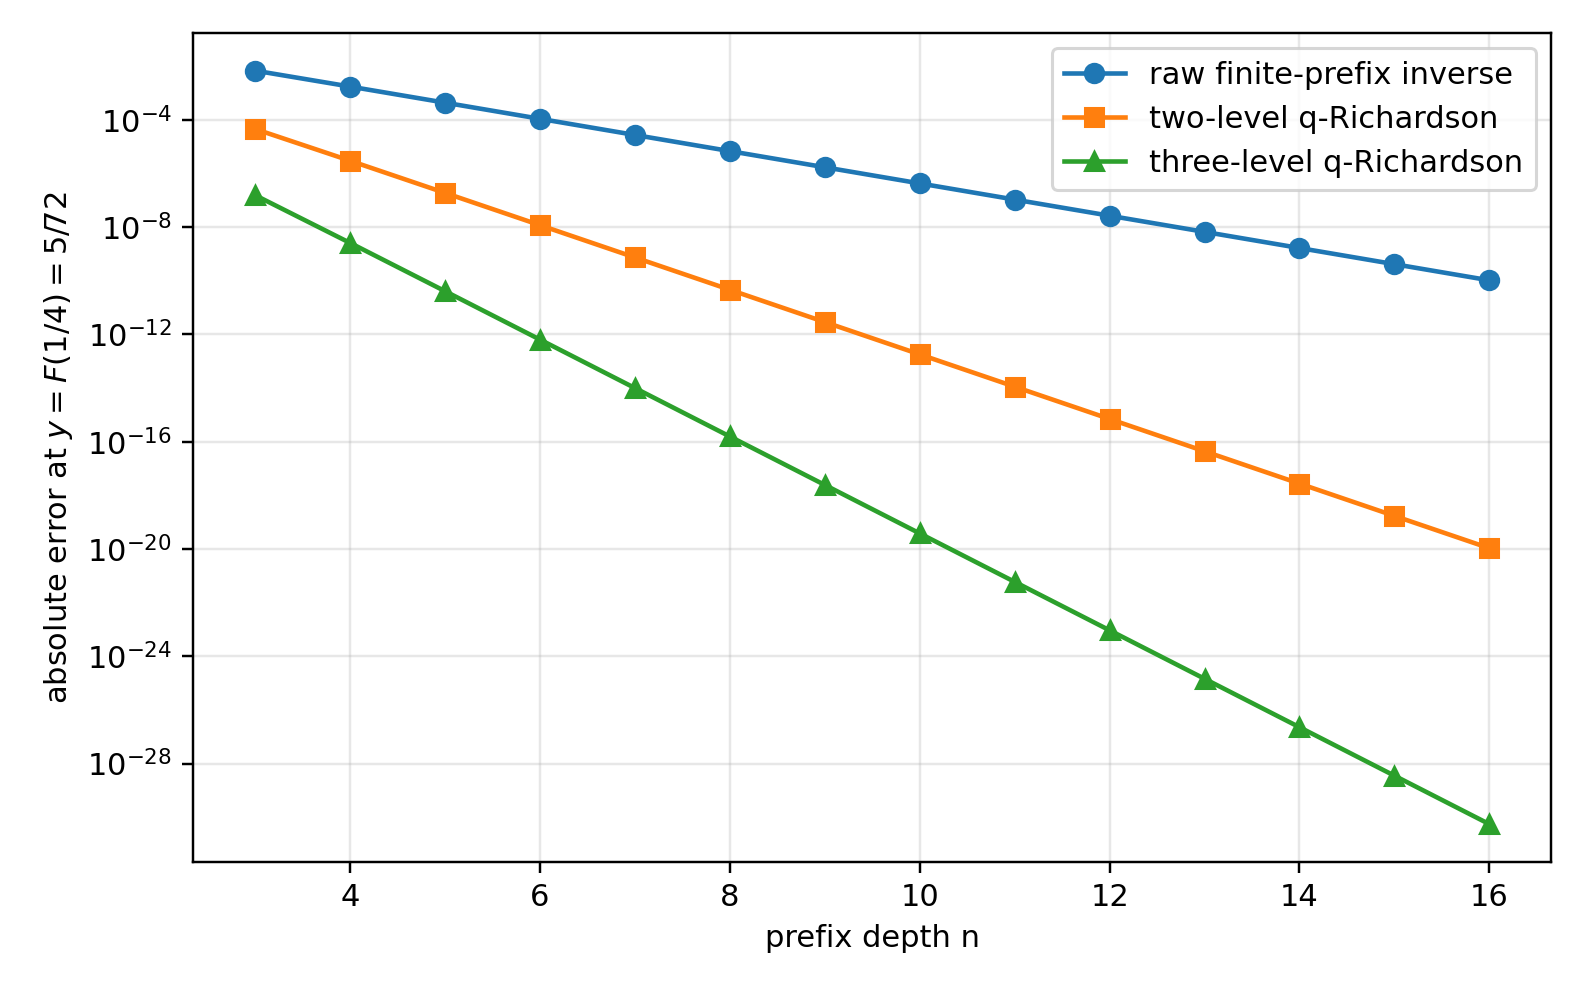
\includegraphics[width=0.92\textwidth]{assets/Fabius_Inverse_Frontier_Report_Source_and_PDF/figures/quarter_quantile_richardson.png}
\caption{Raw and accelerated errors at the exact output $F(1/4)=5/72$.  The
straight-line separation on the logarithmic scale reflects the exact geometric orders
$4^{-n}$, $16^{-n}$, and $64^{-n}$.}
\label{p1:fig:quarter-richardson}
\end{figure}

\subsection{Exact sign and two-sided bounds for every accelerated quarter error}

The preceding asymptotic constants can be strengthened to a finite-$n$ interpolation
statement.  Put
\begin{equation}
 f(Q):=\Delta_2(Q)=\frac{\sqrt{1+(64/9)Q}-1}{8}.
 \label{p1:eq:f-quarter-germ}
\end{equation}
For fixed $n$ and $s$, the quantity
$\mathcal G_{n,s}(5/72)-1/4$ is the value at $Q=0$ of the polynomial of degree
at most $s-1$ interpolating $f$ at the nodes
$4^{-n},4^{-(n+1)},\ldots,4^{-(n+s-1)}$.

\begin{theorem}[Positive accelerated errors and sharp finite-depth bounds]
\label{p1:thm:quarter-positive-bounds}
Let
\begin{equation}
 K_s:=\frac{C_{s-1}2^{-s^2+5s-2}}{9^s}.
 \label{p1:eq:Ks-quarter}
\end{equation}
For every $s\ge1$ and $n\ge3$,
\begin{equation}
 \boxed{
 0< K_s4^{-sn}\left(1+\frac{64}{9}4^{-n}\right)^{\frac12-s}
 <\mathcal G_{n,s}\!\left(\frac5{72}\right)-\frac14
 <K_s4^{-sn}.}
 \label{p1:eq:quarter-two-sided}
\end{equation}
In particular, the ratio of the exact error to its leading term is squeezed to one
inside an explicitly shrinking enclosure.
\end{theorem}

\begin{proof}
Let $p_{n,s-1}$ be the Lagrange interpolant just described.  The interpolation
remainder at zero gives a point $\xi_{n,s}\in(0,4^{-n})$ such that
\begin{equation}
 -p_{n,s-1}(0)
 =\frac{f^{(s)}(\xi_{n,s})}{s!}
   \prod_{j=0}^{s-1}(-4^{-(n+j)}).
 \label{p1:eq:Lagrange-remainder-quarter}
\end{equation}
Now
\begin{equation}
 f^{(s)}(Q)=\frac1{8}\left(\frac12\right)^{\!\underline{s}}
 \left(\frac{64}{9}\right)^s
 \left(1+\frac{64}{9}Q\right)^{\frac12-s},
 \label{p1:eq:f-quarter-derivative}
\end{equation}
where the falling factorial has sign $(-1)^{s-1}$.  The signs in
\eqref{p1:eq:Lagrange-remainder-quarter} therefore imply $p_{n,s-1}(0)>0$.
Using
\begin{equation}
 \frac{\left|\left(\frac12\right)^{\!\underline{s}}\right|}{8s!}
 \left(\frac{64}{9}\right)^s4^{-\binom s2}=K_s
 \label{p1:eq:Ks-identity}
\end{equation}
produces the middle expression in \eqref{p1:eq:quarter-two-sided} with
$\xi_{n,s}$ in place of either endpoint.  Since the exponent $1/2-s$ is
negative, evaluation at $0$ and $4^{-n}$ gives the two strict bounds.
\end{proof}

\begin{remark}
The positivity in \cref{p1:thm:quarter-positive-bounds} is not visible term-by-term in
\eqref{p1:eq:Catalan-qbinom-full}, whose tail alternates.  It is a consequence of the
complete monotonicity pattern of the derivatives of the square-root germ and the sign
of the Lagrange remainder.  This is one concrete place where exact interpolation gives
more information than formal Richardson cancellation.
\end{remark}

\begin{proposition}[Large-order Catalan coefficients]
\label{p1:prop:Catalan-large-order}
The Taylor coefficients of the quarter germ satisfy
\begin{equation}
 \boxed{
 \delta_{2,m}\sim
 (-1)^{m-1}\frac1{16\sqrt\pi}\left(\frac{64}{9}\right)^m m^{-3/2}.}
 \label{p1:eq:Catalan-large-order}
\end{equation}
Thus the branch point $Q=-9/64$ controls both the convergence radius and the
$m^{-3/2}$ algebraic prefactor.
\end{proposition}

\begin{proof}
Insert the classical Catalan asymptotic
$C_{m-1}\sim4^{m-1}/(\sqrt\pi\,m^{3/2})$ into
\eqref{p1:eq:Catalan-germ}.
\end{proof}

\subsection{A universal first coefficient at every inverse-dyadic anchor}

The leading displacement of the algebraic germ admits a particularly compact expression in
the dyadic moment numbers $d_r$ from \eqref{p1:eq:d-def}.

\begin{proposition}[First algebraic-germ coefficient]
\label{p1:prop:first-dyadic-germ-coefficient}
For every $r\ge2$,
\begin{equation}
 \boxed{
 \delta_{r,1}
 =\frac1{18}\frac{F''(2^{-r})}{F'(2^{-r})}
 =\frac{2^{r-1}(r-1)d_{r-2}}{9d_{r-1}}>0.}
 \label{p1:eq:first-dyadic-germ-coefficient}
\end{equation}
For $r=1$, $\Delta_1\equiv0$ and $G_n(1/2)=1/2$ exactly.
\end{proposition}

\begin{proof}
The first equality is \eqref{p1:eq:c1} evaluated at $x_r$.  Formula
\eqref{p1:eq:dyadic-jet} gives
\[
 \frac{F''(x_r)}{F'(x_r)}
 =4\frac{F(2^{2-r})}{F(2^{1-r})}.
\]
Substitute \eqref{p1:eq:d-def} at indices $r-2$ and $r-1$ and simplify the powers
of two.  Positivity follows from $d_j>0$.  The case $r=1$ follows from symmetry
of every prefix density.
\end{proof}

The values $4/9$, $8/5$, and $40/9$ in
\eqref{p1:eq:Catalan-first}, \eqref{p1:eq:Delta3}, and \eqref{p1:eq:Delta4} are therefore
not isolated coincidences; they are the first members of a single exact rational
sequence controlled by adjacent dyadic moments.

\section{Periodic Lambert--Bell inversion at the endpoint}
\label{p1:sec:endpoint-inversion}

\subsection{The forward input and its periodic data}

We now invert the all-orders small-$x$ expansion already established in the corpus.
Put
\begin{equation}
 L:=\log2,
 \qquad B:=1+\frac L2,
 \qquad \beta:=\frac BL=\frac1L+\frac12.
 \label{p1:eq:L-B-beta}
\end{equation}
For sufficiently small $x>0$, the exact lower-Lambert phase is the large positive
solution
\begin{equation}
 x=\lambda2^{-\lambda}=\lambda\e^{-L\lambda},
 \qquad
 \lambda(x)=-\frac1L W_{-1}(-Lx) \cite{p1:CorlessLambertW}.
 \label{p1:eq:exact-lower-Lambert}
\end{equation}
The sharp forward expansion has, for every fixed $N$, the form
\begin{equation}
 \boxed{
 \log F(x)=
 -\frac L2\lambda^2+B\lambda-\frac12\log\lambda
 +C_{\sharp}+\Psi(\lambda)
 +\sum_{j=1}^{N-1}\frac{A_j(\lambda)}{\lambda^j}
 +\bigO_N(\lambda^{-N}).}
 \label{p1:eq:forward-endpoint-all-orders}
\end{equation}
Here every $A_j$ and $\Psi$ is smooth, bounded, and one-periodic.  With
$\gamma$ denoting Euler's constant and $\gamma_1$ the first Stieltjes constant in the
convention
\(
 \zeta(s)=\frac1{s-1}+\sum_{m\ge0}(-1)^m\gamma_m(s-1)^m/m!
\),
\begin{equation}
 C_{\sharp}=
 \frac{6\gamma^2+12\gamma_1-\pi^2}{12L}
 -\frac{7L}{12}-\frac12\log\pi.
 \label{p1:eq:Csharp}
\end{equation}
The zero-mean periodic fluctuation has Fourier coefficients
\begin{equation}
 \Psi(u)=\sum_{k\ne0}\widehat\Psi(k)\e^{2\pi\ii ku},
 \qquad
 \widehat\Psi(k)=-\frac{\Gamma(-\chi_k)\zeta(1-\chi_k)}{L},
 \qquad
 \chi_k=\frac{2\pi\ii k}{L}.
 \label{p1:eq:Psi-Fourier}
\end{equation}
The first logarithmic correction is
\begin{equation}
 \boxed{
 A_1(u)=\frac1{24}+\frac1{2L}
 -\frac{\Psi''(u)+\Psi'(u)^2}{2L^2}.}
 \label{p1:eq:A1-periodic}
\end{equation}
The Gamma factor in \eqref{p1:eq:Psi-Fourier} gives exponential Fourier decay, so all
phase differentiations below are legitimate.

\subsection{Two-scale inversion of the saddle phase}

Let
\begin{equation}
 T:=\log\frac1y,
 \qquad
 \rho:=\sqrt{\frac{2T}{L}},
 \qquad
 \theta:=\rho+\beta.
 \label{p1:eq:T-rho-theta}
\end{equation}
The leading inverse equivalent from the corpus is conveniently written
\begin{equation}
 G_0(y):=\rho\e^{-L\rho-L\beta}
 =\frac{\sqrt T}{\e\sqrt L}\e^{-\sqrt{2LT}}.
 \label{p1:eq:G0}
\end{equation}
The following theorem computes what the corpus left implicit.

\begin{theorem}[Phase inversion through two nontrivial orders]
\label{p1:thm:phase-two-orders}
As $y\downarrow0$, the exact phase of $x=G(y)$ satisfies
\begin{equation}
 \boxed{
 \lambda(G(y))=
 \rho+\beta+\frac{d_1}{\rho}+\frac{d_2}{\rho^2}
 +\bigO\!\left(\frac{(\log\rho)^2}{\rho^3}\right),}
 \label{p1:eq:lambda-inverse-two-orders}
\end{equation}
where all periodic functions below are evaluated at $\theta$ and
\begin{align}
 d_1&=\frac{\beta^2}{2}
 +\frac{C_{\sharp}+\Psi(\theta)-\tfrac12\log\rho}{L},
 \label{p1:eq:d1-endpoint}\\
 d_2&=\frac{\Psi'(\theta)d_1+A_1(\theta)-\tfrac12\beta}{L}.
 \label{p1:eq:d2-endpoint}
\end{align}
Consequently,
\begin{equation}
 \boxed{
 \log\frac{G(y)}{G_0(y)}
 =\frac{h_1}{\rho}+\frac{h_2}{\rho^2}
 +\bigO\!\left(\frac{(\log\rho)^3}{\rho^3}\right),}
 \label{p1:eq:log-inverse-two-orders}
\end{equation}
with
\begin{align}
 h_1&=\beta-Ld_1
 =\frac12\log\rho+\kappa_0-\Psi(\theta),
 \label{p1:eq:h1}\\
 h_2&=d_1-\frac{\beta^2}{2}-Ld_2
 =(1-\Psi'(\theta))d_1-\frac{\beta^2}{2}
   -A_1(\theta)+\frac\beta2,
 \label{p1:eq:h2}\\
 \kappa_0&:=\beta-\frac L2\beta^2-C_{\sharp}
 =\frac1{2L}-\frac L8-C_{\sharp}.
 \label{p1:eq:kappa0}
\end{align}
Equivalently, in multiplicative form,
\begin{equation}
 \boxed{
 \frac{G(y)}{G_0(y)}
 =1+\frac{h_1}{\rho}
 +\frac{h_2+\tfrac12h_1^2}{\rho^2}
 +\bigO\!\left(\frac{(\log\rho)^3}{\rho^3}\right).}
 \label{p1:eq:inverse-multiplicative-two-orders}
\end{equation}
\end{theorem}

\begin{proof}
Negate \eqref{p1:eq:forward-endpoint-all-orders} and use
$T=L\rho^2/2$.  Write
\begin{equation}
 \lambda=\rho+\beta+D,
 \qquad
 D=\frac{d_1}{\rho}+\frac{d_2}{\rho^2}+\cdots.
 \label{p1:eq:lambda-D}
\end{equation}
The quadratic part simplifies exactly:
\begin{equation}
 \frac L2\lambda^2-B\lambda
 =\frac L2\rho^2+L\rho D-\frac L2\beta^2+\frac L2D^2.
 \label{p1:eq:quadratic-cancellation}
\end{equation}
The constant term after cancellation of $L\rho^2/2$ is
\[
 Ld_1-\frac L2\beta^2+\frac12\log\rho-C_{\sharp}-\Psi(\theta),
\]
which gives \eqref{p1:eq:d1-endpoint}.  The coefficient of $\rho^{-1}$ is
\[
 Ld_2+\frac\beta2-\Psi'(\theta)d_1-A_1(\theta),
\]
which gives \eqref{p1:eq:d2-endpoint}.  The all-orders remainder in
\eqref{p1:eq:forward-endpoint-all-orders}, together with $d_1=\bigO(\log\rho)$,
then yields the stated phase remainder by one Newton correction; the derivative of the
phase equation is $L\rho+\bigO(1)$.

Finally,
\begin{align*}
 \log G(y)
 &=\log\lambda-L\lambda\\
 &=\log\rho-L\rho-L\beta
   +\log\!\left(1+\frac\beta\rho+\frac D\rho\right)-LD.
\end{align*}
Expansion through $\rho^{-2}$ gives \eqref{p1:eq:h1}--\eqref{p1:eq:h2}; exponentiation
gives \eqref{p1:eq:inverse-multiplicative-two-orders}.
\end{proof}

The first consequence is the promised explicit correction to the leading equivalent.

\begin{corollary}[First oscillatory relative correction]
\label{p1:cor:first-oscillatory-inverse}
As $y\downarrow0$,
\begin{equation}
 \boxed{
 \frac{G(y)}{G_0(y)}
 =1+\frac{\tfrac12\log\rho+\kappa_0-\Psi(\rho+\beta)}{\rho}
 +\bigO\!\left(\frac{(\log\rho)^2}{\rho^2}\right).}
 \label{p1:eq:first-oscillatory-inverse}
\end{equation}
\end{corollary}

\begin{remark}[Why the exact phase shift matters]
Replacing $\rho+\beta$ by $\rho$, or replacing $\rho$ by a cruder expression in
$\log(1/y)$ inside $\Psi$, changes the phase by a fixed noninteger amount and therefore
changes the correction at its full natural size $1/\rho$.  The constant shift
$\beta=1/L+1/2$ is not optional bookkeeping.
\end{remark}

\subsection{A complete periodic limit set}

The oscillation in \eqref{p1:eq:first-oscillatory-inverse} cannot be absorbed into a
constant second term.

\begin{theorem}[Limit set of the normalized second term]
\label{p1:thm:inverse-limit-set}
Define
\begin{equation}
 \mathscr R(y):=
 \rho\left(\frac{G(y)}{G_0(y)}-1\right)-\frac12\log\rho.
 \label{p1:eq:R-limit-set}
\end{equation}
Then the complete set of subsequential limits as $y\downarrow0$ is
\begin{equation}
 \boxed{
 \range_{y\downarrow0}\mathscr R(y)
 =\bigl[\kappa_0-\max_{u\in[0,1]}\Psi(u),
         \ \kappa_0-\min_{u\in[0,1]}\Psi(u)\bigr].}
 \label{p1:eq:inverse-limit-interval}
\end{equation}
The interval is nondegenerate.  Hence there is no constant $c$ for which
\begin{equation}
 \frac{G(y)}{G_0(y)}
 =1+\frac{\tfrac12\log\rho+c}{\rho}+\smallo(\rho^{-1}).
 \label{p1:eq:no-constant-second-term}
\end{equation}
\end{theorem}

\begin{proof}
Corollary \ref{p1:cor:first-oscillatory-inverse} gives
\begin{equation}
 \mathscr R(y)=\kappa_0-\Psi(\rho+\beta)
 +\bigO\!\left(\frac{(\log\rho)^2}{\rho}\right).
 \label{p1:eq:R-phase}
\end{equation}
As $y$ ranges down to zero, $\rho$ ranges continuously to $+\infty$.  For any
$u\in[0,1)$, choose $\rho_m=m+u-\beta$ and
$y_m=\exp(-L\rho_m^2/2)$.  Then the phase in \eqref{p1:eq:R-phase} is exactly
$u$ modulo one, proving that every value of $\kappa_0-\Psi$ is a subsequential
limit.  Conversely, compactness of the phase circle shows that every sequence has a
phase-convergent subsequence, so no other limit can occur.

The Fourier coefficient $\widehat\Psi(1)$ in \eqref{p1:eq:Psi-Fourier} is nonzero:
Gamma has no zeros and the classical zero-free line $\Re s=1$ gives
$\zeta(1-\chi_1)\ne0$ \cite{p1:TitchmarshZeta}.  Thus $\Psi$ is nonconstant and the interval has positive
length.  Formula \eqref{p1:eq:no-constant-second-term} would force a singleton limit set,
a contradiction.
\end{proof}

\subsection{Quantile elasticity and inverse derivatives}

The logarithmic derivative of the inverse is often more stable numerically than $G'$ itself.

\begin{theorem}[Two-term endpoint elasticity]
\label{p1:thm:quantile-elasticity}
As $y\downarrow0$,
\begin{equation}
 \boxed{
 \frac{yG'(y)}{G(y)}
 =\frac1\rho+\frac{\Psi'(\rho+\beta)-1}{L\rho^2}
 +\bigO\!\left(\frac{\log\rho}{\rho^3}\right).}
 \label{p1:eq:quantile-elasticity}
\end{equation}
Consequently,
\begin{equation}
 G'(y)=\frac{G(y)}{y\rho}
 \left[1+\frac{\Psi'(\rho+\beta)-1}{L\rho}
 +\bigO\!\left(\frac{\log\rho}{\rho^2}\right)\right].
 \label{p1:eq:Gprime-endpoint}
\end{equation}
\end{theorem}

\begin{proof}
Regard both $T=-\log y$ and $\log x$ as functions of the exact phase $\lambda$.
Differentiating \eqref{p1:eq:forward-endpoint-all-orders} gives
\begin{equation}
 \frac{yG'(y)}{G(y)}
 =-\frac{\dd\log x/\dd\lambda}{\dd T/\dd\lambda}
 =\frac{L-\lambda^{-1}}
 {L\lambda-B+\tfrac1{2\lambda}-\Psi'(\lambda)+\bigO(\lambda^{-2})}.
 \label{p1:eq:elasticity-exact-ratio}
\end{equation}
Insert $\lambda=\rho+\beta+\bigO((\log\rho)/\rho)$ and expand.  The terms
containing $\beta$ cancel from the denominator because $B=L\beta$, leaving
\eqref{p1:eq:quantile-elasticity}.
\end{proof}

By reflection, every formula in this section has a right-endpoint counterpart: replace
$y$ by $1-y$ and $G(y)$ by $1-G(y)$.  In particular, the same periodic function and
the same phase shift govern the two ends.

\subsection{An all-orders Lambert--Bell reversion algorithm}

The preceding calculation extends mechanically to every order, but ordinary power-series
notation hides the two-scale nature of the coefficients.  Treat $z=1/\rho$ as the small
variable while holding the fast phase $\theta=\rho+\beta$ and the slow logarithm
$\log\rho$ as coefficient variables.  Let
\begin{equation}
 D(z)=\sum_{m\ge1}d_mz^m,
 \qquad
 \lambda=\rho+\beta+D(z).
 \label{p1:eq:D-formal}
\end{equation}
Define
\begin{align}
 \mathcal R(z,D):={}&-\frac L2\beta^2+\frac L2D^2+\frac12\log\rho
 +\frac12\log(1+\beta z+zD)-C_{\sharp}-\Psi(\theta+D)
 \notag\\
 &-\sum_{j\ge1}A_j(\theta+D)z^j(1+\beta z+zD)^{-j}.
 \label{p1:eq:R-formal-endpoint}
\end{align}
The phase equation is formally
\begin{equation}
 0=\frac LzD+\mathcal R(z,D).
 \label{p1:eq:phase-formal-equation}
\end{equation}

\begin{theorem}[Triangular all-orders endpoint recursion]
\label{p1:thm:all-orders-endpoint-recursion}
Let $D_m(z)=\sum_{j=1}^{m}d_jz^j$ and set $D_0=0$.  The unique formal
solution of \eqref{p1:eq:phase-formal-equation} is generated by
\begin{equation}
 \boxed{
 d_{m+1}=-\frac1L[z^m]\mathcal R(z,D_m),
 \qquad m\ge0.}
 \label{p1:eq:d-all-orders-recursion}
\end{equation}
Each $d_m$ is a polynomial in $\log\rho$ with coefficients in the differential algebra
generated by the periodic functions $\Psi,A_1,\ldots,A_{m-1}$.

Write
\begin{equation}
 \log\frac{G(y)}{G_0(y)}
 =\log(1+\beta z+zD)-LD
 =\sum_{m\ge1}h_mz^m.
 \label{p1:eq:h-all-orders}
\end{equation}
Then the multiplicative coefficients $g_m$ in
\begin{equation}
 \frac{G(y)}{G_0(y)}\sim1+\sum_{m\ge1}g_m\rho^{-m}
 \label{p1:eq:g-all-orders}
\end{equation}
are the complete Bell polynomials
\begin{equation}
 \boxed{
 g_m=\frac1{m!}\mathcal B_m(1!h_1,2!h_2,\ldots,m!h_m).}
 \label{p1:eq:g-Bell}
\end{equation}
For every fixed truncation order, the resulting expansion is rigorous with a remainder
uniform in the phase.
\end{theorem}

\begin{proof}
The coefficient of $d_{m+1}$ in $[z^m](L D/z)$ is exactly $L$, while
$[z^m]\mathcal R$ depends only on $d_1,\ldots,d_m$.  This gives the triangular
recursion.  Taylor expansion of each periodic coefficient at $\theta$ shows inductively
that the coefficient algebra is closed under the required operations.  Formula
\eqref{p1:eq:g-Bell} is the standard exponential formula applied to
\eqref{p1:eq:h-all-orders}.  The uniform all-orders remainder in
\eqref{p1:eq:forward-endpoint-all-orders}, together with the fact that the derivative of the
phase equation is asymptotic to $L\rho$, upgrades the formal induction to a Poincare
expansion at any fixed order.
\end{proof}

\begin{boxedremark}
The endpoint inverse has a mixed asymptotic architecture:
\[
 \text{lower Lambert }W
 \quad+\quad \text{polynomials in }\log\rho
 \quad+\quad \text{periodic Gamma--zeta jets}
 \quad+\quad \text{Bell reversion}.
\]
None of these four layers can be removed without losing a term at some finite order.
\end{boxedremark}

\section{Symbolic, exact, and high-precision verification}
\label{p1:sec:verification}

\subsection{Exact rational checks of the local-polynomial theorem}

The construction of $\mathcal A_r$ was checked independently in exact rational
arithmetic by the following pipeline:
\begin{enumerate}
 \item generate $d_0,\ldots,d_r$ from the recurrence
 \begin{equation}
 d_m=\frac{\sum_{k=0}^{m-1}\binom{m+1}{k}d_k}
 {(m+1)(2^m-1)};
 \label{p1:eq:d-recurrence-check}
 \end{equation}
 \item form the dyadic jet $J_r$ from \eqref{p1:eq:Jr};
 \item generate $b_j$ from \eqref{p1:eq:b-rec};
 \item apply the finite operator in \eqref{p1:eq:Ar-def};
 \item substitute the resulting root series into $\mathcal A_r$ and verify vanishing
 coefficient-by-coefficient.
\end{enumerate}
For $r\le12$, all coefficients through $Q^{12}$ vanish exactly after substitution.
For $r=2$, direct substitution of the radical in \eqref{p1:eq:quarter-exact} reduces the
identity to zero without series expansion.

\subsection{Quarter-anchor convergence and exact enclosures}

\begin{table}[ht]
\centering
\small
\begin{tabular}{@{}r rr rr rr@{}}
\toprule
$n$ & raw error & ratio & $s=2$ error & ratio & $s=3$ error & ratio \\
\midrule
3 & $6.76157\,10^{-3}$ & 0.973666 & $4.51028\,10^{-5}$ & 0.935251 & $1.53350\,10^{-7}$ & 0.915801 \\
4 & $1.72422\,10^{-3}$ & 0.993150 & $2.96269\,10^{-6}$ & 0.982949 & $2.55798\,10^{-9}$ & 0.977675 \\
5 & $4.33277\,10^{-4}$ & 0.998270 & $1.87566\,10^{-7}$ & 0.995679 & $4.06494\,10^{-11}$ & 0.994333 \\
6 & $1.08460\,10^{-4}$ & 0.999566 & $1.17610\,10^{-8}$ & 0.998916 & $6.37859\,10^{-13}$ & 0.998578 \\
7 & $2.71238\,10^{-5}$ & 0.999892 & $7.35660\,10^{-10}$ & 0.999729 & $9.97719\,10^{-15}$ & 0.999644 \\
8 & $6.78150\,10^{-6}$ & 0.999973 & $4.59881\,10^{-11}$ & 0.999932 & $1.55935\,10^{-16}$ & 0.999911 \\
\bottomrule
\end{tabular}
\caption{Exact quarter-quantile errors.  Each ratio divides by the corresponding
leading term in \eqref{p1:eq:quarter-raw-law}--\eqref{p1:eq:quarter-R3-law}.  The values
lie inside the analytic enclosure \eqref{p1:eq:quarter-two-sided}.}
\label{p1:tab:quarter-errors}
\end{table}

The table illustrates a useful distinction.  Richardson acceleration does not merely make
the error small: the exact square-root germ supplies a certified sign and a certified
finite-$n$ relative enclosure.  At $n=8$, three levels already reduce the absolute error
below $1.6\times10^{-16}$.

\subsection{Endpoint inversion on exact dyadic test values}

For $y_n=F(2^{-n})$, the true inverse is exactly $G(y_n)=2^{-n}$.  The dyadic moment
recurrence therefore provides endpoint test values without numerical root finding.  Define
\begin{align}
 G^{[0]}(y)&:=G_0(y),\label{p1:eq:Gapprox0}\\
 G^{[1]}(y)&:=G_0(y)\exp(h_1/\rho),\label{p1:eq:Gapprox1}\\
 G^{[2]}(y)&:=G_0(y)\exp(h_1/\rho+h_2/\rho^2).
 \label{p1:eq:Gapprox2}
\end{align}
The periodic function and its first two derivatives were evaluated from
\eqref{p1:eq:Psi-Fourier} with nine positive Fourier modes at 100 decimal digits.

\begin{table}[ht]
\centering
\small
\begin{tabular}{@{}r r r r r@{}}
\toprule
$n$ & $\rho$ & relative error of $G^{[0]}$ & of $G^{[1]}$ & of $G^{[2]}$ \\
\midrule
5   & 6.43984  & $-3.82510\,10^{-1}$ & $ 7.89489\,10^{-2}$ & $-2.16957\,10^{-2}$ \\
10  & 12.08040 & $-2.56964\,10^{-1}$ & $ 2.68825\,10^{-2}$ & $-4.39948\,10^{-3}$ \\
20  & 22.82438 & $-1.61765\,10^{-1}$ & $ 8.76101\,10^{-3}$ & $-8.23920\,10^{-4}$ \\
40  & 43.65176 & $-9.65552\,10^{-2}$ & $ 2.71602\,10^{-3}$ & $-1.43280\,10^{-4}$ \\
80  & 84.54102 & $-5.53439\,10^{-2}$ & $ 8.04968\,10^{-4}$ & $-2.34032\,10^{-5}$ \\
100 &104.83719 & $-4.59578\,10^{-2}$ & $ 5.39809\,10^{-4}$ & $-1.29189\,10^{-5}$ \\
\bottomrule
\end{tabular}
\caption{Relative errors at the exact points $y_n=F(2^{-n})$.  The first and
second inverse corrections successively remove the dominant endpoint error.}
\label{p1:tab:endpoint-errors}
\end{table}

\begin{figure}[ht]
\centering
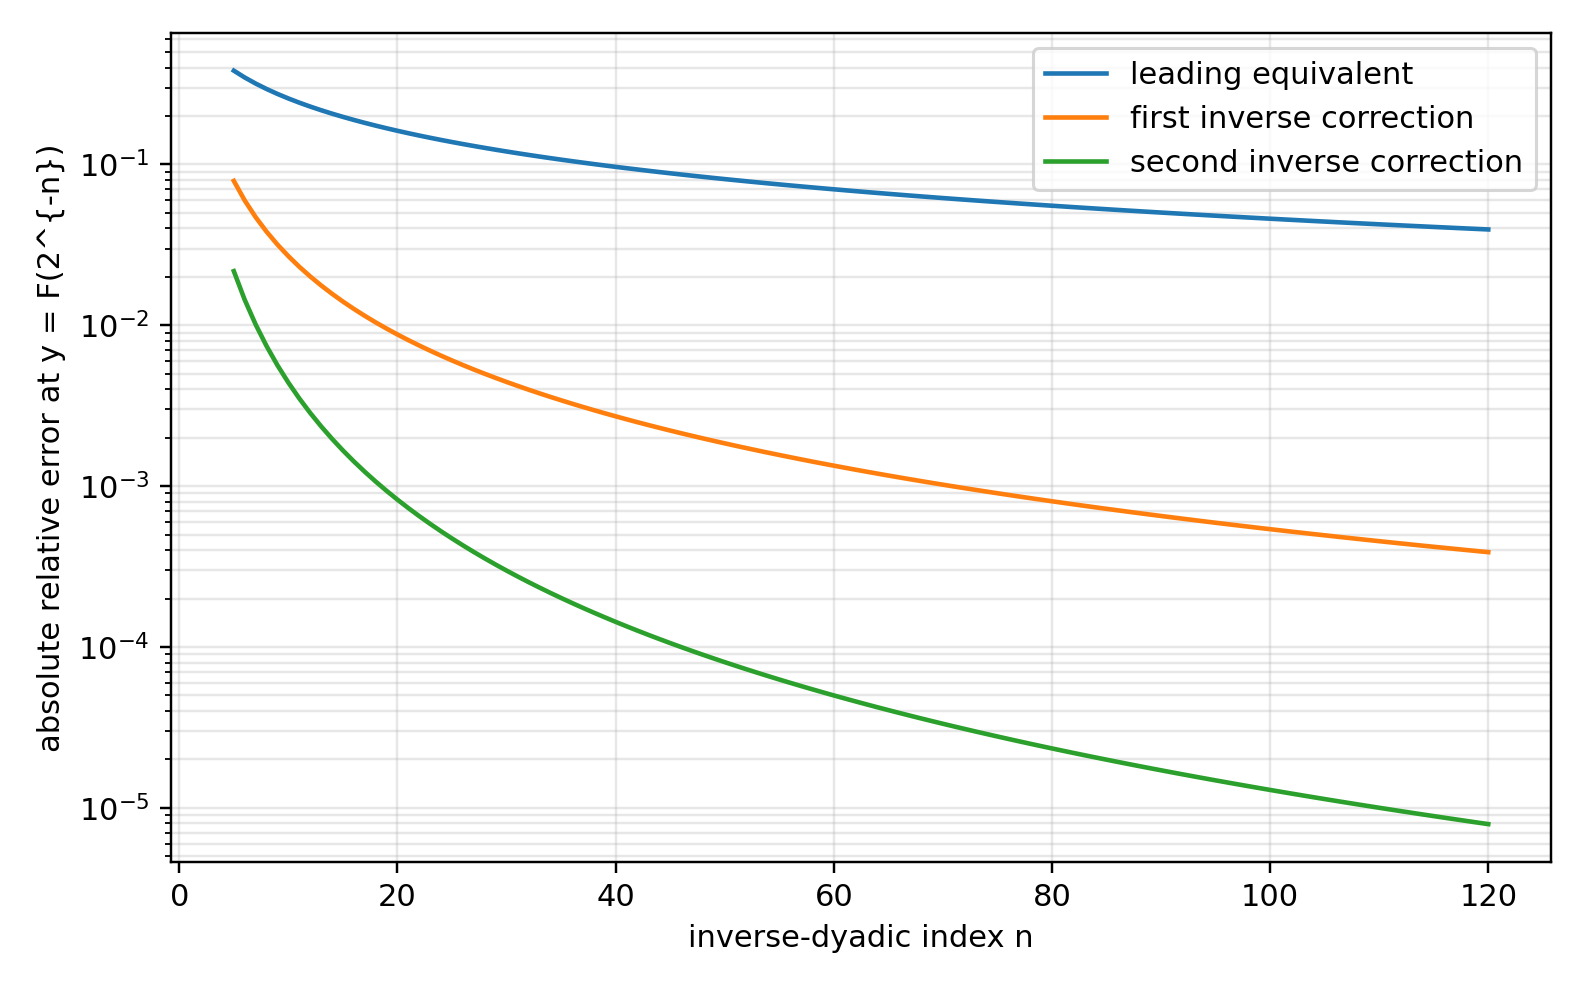
\includegraphics[width=0.92\textwidth]{assets/Fabius_Inverse_Frontier_Report_Source_and_PDF/figures/endpoint_inverse_errors.png}
\caption{Absolute relative errors of the leading, first-corrected, and second-corrected
endpoint inverse approximations on exact inverse-dyadic test values.}
\label{p1:fig:endpoint-errors}
\end{figure}

Numerically,
\begin{equation}
 \begin{split}
 L&=0.6931471805599453094\ldots,\\
 \beta&=1.9426950408889634074\ldots,\\
 C_{\sharp}&=-2.0279838986388594240\ldots,\\
 \kappa_0&=2.6626880215133479640\ldots.
 \end{split}
 \label{p1:eq:endpoint-constants-numeric}
\end{equation}
The first Fourier coefficient has
\begin{equation}
 |\widehat\Psi(1)|=1.0627109779221651\times10^{-6},
 \qquad
 \arg\widehat\Psi(1)=-0.7795055208985225\ldots,
 \label{p1:eq:first-Psi-mode}
\end{equation}
and the second mode is smaller by a factor about $6.30\times10^{-7}$.  Thus $\Psi$ is
very close to a single sinusoid, although its small amplitude does not make it
asymptotically dispensable.

\begin{figure}[ht]
\centering
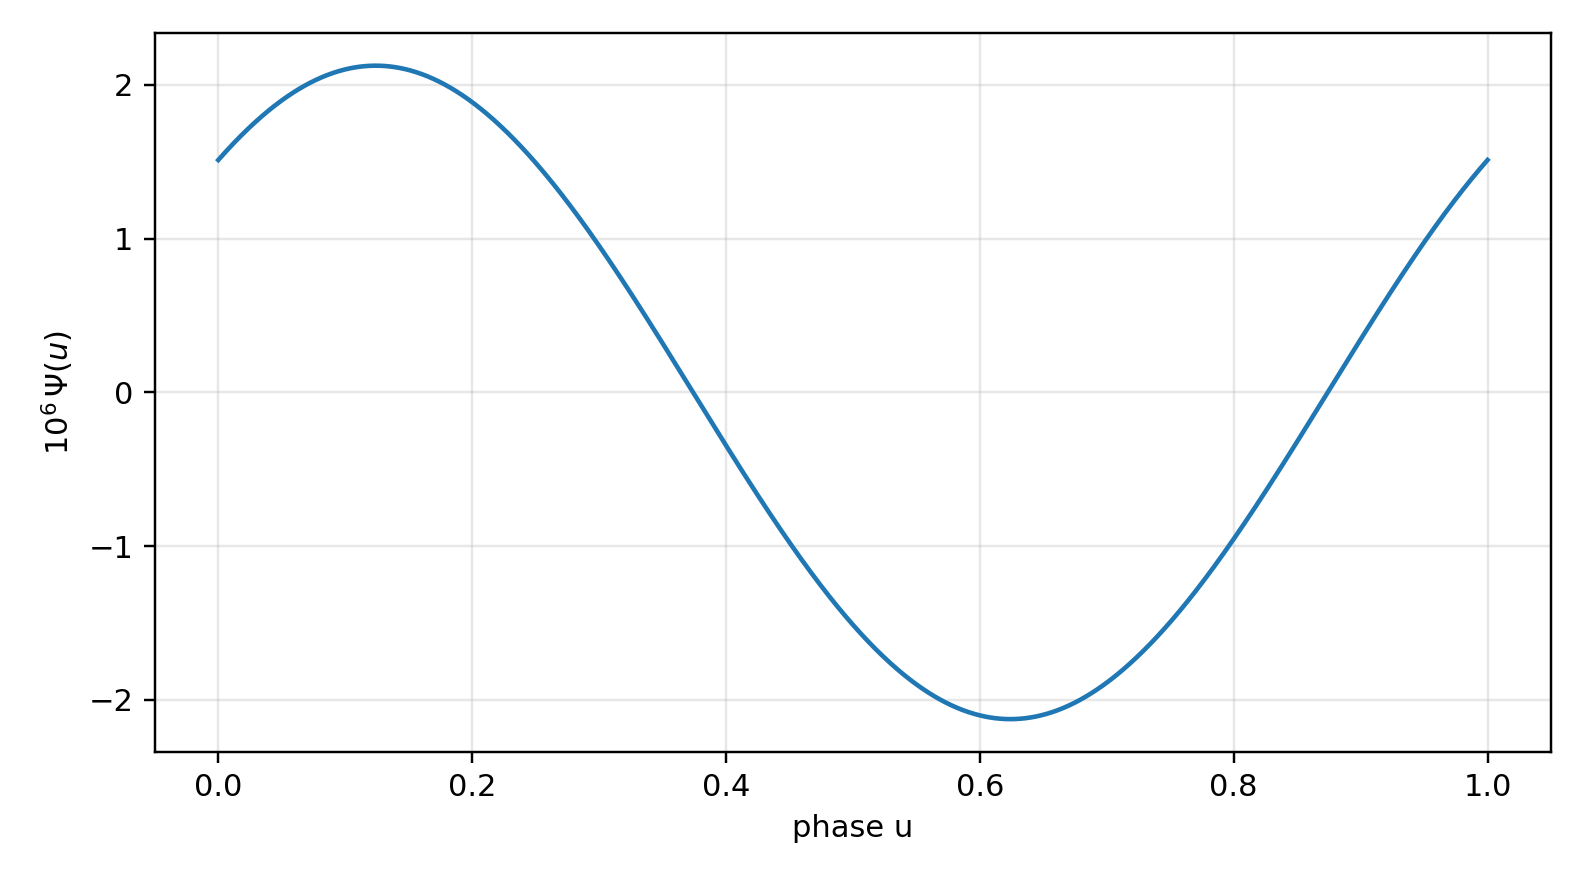
\includegraphics[width=0.92\textwidth]{assets/Fabius_Inverse_Frontier_Report_Source_and_PDF/figures/periodic_inverse_phase.png}
\caption{The periodic Gamma--zeta fluctuation.  The vertical scale is multiplied by
$10^6$.  A grid evaluation gives approximately
$\min\Psi=-2.1254264\times10^{-6}$ and
$\max\Psi=2.1254241\times10^{-6}$.}
\label{p1:fig:Psi-phase}
\end{figure}

The numerical range in \cref{p1:fig:Psi-phase} turns the abstract interval
\eqref{p1:eq:inverse-limit-interval} into an interval of width approximately
$4.25085\times10^{-6}$ centered extremely close to $\kappa_0$.  The width is tiny,
but it is fixed; multiplying the relative error by $\rho$ reveals it rather than erasing it.

\subsection{Independent checks and failure modes}

Three independent representations were used wherever possible:
\begin{enumerate}
 \item exact rational recurrences for $d_r$, $y_r$, $J_r$, and the coefficients of
 $\mathcal A_r$;
 \item symbolic series reversion, including direct residual checks
 $\mathcal A_r(\Delta_r(Q),Q)=\bigO(Q^{M+1})$;
 \item high-precision evaluation of the Gamma--zeta Fourier series and exact dyadic
 inverse test points.
\end{enumerate}
The principal numerical failure mode is phase corruption: replacing the exact
$\theta=\rho+\beta$ by a rounded or asymptotically simplified phase can dominate the
very small periodic signal.  The principal algebraic failure mode is confusing the
forward coefficient $-b_1F''$ with the inverse coefficient $b_1F''/F'$; the missing
Jacobian changes every Richardson constant.

\section{Algorithms and a Lean formalization roadmap}
\label{p1:sec:algorithms-formalization}

\subsection{Exact construction of an inverse-dyadic germ}

The following pseudocode is entirely rational up to the final algebraic root or formal
series operation.

\begin{lstlisting}[style=pseudo,caption={Exact construction of the local polynomial and inverse germ.},label={lst:dyadic-germ}]
input: anchor depth r, requested series order M

# Dyadic moment numbers
D[0] = 1
for m = 1..r:
    D[m] = sum(binomial(m+1,k)*D[k], k=0..m-1)
           / ((m+1)*(2^m-1))

# Reciprocal-sinc coefficients
b[0] = 1
for j = 1..floor(r/2):
    gamma[j] = zeta(2*j)/(j*pi^(2*j)*(4^j-1))  # rational after simplification
    b[j] = sum(k*gamma[k]*b[j-k], k=1..j)/j

# Terminating Fabius jet
J(z) = sum(
    2^(binomial(k+1,2)-binomial(r-k,2))
    * D[r-k] * z^k / (k!*(r-k)!),
    k=1..r)

# Exact finite-prefix local polynomial
A(z,Q) = J(z)
for j = 1..floor(r/2):
    A(z,Q) += (-1)^j * b[j] * Q^j * derivative(J,z,2*j)

# Formal inverse branch A(Delta(Q),Q)=0
Delta(Q) = 0
for m = 1..M:
    residual = coefficient(A(Delta(Q),Q), Q, m)
    delta[m] = -residual / derivative(J,z,1).subs(z=0)
    Delta(Q) += delta[m]*Q^m

return A(z,Q), Delta(Q)
\end{lstlisting}

For $r=2$, a radical solver should be used instead of formal reversion.  For larger $r$,
formal reversion is usually preferable to radicals: it preserves rationality, scales to high
order, and feeds directly into the Gaussian-binomial residual formula.

\subsection{Endpoint coefficient engine}

The all-orders endpoint recursion can be implemented in a differential polynomial ring whose
atoms are $\log\rho$, $\Psi^{(k)}(\theta)$, and $A_j^{(k)}(\theta)$.

\begin{lstlisting}[style=pseudo,caption={Lambert--Bell inverse coefficient engine.},label={lst:endpoint-engine}]
input: desired inverse order N; forward periodic coefficients A[1..N-1]
z = formal variable
D = 0
for m = 0..N-1:
    R = -L*beta^2/2 + L*D^2/2 + log(rho)/2
        + log(1 + beta*z + z*D)/2 - Csharp
        - Taylor_phase(Psi, theta, D)
        - sum(
            Taylor_phase(A[j],theta,D)
            * z^j * (1+beta*z+z*D)^(-j),
            j=1..N-1)
    d[m+1] = -coefficient(R,z,m)/L
    D += d[m+1]*z^(m+1)

H = truncate(log(1+beta*z+z*D)-L*D, z, N)
for m = 1..N:
    h[m] = coefficient(H,z,m)
    g[m] = CompleteBell(m, 1!*h[1], ..., m!*h[m]) / m!
return d, h, g
\end{lstlisting}

The supplied reproducibility script evaluates the first two orders directly rather than
building a general symbolic differential ring, but its formulas are exact transcriptions of
\cref{p1:thm:phase-two-orders}.

\subsection{Formalization modules}

The results separate naturally into five Lean-sized packages.

\begin{obligation}[Polynomial smoothing and inverse moment operator]
Formalize that, for a polynomial $q$ of degree at most $r$,
\[
 M(aD)q=J \quad\Longrightarrow\quad
 q=\sum_{j=0}^{\lfloor r/2\rfloor}(-1)^jb_ja^{2j}D^{2j}J.
\]
This requires only finite sums after the degree bound is known; no convergence theorem for
formal differential operators is needed.
\end{obligation}

\begin{obligation}[Plateau-to-polynomial localization]
Connect the existing almost-everywhere derivative plateau for $p_n^{(r)}$ to the statement
that $p_n$ agrees with a degree-$r$ polynomial on the closed interval
$[\xi_r-2^{-n},\xi_r+2^{-n}]$.  The clean route is repeated absolute continuity of the
spline pieces.
\end{obligation}

\begin{obligation}[Algebraic inverse germ]
Instantiate a formal implicit-function theorem over $\Q[[Q]]$ for
$\mathcal A_r(z,Q)$ with invertible linear coefficient $F'(x_r)$.  Prove separately that
the formal series is represented by the analytic local inverse and enters the plateau interval
for all large $n$.
\end{obligation}

\begin{remark}[Formalized geometric Lagrange core]
The former obligation to formalize \eqref{p1:eq:all-filter-moments} is discharged
at post-snapshot checkpoint
\nolinkurl{1e761ed77583e9870ceeaeb2c74ac824094f0f3f}.  The reusable layer in
\path{CompleteHomogeneous.lean} consists of
\nolinkurl{completeHomogeneousEval_smul},
\nolinkurl{completeHomogeneousEval_option_zero},
\nolinkurl{completeHomogeneousEval_fin_succ},
\nolinkurl{completeHomogeneousEvalOn_range}, and
\nolinkurl{completeHomogeneousEvalAt_zero}.  Over every commutative semiring,
\path{GeometricCompleteHomogeneous.lean} gives
\[
 h_n(1,q,\ldots,q^p)=\qbinom{n+p}{p}{q},
 \qquad
 h_n(c,cq,\ldots,cq^p)=c^n\qbinom{n+p}{p}{q}
\]
through \nolinkurl{completeHomogeneousEval_geometric},
\nolinkurl{completeHomogeneousEval_scaled_geometric}, and the range bridge
\nolinkurl{completeHomogeneousEvalOn_range_pow_eq_gaussianBinomial}.

Over every commutative ring,
\nolinkurl{sum_weight_mul_scaled_geometric_pow_succ_add} and
\nolinkurl{sum_weight_mul_scaled_geometric_pow_of_pos} assume exactness
directly on the nodes \(c q^j\); no nonzero, unit, distinctness, or division
hypothesis is used, even when \(c\) is a zero divisor.  Their unscaled forms
are \nolinkurl{sum_weight_mul_geometric_pow_succ_add} and
\nolinkurl{sum_weight_mul_geometric_pow_of_pos}.  For \(m>0\), the resulting
identity is
\[
 \sum_{j=0}^{p}w_j(cq^j)^m
 =c^m(-1)^p q^{\binom{p+1}{2}}\qbinom{m-1}{p}{q}.
\]
Finite-node injectivity is needed only to instantiate the Lagrange weights in
a field.  The corresponding declarations are
\nolinkurl{sum_geometricLagrangeWeight_mul_pow_succ_add},
\nolinkurl{sum_geometricLagrangeWeight_mul_pow_of_pos},
\nolinkurl{sum_geometricLagrangeWeight_mul_scaled_geometric_pow_of_pos}, and
\nolinkurl{sum_geometricLagrangeWeight_mul_shifted_pow_of_pos}; the last has
the exact \(q\)-exponent
\(start\,m+\binom{p+1}{2}\).  Taking \(p=s-1\), \(c=1\), and \(q=1/4\), after
supplying the elementary finite-node injectivity, gives
\eqref{p1:eq:all-filter-moments} exactly.

The report-facing rational \(q\)-Pochhammer and quarter-base corollaries,
including the finite residual sign kernel, are supplied by
\path{GeometricQBinomialLagrange.lean} and
\path{GeometricLagrangeQMoments.lean}.

This closes only the finite interpolation algebra.  The inverse-germ
substitution, its uniform remainder, and the quarter-error sign/enclosure
theorem---which additionally uses the ordinary Lagrange remainder
sign---remain formalization frontiers.
\end{remark}

\begin{obligation}[Two-scale endpoint reversion]
Build a small asymptotic algebra in the variables $\rho^{-1}$, $\log\rho$, and a phase on
$\R/\Z$.  The first target should be \eqref{p1:eq:first-oscillatory-inverse}; it needs only the
forward expansion through $A_1$ and elementary Taylor bounds.  The all-orders recursion can
then be layered on top of the already formalized forward saddle expansion.
\end{obligation}

The first three remaining obligations are largely algebraic and should be substantially easier
than the existing saddle analysis.  The final two-scale endpoint reversion is analytically
deeper, but the forward uniform remainder estimates already present in the development remove
its most difficult input.

\section{Further deductions and frontier problems}
\label{p1:sec:frontier-problems}

\subsection{Discriminants and convergence radii of the algebraic germs}

For fixed $r$, the radius of convergence of $\Delta_r(Q)$ is bounded by the nearest complex
point where the local branch ceases to be simple.  Algebraically, candidate singularities are
obtained by eliminating $z$ from
\begin{equation}
 \mathcal A_r(z,Q)=0,
 \qquad
 \partial_z\mathcal A_r(z,Q)=0.
 \label{p1:eq:discriminant-system}
\end{equation}
For $r=2$ this gives $Q=-9/64$.  For $r=3$ and $r=4$, the resulting discriminants are
explicit but already nontrivial.  Determining their nearest roots would give exact
large-order laws for $\delta_{r,m}$ and sharp convergence domains for the inverse-prefix
expansions.

\subsection{Validity thresholds}

The proof of \cref{p1:thm:algebraic-germ} yields an unspecified threshold $n_0(r)$ from the
condition $|\Delta_r(4^{-n})|<2^{-n}$.  Computation strongly suggests that the natural
plateau threshold
\begin{equation}
 n\ge r+1
 \label{p1:eq:natural-threshold-conjecture}
\end{equation}
may already suffice for every $r$.  A proof would require a uniform root bound for the small
branch of $\mathcal A_r$ in terms of the positive dyadic moment ratios.  The exact positivity
of \eqref{p1:eq:first-dyadic-germ-coefficient} is encouraging but does not by itself control
higher terms.

\begin{conjecture}[Natural threshold for inverse-dyadic germs]
\label{p1:conj:natural-threshold}
For every $r\ge1$ and every $n\ge r+1$, the small real root
$\Delta_r(4^{-n})$ lies in $[-2^{-n},2^{-n}]$ and
\[
 G_n(F(2^{-r}))=2^{-r}+\Delta_r(4^{-n}).
\]
\end{conjecture}

\subsection{Stieltjes and Bernstein structure}

The quarter germ is a complete Bernstein function of $Q>0$.  This explains the alternating
Catalan coefficients, positivity of every extrapolated error, and the interpolation bounds in
\cref{p1:thm:quarter-positive-bounds}.  It is natural to ask which of the higher algebraic germs
$\Delta_r$ belong to a Stieltjes, Bernstein, or Pick class after an elementary normalization.
A positive answer would turn sign patterns that are currently empirical into global theorems
and might supply Pad\'e bounds stronger than Richardson extrapolation.

\subsection{Uniform transition between finite-prefix and endpoint regimes}

The expansion \eqref{p1:eq:Gn-expansion} is uniform only when the output remains in a compact
subinterval of $(0,1)$, while \cref{p1:sec:endpoint-inversion} treats the exact inverse $G$ as
$y\downarrow0$.  A two-parameter frontier problem is to understand
\begin{equation}
 G_n(y_n)-G(y_n)
 \quad\text{when}\quad y_n\downarrow0
 \label{p1:eq:double-scaling-problem}
\end{equation}
with $n$ simultaneously large.  The crossover should occur when the omitted tail scale
$2^{-n}$ is comparable with the endpoint saddle width.  The exact local polynomial theorem
supplies anchor points inside this transition, and the Lambert phase supplies its natural
continuous coordinate.

\subsection{Optimal phase-aware endpoint approximants}

The first periodic mode of $\Psi$ dominates all later modes by many orders of magnitude.
One may therefore construct inexpensive approximants using only
$\widehat\Psi(\pm1)$ while retaining a rigorous tail bound from Stirling's formula for Gamma
and standard vertical-line estimates for zeta.  A useful computational target is a certified
endpoint inverse routine whose cost is essentially that of evaluating $W_{-1}$ plus one
complex exponential, with a user-prescribed relative error.

\subsection{Inverse functional equations}

The differential identity $F'(x)=2F(2x)$ on the first half of the interval yields
\begin{equation}
 G'(y)=\frac1{2F(2G(y))}
 \qquad (0<y<1/2).
 \label{p1:eq:inverse-functional-derivative}
\end{equation}
The right side can itself be expressed through $G^{-1}$, but not locally in $G(y)$ alone.
A promising direction is to regard the graph of $G$ as an invariant curve for a nonlinear
renormalization operator.  The endpoint expansion in this report gives a formal stable
manifold for that operator, while the inverse-dyadic algebraic germs give exact finite-scale
sections.

\subsection{Publication-priority boundary}

The corpus audit and targeted literature screening found extensive work on arithmetic values,
Fourier products, and dyadic evaluation \cite{p1:AriasArithmetic,p1:Haugland2016}, together with the repository's leading inverse asymptotic, but no occurrence of
the exact local polynomials \eqref{p1:eq:exact-local-Pn}, the Catalan quantile formula
\eqref{p1:eq:quarter-exact}, or the explicit oscillatory inverse correction
\eqref{p1:eq:first-oscillatory-inverse}.  This supports the claim of novelty relative to the
repository and motivates external dissemination.  It does not replace a full bibliographic
priority search, especially across literature using different normalizations of the Fabius or
up-function.

\section{Conclusion}
\label{p1:sec:conclusion}

The Fabius--Rvachev system contains two complementary kinds of self-similarity.  The first is
finite and arithmetic: Thue--Morse inclusion--exclusion, dyadic derivative plateaux, rational
reciprocal-sinc coefficients, and Gaussian $q$-binomial interpolation.  The second is
asymptotic and spectral: lower-Lambert inversion, Gamma--zeta periodicity, and Bell-polynomial
series reversion.  Passing from the function to its inverse makes these structures interact in
ways not visible in the forward theory.

At finite scale, a terminating derivative jet and an exact plateau turn a formal smoothing
inverse into a finite polynomial identity.  This gives algebraic quantile germs at every
inverse-dyadic anchor and, at the quarter anchor, an exact square root with Catalan
coefficients.  Lagrange interpolation on geometric nodes then produces Gaussian-binomial
Richardson laws with closed constants, exact signs, and finite-depth enclosures.

At the endpoint, inverting one additional order beyond the known equivalent reveals the
periodic fluctuation that the leading term suppresses.  Its phase shift is exact, its
subsequential limit set is a nondegenerate interval, and its higher coefficients are generated
by a triangular Lambert--Bell recursion.  The result is a coherent inverse calculus spanning
exact arithmetic, asymptotic analysis, special functions, and extrapolation theory.

\appendix

\section{Complete recursive LaTeX corpus inventory}
\label{p1:app:inventory}

The following ledger records the 57 inspected sources under
\texttt{Analysis/FabiusFunction/docs}.  Historical variants were retained for novelty
screening even when superseded, because they sometimes contain derivations or conjectures not
copied into the living document.

\subsection{Living documents and embedded papers: 25 files}

\begin{longtable}{@{}r p{0.88\textwidth}@{}}
\toprule
No. & Repository-relative path \\
\midrule
\endfirsthead
\toprule
No. & Repository-relative path---continued \\
\midrule
\endhead
1 & \path{FabiusFunction_Mathematical_Glossary/FabiusFunction_Mathematical_Glossary.tex} \\
2 & \path{Fabius_Function_and_Rvachev_Up/Fabius_Function_and_Rvachev_Up.tex} \\
3 & \path{Non_Elementarity_of_the_Fabius_Function/Non_Elementarity_of_the_Fabius_Function.tex} \\
4 & \path{fabius_lean_walkthrough/fabius_lean_walkthrough.tex} \\
5 & \path{non-formalized-research-frontiers/Non_Formalized_Research_Frontiers.tex} \\
6 & \path{non-formalized-research-frontiers/drafts/Fabius_Thue_Morse_Formula_Atlas/Fabius_Thue_Morse_Formula_Atlas.tex} \\
7 & \path{non-formalized-research-frontiers/drafts/rvachev_up_fourier_decay/Rvachev_Up_Fourier_Decay-2/Rvachev_Up_Fourier_Decay.tex} \\
8 & \path{non-formalized-research-frontiers/drafts/rvachev_up_fourier_decay/Rvachev_Up_Fourier_Decay-3/Fourier_decay_of_Rvachev_up.tex} \\
9 & \path{non-formalized-research-frontiers/drafts/rvachev_up_fourier_decay/Rvachev_Up_Fourier_Decay_Comparative_Audit/Rvachev_Up_Fourier_Decay_Comparative_Audit.tex} \\
10 & \path{non-formalized-research-frontiers/drafts/rvachev_up_fourier_decay/Rvachev_Up_Fourier_Decay_Gentle_Guide/Rvachev_Up_Fourier_Decay_Gentle_Guide.tex} \\
11 & \path{non-formalized-research-frontiers/drafts/rvachev_up_fourier_decay/Rvachev_Up_Fourier_Decay_Second_Wave_Audit/Rvachev_Up_Fourier_Decay_Second_Wave_Audit.tex} \\
12 & \path{non-formalized-research-frontiers/drafts/rvachev_up_fourier_decay/asymptotic-decay-rate-of-an-infinite-product-of-sinc-functions/asymptotic-decay-rate-of-an-infinite-product-of-sinc-functions.tex} \\
13 & \path{non-formalized-research-frontiers/drafts/rvachev_up_fourier_decay/rvachev_up_fourier_decay-1/rvachev_up_fourier_decay.tex} \\
14 & \path{non-formalized-research-frontiers/drafts/rvachev_up_fourier_decay/rvachev_up_fourier_decay-4/rvachev_up_fourier_decay.tex} \\
15 & \path{non-formalized-research-frontiers/drafts/rvachev_up_fourier_decay/rvachev_up_fourier_decay-5/Rvachev_Up_Fourier_Decay_Final.tex} \\
16 & \path{non-formalized-research-frontiers/drafts/rvachev_up_fourier_decay/rvachev_up_fourier_decay-6/Rvachev_Up_Fourier_Decay_Final_Synthesis.tex} \\
17 & \path{non-formalized-research-frontiers/drafts/rvachev_up_fourier_decay/rvachev_up_fourier_decay-7/rvachev_up_fourier_decay_final.tex} \\
18 & \path{non-formalized-research-frontiers/drafts/rvachev_up_fourier_decay/rvachev_up_fourier_decay-8/rvachev_up_fourier_decay_final.tex} \\
19 & \path{papers/AIF_2017__67_2_637_0/AIF_2017__67_2_637_0.tex} \\
20 & \path{papers/AIF_2017__67_2_637_0/AIF_2017__67_2_637_0-corrected.tex} \\
21 & \path{papers/arXiv-1502.06738v2/Lacunary_products.tex} \\
22 & \path{papers/arXiv-1702.05442v1/09-Function.tex} \\
23 & \path{papers/arXiv-1702.06487v3/157-Arithmetic-v3.tex} \\
24 & \path{papers/arXiv-2211.13570v1/document.tex} \\
25 & \path{papers/ubiq15/ubiq15-corrected.tex} \\
\bottomrule
\end{longtable}

\subsection{Frozen archive: 32 files}

\begin{longtable}{@{}r p{0.88\textwidth}@{}}
\toprule
No. & Path below \path{archive/} \\
\midrule
\endfirsthead
\toprule
No. & Path below \path{archive/}---continued \\
\midrule
\endhead
1 & \path{early-notes/Fabius Asymptotic/Fabius Asymptotic.tex} \\
2 & \path{early-notes/K-fold summation over the signed Thue-Morse sequence/K-fold summation over the signed Thue-Morse sequence.tex} \\
3 & \path{standalone-studies/Non_Elementarity_of_the_Fabius_Function/Non_Elementarity_of_the_Fabius_Function.tex} \\
4 & \path{standalone-studies/Small_Argument_Asymptotics/Small_Argument_Asymptotics.tex} \\
5 & \path{standalone-studies/fabius-inverse-dyadic-closed-form/fabius-inverse-dyadic-closed-form.tex} \\
6 & \path{primary-exposition/Fabius_Function_and_Rvachev_Up/Fabius_Function_and_Rvachev_Up.tex} \\
7 & \path{primary-exposition/Fabius_Function_and_Rvachev_Up-2/Fabius_Function_and_Rvachev_Up.tex} \\
8 & \path{primary-exposition/Fabius_Function_and_Rvachev_Up-3/Fabius_Function_and_Rvachev_Up.tex} \\
9 & \path{primary-exposition/Fabius_and_Rvachev_Up-2/Fabius_and_Rvachev_Up.tex} \\
10 & \path{primary-exposition/Fabius_and_Rvachev_up/Fabius_and_Rvachev_up.tex} \\
11 & \path{primary-exposition/Fabius_function_and_up_function/Fabius_function_and_up_function.tex} \\
12 & \path{primary-supplements/Fabius_Function_Missing_Parts/Fabius_Function_Missing_Parts.tex} \\
13 & \path{primary-supplements/Fabius_Function_Missing_Parts-2/Fabius_Function_Missing_Parts.tex} \\
14 & \path{q-calculus/Fabius_q_Special_Functions/Fabius_q_Special_Functions.tex} \\
15 & \path{q-calculus/fabius-q-special-functions/fabius-q-special-functions.tex} \\
16 & \path{lean-walkthrough/fabius_lean_walkthrough/fabius_lean_walkthrough.tex} \\
17 & \path{lean-walkthrough/fabius_lean_walkthrough-2/fabius_lean_walkthrough.tex} \\
18 & \path{glossary/FabiusFunction_Mathematical_Glossary/FabiusFunction_Mathematical_Glossary.tex} \\
19 & \path{glossary/FabiusFunction_Mathematical_Glossary-2/FabiusFunction_Mathematical_Glossary.tex} \\
20 & \path{research-frontiers/Fabius_Dyadic_Asymptotic_Bridge/Fabius_Dyadic_Asymptotic_Bridge.tex} \\
21 & \path{research-frontiers/Fabius_Dyadic_Formulae_and_Alternative_Representations/Fabius_Dyadic_Formulae_and_Alternative_Representations.tex} \\
22 & \path{research-frontiers/Fabius_Dyadic_Formulae_to_Asymptotics/Fabius_Dyadic_Formulae_to_Asymptotics.tex} \\
23 & \path{research-frontiers/Fabius_Dyadic_q_Connections/Fabius_Dyadic_q_Connections.tex} \\
24 & \path{research-frontiers/Fabius_Thue_Morse_Convergence_Rate/Fabius_Thue_Morse_Convergence_Rate.tex} \\
25 & \path{research-frontiers/Fabius_Thue_Morse_Convergence_Rates/Fabius_Thue_Morse_Convergence_Rates.tex} \\
26 & \path{research-frontiers/Primary_Exposition_Gap_Register/Primary_Exposition_Gap_Register.tex} \\
27 & \path{research-frontiers/Repeated_Integration_and_Rvachev_Up/Repeated_Integration_and_Rvachev_Up.tex} \\
28 & \path{research-frontiers/Rvachev_Up_from_Repeated_Integration/Rvachev_Up_from_Repeated_Integration.tex} \\
29 & \path{research-frontiers/non-formalized-research-frontiers/non-formalized-research-frontiers.tex} \\
30 & \path{research-frontiers/Thue_Morse_Formula_Atlas-1/Thue_Morse_Formula_Atlas.tex} \\
31 & \path{research-frontiers/Thue_Morse_Formula_Atlas-2/Consolidated_Formula_Atlas_for_the_Thue_Morse_Sequence.tex} \\
32 & \path{research-frontiers/Thue_Morse_Formula_Atlas-3/Thue_Morse_Formula_Atlas.tex} \\
\bottomrule
\end{longtable}

\section{Compact coefficient reference}
\label{p1:app:coefficients}

\subsection{Reciprocal-sinc coefficients}

With $\gamma_j$ from \eqref{p1:eq:gamma-def},
\begin{equation}
 b_0=1,
 \qquad
 b_m=\frac1m\sum_{j=1}^{m}j\gamma_jb_{m-j}.
 \label{p1:eq:b-reference-rec}
\end{equation}
The first values are repeated here for computation:
\begin{equation}
 \begin{array}{c|ccccc}
 m&0&1&2&3&4\\ \hline
 b_m&1&\dfrac1{18}&\dfrac{31}{16200}&
 \dfrac{2347}{42865200}&\dfrac{1904369}{1311675120000}
 \end{array}
 \label{p1:eq:b-reference-table}
\end{equation}

\subsection{Inverse-transfer coefficients}

For a general forward germ
$P_Q(x)=F(x)+\sum_{j\ge1}a_j(x)Q^j$ and inverse
$G_Q(y)=G(y)+\sum_{j\ge1}c_j(y)Q^j$, evaluated at $x=G(y)$,
\begin{align}
 c_1&=-\frac{a_1}{F'},
 \label{p1:eq:c1-general-ref}\\
 c_2&=-\frac{a_2+a_1'c_1+\tfrac12F''c_1^2}{F'},
 \label{p1:eq:c2-general-ref}\\
 c_3&=-\frac{1}{F'}\left(
 a_3+a_2'c_1+a_1'c_2+\frac12a_1''c_1^2
 +F''c_1c_2+\frac16F'''c_1^3\right).
 \label{p1:eq:c3-general-ref}
\end{align}
These are the first rows of the Bell recursion \eqref{p1:eq:Bell-inverse-recursion}.

\subsection{Endpoint reference}

For $T=\log(1/y)$,
\begin{equation}
 \rho=\sqrt{\frac{2T}{L}},
 \qquad
 \theta=\rho+\frac1L+\frac12,
 \qquad
 G_0=\frac{\sqrt T}{\e\sqrt L}\e^{-\sqrt{2LT}}.
 \label{p1:eq:endpoint-reference-vars}
\end{equation}
The first two log-corrections are
\begin{align}
 h_1&=\frac12\log\rho+\kappa_0-\Psi(\theta),
 \label{p1:eq:h1-reference}\\
 h_2&=(1-\Psi'(\theta))
 \left[\frac{\beta^2}{2}+\frac{C_{\sharp}+\Psi(\theta)-\tfrac12\log\rho}{L}\right]
 -\frac{\beta^2}{2}-A_1(\theta)+\frac\beta2.
 \label{p1:eq:h2-reference}
\end{align}
Then $G\approx G_0\exp(h_1/\rho+h_2/\rho^2)$.

\section{Reproducibility files}
\label{p1:app:reproducibility}

The archive accompanying this report contains:
\begin{itemize}
 \item the present LaTeX source and compiled PDF;
 \item the three plotted PNG figures;
 \item \path{generate_data.py}, using exact Python fractions, \texttt{mpmath}, and
 \texttt{matplotlib};
 \item CSV tables for the exact quarter errors and high-precision endpoint tests;
 \item a text file recording the numerical constants and sampled periodic extrema.
\end{itemize}
The Python script makes no network requests.  Re-running it regenerates every numerical
value and figure used in \cref{p1:sec:verification}.

\begin{thebibliography}{99}

\bibitem{p1:Fabius1966}
J.~Fabius,
\newblock A probabilistic example of a nowhere analytic $C^\infty$-function,
\newblock \emph{Zeitschrift f\"ur Wahrscheinlichkeitstheorie und Verwandte
Gebiete} \textbf{5} (1966), 173--174.

\bibitem{p1:Rvachev1990}
V.~A.~Rvachev,
\newblock Compactly supported solutions of functional-differential equations and their
applications,
\newblock \emph{Russian Mathematical Surveys} \textbf{45} (1990), no.~1, 87--120.

\bibitem{p1:Arias1982}
J.~Arias de Reyna,
\newblock Definici\'on y estudio de una funci\'on indefinidamente diferenciable de soporte
compacto,
\newblock \emph{Revista de la Real Academia de Ciencias Exactas, F\'isicas y Naturales de
Madrid} \textbf{76} (1982), no.~1, 21--38;
English translation, arXiv:1702.05442 (2017).

\bibitem{p1:AriasArithmetic}
J.~Arias de Reyna,
\newblock Arithmetic of the Fabius function,
\newblock \emph{INTEGERS} \textbf{18} (2018), Article A51;
arXiv:1702.06487.

\bibitem{p1:Haugland2016}
J.~K.~Haugland,
\newblock Evaluating the Fabius function,
\newblock arXiv:1609.07999 (2016).

\bibitem{p1:AlloucheShallit}
J.-P.~Allouche and J.~Shallit,
\newblock \emph{Automatic Sequences: Theory, Applications, Generalizations},
\newblock Cambridge University Press, 2003.

\bibitem{p1:GasperRahman}
G.~Gasper and M.~Rahman,
\newblock \emph{Basic Hypergeometric Series}, second edition,
\newblock Cambridge University Press, 2004.

\bibitem{p1:AndrewsPartitions}
G.~E.~Andrews,
\newblock \emph{The Theory of Partitions},
\newblock Addison--Wesley, 1976.

\bibitem{p1:CorlessLambertW}
R.~M.~Corless, G.~H.~Gonnet, D.~E.~G.~Hare, D.~J.~Jeffrey, and D.~E.~Knuth,
\newblock On the Lambert $W$ function,
\newblock \emph{Advances in Computational Mathematics} \textbf{5} (1996), 329--359.

\bibitem{p1:Comtet}
L.~Comtet,
\newblock \emph{Advanced Combinatorics: The Art of Finite and Infinite Expansions},
\newblock D.~Reidel, 1974.

\bibitem{p1:deBoorSplines}
C.~de Boor, K.~H\"ollig, and S.~Riemenschneider,
\newblock \emph{Box Splines},
\newblock Springer, 1993.

\bibitem{p1:TitchmarshZeta}
E.~C.~Titchmarsh,
\newblock \emph{The Theory of the Riemann Zeta-Function}, second edition, revised by
D.~R.~Heath-Brown,
\newblock Oxford University Press, 1986.

\bibitem{p1:DLMF}
NIST Digital Library of Mathematical Functions,
\newblock Chapters 4, 17, 24, and 26: Lambert $W$, $q$-hypergeometric functions,
Bernoulli polynomials, and combinatorial analysis,
\newblock \url{https://dlmf.nist.gov/}.

\bibitem{p1:ProveItPrimary}
V.~Reshetnikov,
\newblock \emph{The Fabius Function and Rvachev's Up Function: Self-similarity,
probability, exact dyadic arithmetic, and the corrected small-argument asymptotic},
\newblock living manuscript in the \texttt{ProveIt} repository, 2026,
\newblock \url{https://github.com/VladimirReshetnikov/ProveIt/blob/main/Analysis/FabiusFunction/docs/Fabius_Function_and_Rvachev_Up/Fabius_Function_and_Rvachev_Up.tex}.

\bibitem{p1:ProveItMissing}
V.~Reshetnikov,
\newblock \emph{Fabius Function---Missing Parts},
\newblock repository manuscript, 2026.

\bibitem{p1:ProveItAtlas}
V.~Reshetnikov,
\newblock \emph{A Unified Formula Atlas for the Thue--Morse Sequence},
\newblock repository manuscript, 2026.

\bibitem{p1:ProveItFrontiers}
V.~Reshetnikov,
\newblock \emph{Non-Formalized Research Frontiers for the Fabius Function},
\newblock repository manuscript, 2026.

\bibitem{p1:ProveItFourier}
V.~Reshetnikov,
\newblock \emph{The Fourier Decay of Rvachev's Up-Function: Final Resolution},
\newblock repository manuscript, 2026.

\end{thebibliography}


% extra macros for part 2
\renewcommand{\headrulewidth}{0.35pt}
\renewcommand{\headrule}{\hbox to\headwidth{\color{RuleGray}\leaders\hrule height \headrulewidth\hfill}}
\newcommand{\GF}{\widetilde F}
\newcommand{\wt}{\operatorname{wt}_2}
\newcommand{\vtwo}{\nu_2}
\newcommand{\ord}{\operatorname{ord}}
\newcommand{\coeff}[2]{[z^{#1}]\,#2}
\newcommand{\fall}[2]{#1^{\underline{#2}}}
\newcommand{\qpoch}[3]{(#1;#2)_{#3}}
\newcommand{\Bell}{\mathcal B}
\newcommand{\BigO}{\mathcal O}
\newcommand{\littleo}{o}
\newcommand{\statusrepo}{\textsc{Repo}}
\newcommand{\statuslit}{\textsc{Prior}}
\newcommand{\statusnew}{\textsc{New}}
\definecolor{DeepBlue}{RGB}{30,58,95}
\definecolor{Teal}{RGB}{33,112,116}
\definecolor{Burgundy}{RGB}{125,49,62}
\definecolor{Gold}{RGB}{168,118,31}
\definecolor{LinkBlue}{RGB}{26,79,139}
\definecolor{SoftBlue}{RGB}{239,244,249}
\definecolor{SoftTeal}{RGB}{237,248,247}
\definecolor{SoftGold}{RGB}{252,248,235}
\definecolor{SoftRed}{RGB}{252,241,243}
\definecolor{RuleGray}{RGB}{193,201,209}
\definecolor{CodeGray}{RGB}{247,248,250}
\crefname{theorem}{theorem}{theorems}
\crefname{proposition}{proposition}{propositions}
\crefname{lemma}{lemma}{lemmas}
\crefname{corollary}{corollary}{corollaries}
\crefname{definition}{definition}{definitions}
\crefname{example}{example}{examples}
\crefname{algorithm}{algorithm}{algorithms}
\newtcolorbox{statusbox}[1][]{
  enhanced,breakable,colback=SoftBlue,colframe=DeepBlue,
  boxrule=0.65pt,arc=2pt,left=7pt,right=7pt,top=6pt,bottom=6pt,
  title={#1},fonttitle=\bfseries
}
\newtcolorbox{resultbox}[1][]{
  enhanced,breakable,colback=SoftTeal,colframe=Teal,
  boxrule=0.65pt,arc=2pt,left=7pt,right=7pt,top=6pt,bottom=6pt,
  title={#1},fonttitle=\bfseries
}
\newtcolorbox{cautionbox}[1][]{
  enhanced,breakable,colback=SoftGold,colframe=Gold,
  boxrule=0.65pt,arc=2pt,left=7pt,right=7pt,top=6pt,bottom=6pt,
  title={#1},fonttitle=\bfseries
}
\newtcolorbox{frontierbox}[1][]{
  enhanced,breakable,colback=SoftRed,colframe=Burgundy,
  boxrule=0.65pt,arc=2pt,left=7pt,right=7pt,top=6pt,bottom=6pt,
  title={#1},fonttitle=\bfseries
}
\lstdefinestyle{frontiercode}{
  basicstyle=\ttfamily\small,
  backgroundcolor=\color{CodeGray},
  frame=single,
  rulecolor=\color{RuleGray},
  columns=fullflexible,
  keepspaces=true,
  showstringspaces=false,
  breaklines=true,
  xleftmargin=0.7em,
  xrightmargin=0.7em,
  aboveskip=0.8em,
  belowskip=0.8em,
  keywordstyle=\color{DeepBlue}\bfseries,
  commentstyle=\color{Teal}
}

\part{Dyadic Inverse Germs and Barnes--Rvachev Deconvolution}
% Absorbed from fabius_frontier_dyadic_inverse_barnes_report/fabius_frontier_dyadic_inverse_barnes.tex


\hypersetup{pageanchor=false}

\hypersetup{pageanchor=true}
\pagenumbering{roman}

\begin{abstract}
The Fabius--Rvachev system has two natural inverse problems.  The first is nonlinear: invert the
Fabius distribution function near a point.  The second is linear: invert averaging against the
Rvachev probability law on polynomials.  The repository develops the ingredients of both problems,
but not the common algebra that emerges when they are placed side by side.

For every interior dyadic point $x_0=a/2^N$, the Taylor series of $F$ terminates.  We show that the
Taylor germ of $G=F^{-1}$ at $F(x_0)$ is therefore the convergent algebraic inverse of a finite
rational polynomial.  The true inverse differs from this algebraic branch by a nonzero flat function.
At $x_0=1/4$ the algebraic shadow is a Catalan square-root branch, giving the exact all-order formula
\[
 G^{(m)}(5/72)=m!(-1)^{m-1}4^{m-1}C_{m-1}.
\]
This converts exact dyadic Fabius arithmetic into an explicit, Bell-polynomial and
Lagrange--B\"urmann calculus for the inverse.

For the linear problem, we begin from the known Kabaya--Iri scaling polynomials and recenter them
at the symmetric Rvachev law.  Their reciprocal moment generating function yields a centered Appell
sequence $A_n$.  We derive a Bernoulli-cumulant and Bell-polynomial calculus, and exhibit a new
dual random variable: an infinite dyadic sum of logistic variables whose characteristic function is
the reciprocal Rvachev moment generating function.  Consequently
$A_n(x)=\mathbb E(x+\ii Z)^n$, giving exact sign alternation of the Appell constants.

Finite dyadic convolution prefixes are identified exactly with normalized Barnes multiple Bernoulli
polynomials at the period vector $(1,1/2,\ldots,2^{1-N})$.  Applying the complete Thue--Morse
difference operator to these polynomials collapses them to one monomial, with a closed factor
$2^{-N(N-1)/2}\fall nN$.  Tail self-similarity then shows that every finite-prefix polynomial is an
\emph{exact} polynomial in $2^{-N}$ (or $4^{-N}$ after centering).  Gaussian $q$-binomial Lagrange
weights therefore recover the infinite Kabaya--Iri polynomial exactly after finitely many prefix
levels; this is Richardson extrapolation without a remainder.

Finally, the reciprocal moment generating function is meromorphic with poles at $2\pi\ii n$ of
order $\vtwo(n)+1$.  We transfer the full $2$-adic zero divisor of the infinite sinc product into
large-degree asymptotics of the Appell constants.  The first three pole shells give an explicit
three-term expansion with a polynomial correction from the double pole at $4\pi\ii$.  Stirling
inversion then produces a second, coefficient-theoretic role for the Lambert $W$ function: the first
index at which the Appell constants exceed a prescribed size is
$\log X/(2W(\log X/(2\pi e)))+O(1)$.
\end{abstract}

\begingroup
\footnotesize
\setlength{\parskip}{0pt}

\endgroup
\clearpage
\pagenumbering{arabic}

\section{Scope, corpus audit, and result boundary}
\label{p2:sec:scope}

\subsection{What was audited}

The target tree is not a single manuscript.  It contains a primary exposition, a mathematical
glossary, a Lean walkthrough, a consolidated frontier volume, an active Thue--Morse formula atlas,
twelve Fourier-decay dossiers, seven source-paper transcriptions, and thirty-two frozen historical
sources.  The recursive ledger contains 57 distinct \texttt{.tex} paths: 25 living paths and 32 archive
paths.  The complete path list is reproduced in \cref{p2:app:inventory}.

The overlap audit used four complementary tests.
\begin{enumerate}
\item Current successors were read at source level, including the main Fabius--Rvachev exposition,
      the frontier volume, the formula atlas, the inverse supplement, the $q$-special-function
      exposition, the Fourier-decay synthesis, and the latest interpolation/extrapolation reports.
\item Frozen versions were treated as prior art, not discarded as obsolete.  Revision chains and
      archive provenance maps were used to identify claims unique to earlier drafts.
\item Exact phrase and formula searches were run for Appell, Sheffer, umbral, Barnes--Bernoulli,
      multiple Bernoulli, mean-value inversion, polynomial deconvolution, and the new pole and
      inverse-germ formulas.
\item A targeted literature search was made after the repository audit.  It found Lee's 2009
      construction of the Kabaya--Iri biorthogonal Appell polynomials for the up-function.  The
      report therefore imports that construction rather than relabeling it as new.
\end{enumerate}

\begin{statusbox}[Nonduplication boundary]
The repository already contains extensive work on exact dyadic Fabius values, the global signed
extension, terminating Taylor series, the totalized inverse, inverse endpoint asymptotics, Gaussian
$q$-binomial interpolation, Thue--Morse Prouhet cancellation, finite splines, sharp convolution
errors, Bernoulli cumulants, Bell-polynomial saddle expansions, logarithmic sinc-product
Richardson extrapolation, phase-locked Lambert nodes, Fourier zero divisors, arithmetic rays, and a
higher-rank Pascal--Rvachev hierarchy.  None of those results is reproved as a purported novelty.
The new contribution is the set of compositions among them listed in \cref{p2:tab:result-map}.
\end{statusbox}

\subsection{Result map}

\begin{table}[htbp]
\centering
\small
\begin{tabularx}{\textwidth}{@{}p{0.25\textwidth}X p{0.12\textwidth}@{}}
\toprule
Object & Principal statement & Status \\
\midrule
Dyadic inverse germ
& The Taylor series of $G$ at $F(a/2^N)$ is the algebraic inverse of a finite rational polynomial;
  the discrepancy from $G$ is nonzero and flat. & \statusnew \\
Catalan point
& $G^{(m)}(5/72)=m!(-1)^{m-1}4^{m-1}C_{m-1}$. & \statusnew \\
Kabaya--Iri sequence
& $e^{xt}/L(t)=\sum P_n(x)t^n/n!$ and biorthogonality to derivatives of the up/Fabius density. & \statuslit \\
Centered Appell sequence
& $A_n(x)=2^nP_n((x+1)/2)$, with Bernoulli cumulants and Bell constants. & derived \\
Logistic dual
& $1/M(t)$ is the characteristic function of a dyadic logistic series, so
  $A_n(x)=\mathbb E(x+\ii Z)^n$. & \statusnew \\
Dyadic Barnes prefix
& Finite-prefix polynomials are normalized Barnes multiple Bernoulli polynomials at a geometric period vector. & \statusnew \\
Thue--Morse operator
& A complete binary signed difference of a finite-prefix Appell polynomial collapses exactly to a monomial. & \statusnew \\
Exact $q$-Richardson recovery
& The limiting Appell polynomial is recovered exactly from finitely many convolution-prefix levels by Gaussian $q$-binomial weights. & \statusnew \\
Reciprocal-sinc poles
& Pole order $\vtwo(n)+1$ becomes a degree-$\vtwo(n)$ polynomial correction in the large-degree Appell constants. & \statusnew \\
Lambert threshold
& The first coefficient above size $X$ has index $\log X/(2W(\log X/(2\pi e)))+O(1)$. & \statusnew \\
\bottomrule
\end{tabularx}
\caption{The result boundary used throughout the report.}
\label{p2:tab:result-map}
\end{table}

\subsection{Why the two inverse problems belong together}

Let $\mu$ be the probability law of the Fabius random variable $X$, and let $\nu$ be the centered
Rvachev law of $Y=2X-1$.  There are two different inverses:
\begin{align*}
\text{nonlinear inverse:}\qquad &F(x)=y \longmapsto x=G(y),\\
\text{linear polynomial inverse:}\qquad
 &(\mathcal T_\nu p)(x):=\int p(x+y)\,\nu(\dd y)
 \longmapsto \mathcal T_\nu^{-1}x^n=A_n(x).
\end{align*}
The first is governed by compositional inversion and therefore by Lagrange--B\"urmann and partial
Bell polynomials.  The second is governed by reciprocal exponential generating functions and
therefore by Appell, Barnes, Bernoulli, and complete Bell polynomials.  Dyadic self-similarity makes
both inverse calculi finite at special scales: the nonlinear Taylor jet terminates at a dyadic point,
and the finite convolution prefix is a finite Barnes product.

\begin{center}
\begin{tikzpicture}[
  node distance=9mm and 15mm,
  every node/.style={draw=RuleGray,rounded corners=2pt,fill=SoftBlue,
                     align=center,inner sep=6pt,font=\small},
  arr/.style={-{Stealth[length=2mm]},thick,draw=Teal}]
  \node (dyadic) {dyadic derivative tower\\$F^{(k)}(a/2^N)$};
  \node (inverse) [right=of dyadic] {finite polynomial $Q$\\Lagrange/Bell reversion};
  \node (flat) [right=of inverse] {algebraic inverse germ\\$+$ nonzero flat defect};
  \node (conv) [below=of dyadic] {finite dyadic convolution\\$X_N,Y_N$};
  \node (barnes) [right=of conv] {Barnes--Bernoulli\\Appell inverse};
  \node (tm) [right=of barnes] {Thue--Morse difference\\exact $q$-Richardson};
  \node (sinc) [below=of barnes] {reciprocal sinc product\\$2$-adic pole divisor};
  \node (lambert) [right=of sinc] {coefficient asymptotics\\Lambert-$W$ threshold};
  \draw[arr] (dyadic)--(inverse);
  \draw[arr] (inverse)--(flat);
  \draw[arr] (conv)--(barnes);
  \draw[arr] (barnes)--(tm);
  \draw[arr] (barnes)--(sinc);
  \draw[arr] (sinc)--(lambert);
  \draw[arr,dashed] (dyadic)--(conv);
\end{tikzpicture}
\end{center}

\section{Established platform and notation}
\label{p2:sec:platform}

\subsection{Fabius, the signed extension, and the Rvachev density}

Let $F:\R\to[0,1]$ be the bounded Fabius function: $F=0$ on $(-\infty,0]$,
$F=1$ on $[1,\infty)$, and on the unit interval
\begin{equation}
 F(1-x)=1-F(x),\qquad F'(x)=2F(2x)\quad(0\le x\le1/2).
 \label{p2:eq:F-basic}
\end{equation}
The Rvachev up-function is the even density supported on $[-1,1]$ for which
\begin{equation}
 F'(x)=2\Up(2x-1),\qquad 0<x<1.
 \label{p2:eq:Fprime-up}
\end{equation}
The repository's signed global extension $\GF$ agrees with $F$ on $[0,1]$ and satisfies
\begin{equation}
 \GF^{(m)}(x)=2^{\binom{m+1}{2}}\GF(2^m x).
 \label{p2:eq:global-derivative}
\end{equation}
At nonnegative integers,
\begin{equation}
 \GF(2r)=0,\qquad \GF(2r+1)=\eps_r,
 \qquad \eps_r=(-1)^{\wt(r)}.
 \label{p2:eq:integer-global}
\end{equation}
Consequently, if $x_0=a/2^N$ is a reduced dyadic point with $a$ odd, then
\begin{equation}
 F^{(m)}(x_0)=0\qquad(m>N).
 \label{p2:eq:dyadic-vanish}
\end{equation}
All derivatives in the finite jet are rational, because the scaled arguments in
\eqref{p2:eq:global-derivative} are dyadic and the repository gives exact rational evaluators there.

\subsection{The two random series}

Let $(U_j)_{j\ge1}$ be independent uniform random variables on $[0,1]$, and let
$(V_j)_{j\ge1}$ be independent uniform random variables on $[-1,1]$.  Put
\begin{equation}
 X=\sum_{j\ge1}2^{-j}U_j,
 \qquad
 Y=\sum_{j\ge1}2^{-j}V_j=2X-1.
 \label{p2:eq:XY-series}
\end{equation}
Then $F$ is the distribution function of $X$ and $\Up$ is the density of $Y$.  Their moment
generating functions are entire:
\begin{align}
 L(t)&=\mathbb E\e^{tX}
 =\prod_{j\ge1}\frac{\e^{t/2^j}-1}{t/2^j},
 \label{p2:eq:L-def}\\
 M(t)&=\mathbb E\e^{tY}
 =\prod_{j\ge1}\frac{\sinh(t/2^j)}{t/2^j}
 =\e^{-t}L(2t).
 \label{p2:eq:M-def}
\end{align}
Self-similarity gives
\begin{equation}
 L(2t)=\frac{\e^t-1}{t}L(t),
 \qquad
 M(2t)=\frac{\sinh t}{t}M(t).
 \label{p2:eq:mgf-refinement}
\end{equation}
On the imaginary axis,
\begin{equation}
 M(2\pi\ii z)=\prod_{k\ge0}\sinc(z/2^k)=:\Phi(z),
 \qquad \sinc u=\frac{\sin(\pi u)}{\pi u}.
 \label{p2:eq:M-Phi}
\end{equation}
Thus the moment problem and the infinite sinc product are two restrictions of the same entire
function.

\subsection{Moments and cumulants}

Write $\kappa_n(X)$ and $\kappa_n(Y)$ for cumulants.  The Bernoulli expansion of
$\log((\e^t-1)/t)$ gives
\begin{align}
 \kappa_1(X)&=\frac12,
 &\kappa_{2r}(X)&=\frac{B_{2r}}{2r(4^r-1)},
 &\kappa_{2r+1}(X)&=0\quad(r\ge1),
 \label{p2:eq:X-cumulants}\\
 \kappa_1(Y)&=0,
 &\kappa_{2r}(Y)&=\frac{2^{2r-1}B_{2r}}{r(4^r-1)},
 &\kappa_{2r+1}(Y)&=0.
 \label{p2:eq:Y-cumulants}
\end{align}
The first centered moments are
\begin{equation}
 m_0=1,
 \quad m_2=\frac19,
 \quad m_4=\frac{19}{675},
 \quad m_6=\frac{583}{59535},
 \quad m_8=\frac{132809}{32531625}.
 \label{p2:eq:Y-moments}
\end{equation}
These established rational sequences will become coefficients in the exact finite-prefix expansion.

\section{Algebraic Taylor shadows of the inverse Fabius function}
\label{p2:sec:inverse-germs}

\subsection{The finite dyadic jet polynomial}

Fix a reduced dyadic point
\begin{equation}
 x_0=\frac{a}{2^N}\in(0,1),\qquad a\ \text{odd},
 \qquad y_0=F(x_0).
 \label{p2:eq:x0-y0}
\end{equation}
Put
\begin{equation}
 f_k=F^{(k)}(x_0)
 =2^{\binom{k+1}{2}}\GF(2^kx_0),
 \qquad
 Q_{x_0}(h)=\sum_{k=1}^{N}\frac{f_k}{k!}h^k.
 \label{p2:eq:Q-dyadic}
\end{equation}
Since $F'(x_0)>0$, the polynomial $Q_{x_0}$ has a nonzero linear term.  The smooth Taylor
remainder
\begin{equation}
 \rho_{x_0}(h):=F(x_0+h)-y_0-Q_{x_0}(h)
 \label{p2:eq:rho-flat}
\end{equation}
is flat at $h=0$: every derivative of $\rho_{x_0}$ vanishes there.  It is not identically zero on any
neighborhood, because $F$ is nowhere analytic in $(0,1)$.

\begin{theorem}[Dyadic algebraic inverse germ; \statusnew]
\label{p2:thm:algebraic-inverse-germ}
Let $\InvF=F^{-1}:(0,1)\to(0,1)$.  There is a unique analytic germ $S_{x_0}$ at $0$ such that
\begin{equation}
 Q_{x_0}(S_{x_0}(z))=z,
 \qquad S_{x_0}(0)=0.
 \label{p2:eq:S-inverse}
\end{equation}
It is an algebraic function over $\Q(z)$.  Moreover
\begin{equation}
 \boxed{
 \InvF(y_0+z)=x_0+S_{x_0}(z)+R_{x_0}(z),
 }
 \label{p2:eq:G-shadow}
\end{equation}
where $R_{x_0}$ is $C^\infty$, flat at $0$, and nonzero in every neighborhood of $0$.
Consequently, the complete Taylor series of $\InvF$ at $y_0$ is convergent and algebraic even
though it does not represent $\InvF$ on any neighborhood.
\end{theorem}

\begin{proof}
The analytic inverse-function theorem applied to the polynomial $Q_{x_0}$ gives the unique analytic
germ $S_{x_0}$.  Since $S_{x_0}$ satisfies the polynomial equation
$Q_{x_0}(w)-z=0$, it is algebraic over $\Q(z)$; rationality of the coefficients of $Q_{x_0}$ follows
from the exact dyadic evaluator.

Let
\[
 H(z)=\InvF(y_0+z)-x_0.
\]
Then
\[
 z=F(x_0+H(z))-y_0=Q_{x_0}(H(z))+\rho_{x_0}(H(z)).
\]
The composite $\rho_{x_0}\circ H$ is flat because $H(0)=0$ and $H'(0)>0$.  Comparing derivatives
recursively in this equation shows that the formal Taylor series of $H$ is the unique formal inverse
of $Q_{x_0}$, hence equals the Taylor series of $S_{x_0}$.  Thus $R_{x_0}=H-S_{x_0}$ is flat.

If $R_{x_0}$ vanished on a neighborhood, then $\InvF$ would agree there with the analytic function
$x_0+S_{x_0}$.  Since $\InvF'(y_0)>0$, the analytic inverse-function theorem would make $F$
analytic at $x_0$, contradicting the nowhere-analyticity theorem.  Therefore $R_{x_0}$ is nonzero in
every neighborhood.
\end{proof}

\begin{resultbox}[The paradox in its sharpest form]
At a dyadic output $y_0=F(a/2^N)$, the inverse Fabius function has a Taylor series with a positive
radius of convergence, and that series is an algebraic function with rational coefficients.  Yet the
sum of the series is not the inverse Fabius function on either side of $y_0$: the discrepancy is a
nontrivial flat germ invisible to every derivative.
\end{resultbox}

\subsection{Lagrange--B\"urmann and Bell formulas}

Factor
\begin{equation}
 Q_{x_0}(u)=u\varphi_{x_0}(u),
 \qquad
 \varphi_{x_0}(0)=f_1>0.
 \label{p2:eq:Q-phi}
\end{equation}
The coefficients of the algebraic inverse are completely explicit.

\begin{theorem}[All inverse derivatives at dyadic outputs; \statusnew]
\label{p2:thm:inverse-derivatives}
For every $m\ge1$,
\begin{equation}
 \boxed{
 \InvF^{(m)}(y_0)
 =(m-1)!\,[u^{m-1}]\,\varphi_{x_0}(u)^{-m}.
 }
 \label{p2:eq:Lagrange-inverse-derivative}
\end{equation}
Equivalently, if $g_m=\InvF^{(m)}(y_0)$ and $B_{m,k}$ denotes the partial exponential Bell
polynomial, then
\begin{align}
 g_1&=\frac1{f_1},
 \label{p2:eq:g1}\\
 g_m&=-\frac1{f_1}
 \sum_{k=2}^{\min(m,N)}f_k
 B_{m,k}(g_1,g_2,\ldots,g_{m-k+1})
 \qquad(m\ge2).
 \label{p2:eq:Bell-inverse-recurrence}
\end{align}
In particular, every $\InvF^{(m)}(y_0)$ is rational.
\end{theorem}

\begin{proof}
The Lagrange--B\"urmann formula for the inverse of $z=u\varphi_{x_0}(u)$ gives
\[
 [z^m]S_{x_0}(z)=\frac1m[u^{m-1}]\varphi_{x_0}(u)^{-m}.
\]
Multiplication by $m!$ proves \eqref{p2:eq:Lagrange-inverse-derivative}.  For the Bell recurrence,
differentiate $F(\InvF(y))=y$ $m$ times at $y=y_0$.  Fa\`a di Bruno gives
\[
 \sum_{k=1}^{m} f_k B_{m,k}(g_1,\ldots,g_{m-k+1})=0\qquad(m\ge2).
\]
Since $B_{m,1}=g_m$, solving for the newest derivative gives
\eqref{p2:eq:Bell-inverse-recurrence}.  All inputs are rational.
\end{proof}

\begin{remark}
The formulas use two different Bell-polynomial roles in the same theory.  Partial Bell polynomials
invert composition in \eqref{p2:eq:Bell-inverse-recurrence}; complete Bell polynomials will invert a
moment generating function in \cref{p2:sec:appell}.  The two appearances are not cosmetic variants:
one organizes set partitions by the number of blocks, while the other sums over all block counts.
\end{remark}

\subsection{The midpoint: a linear Taylor shadow}

At $x_0=1/2$ one has $y_0=1/2$, $F'(1/2)=2$, and all higher derivatives vanish.  Hence
\begin{equation}
 Q_{1/2}(h)=2h,
 \qquad
 S_{1/2}(z)=\frac z2.
 \label{p2:eq:midpoint-shadow}
\end{equation}
Thus
\begin{equation}
 \InvF(1/2+z)=\frac12+\frac z2+R_{1/2}(z),
 \label{p2:eq:midpoint-flat}
\end{equation}
where $R_{1/2}$ is a nonzero flat odd germ.  Every derivative of $\InvF$ at $1/2$ beyond the first is
zero, but $\InvF$ is not linear on any neighborhood.

\subsection{The quarter point: Catalan numbers exactly}

The first nontrivial case is unexpectedly rigid.

\begin{theorem}[Catalan inverse jet at $F(1/4)$; \statusnew]
\label{p2:thm:Catalan-quarter}
The exact value and derivative jet at $x_0=1/4$ are
\begin{equation}
 F(1/4)=\frac5{72},
 \qquad F'(1/4)=1,
 \qquad F''(1/4)=8,
 \qquad F^{(m)}(1/4)=0\ (m\ge3).
 \label{p2:eq:quarter-jet}
\end{equation}
Therefore
\begin{equation}
 Q_{1/4}(h)=h+4h^2,
 \qquad
 S_{1/4}(z)=\frac{\sqrt{1+16z}-1}{8}.
 \label{p2:eq:quarter-shadow}
\end{equation}
For every $m\ge1$,
\begin{equation}
 \boxed{
 \InvF^{(m)}(5/72)
 =m!(-1)^{m-1}4^{m-1}C_{m-1},
 \qquad C_r=\frac1{r+1}\binom{2r}{r}.
 }
 \label{p2:eq:Catalan-derivatives}
\end{equation}
The corresponding large-order law is
\begin{equation}
 \left|\InvF^{(m)}(5/72)\right|
 \sim \frac{m!\,16^{m-1}}{\sqrt\pi\,(m-1)^{3/2}}.
 \label{p2:eq:Catalan-asymptotic}
\end{equation}
\end{theorem}

\begin{proof}
The value $F(1/4)=5/72$ is part of the repository's exact dyadic table.  From
\eqref{p2:eq:global-derivative},
\[
 F'(1/4)=2F(1/2)=1,
 \qquad
 F''(1/4)=8\GF(1)=8,
\]
and \eqref{p2:eq:dyadic-vanish} removes all higher derivatives.  Solving
$z=h+4h^2$ for the branch with $h(0)=0$ gives \eqref{p2:eq:quarter-shadow}.  The classical Catalan
generating function
\[
 \frac{\sqrt{1+16z}-1}{8}
 =\sum_{m\ge1}(-1)^{m-1}4^{m-1}C_{m-1}z^m
\]
proves \eqref{p2:eq:Catalan-derivatives}.  Stirling's estimate
$C_r\sim4^r/(\sqrt\pi r^{3/2})$ proves \eqref{p2:eq:Catalan-asymptotic}.
\end{proof}

\begin{example}[The first derivatives]
\begin{align*}
 \InvF'(5/72)&=1,
 & \InvF''(5/72)&=-8,
 & \InvF^{(3)}(5/72)&=192,\\
 \InvF^{(4)}(5/72)&=-7680,
 & \InvF^{(5)}(5/72)&=430080.
\end{align*}
These rapidly growing derivatives belong to the algebraic square-root shadow.  They do not imply
analyticity of $\InvF$: the actual function differs by a flat germ.
\end{example}

\subsection{The eighth point: a cubic algebraic shadow}

At $x_0=1/8$, the exact value is $F(1/8)=1/288$ and
\begin{equation}
 F'(1/8)=\frac5{36},
 \qquad F''(1/8)=4,
 \qquad F^{(3)}(1/8)=64.
 \label{p2:eq:eighth-jet}
\end{equation}
Thus the inverse Taylor series at $1/288$ is the branch at the origin of
\begin{equation}
 z=\frac5{36}h+2h^2+\frac{32}{3}h^3.
 \label{p2:eq:eighth-cubic}
\end{equation}
This gives an explicit cubic algebraic function and, through
\eqref{p2:eq:Lagrange-inverse-derivative}, a one-line coefficient formula
\begin{equation}
 \InvF^{(m)}(1/288)
 =(m-1)![u^{m-1}]
 \left(\frac5{36}+2u+\frac{32}{3}u^2\right)^{-m}.
 \label{p2:eq:eighth-coeff}
\end{equation}
The quarter point is therefore not an isolated curiosity: every dyadic input produces a finite
algebraic shadow, with degree equal to the reduced denominator exponent.

\subsection{A general singularity program for inverse derivatives}

The nearest singularities of $S_{x_0}$ occur among the critical values
\begin{equation}
 z_c=Q_{x_0}(u_c),
 \qquad Q_{x_0}'(u_c)=0.
 \label{p2:eq:critical-values}
\end{equation}
When the nearest critical point is simple, $S_{x_0}$ has a square-root singularity and its Taylor
coefficients have the universal $m^{-3/2}$ factor seen in \eqref{p2:eq:Catalan-asymptotic}.  Multiple
critical points lead to other Puiseux exponents.  Since $Q_{x_0}$ is exactly computable over $\Q$,
this converts the high-order inverse-derivative problem at every dyadic output into finite algebraic
geometry.

\begin{frontierbox}[Frontier problem: dyadic inverse singularity atlas]
For each reduced dyadic $a/2^N$, classify the critical values of $Q_{a/2^N}$, determine which one
sets the convergence radius of the inverse Taylor shadow, and describe the Galois and $2$-adic
structure of the resulting Puiseux constants.  The case $N=2$ is Catalan; the case $N=3$ is cubic;
already $N=4$ should reveal whether a stable binary pattern exists.
\end{frontierbox}

\section{Kabaya--Iri polynomials and the Rvachev Appell inverse}
\label{p2:sec:appell}

\subsection{The external precursor and the normalization used here}

Lee's scaling-polynomial construction associates to a compactly supported probability density
$\phi$ the Appell sequence generated by $\e^{xt}/\widehat\phi(\ii t)$ and proves its biorthogonality
to the distributional derivatives of $\phi$.  For the up-function, these are the Kabaya--Iri
polynomials.  In the Fabius normalization used in this report, it is convenient to distinguish the
uncentered law $X\in[0,1]$ from the centered law $Y=2X-1\in[-1,1]$.

\begin{definition}[Kabaya--Iri and centered Rvachev--Appell polynomials]
\label{p2:def:Appell-polys}
Define $P_n,A_n\in\Q[x]$ by
\begin{align}
 \frac{\e^{xt}}{L(t)}
 &=\sum_{n\ge0}P_n(x)\frac{t^n}{n!},
 \label{p2:eq:P-generating}\\
 \frac{\e^{xt}}{M(t)}
 &=\sum_{n\ge0}A_n(x)\frac{t^n}{n!}.
 \label{p2:eq:A-generating}
\end{align}
\end{definition}

The affine change $M(t)=\e^{-t}L(2t)$ gives
\begin{equation}
 \boxed{
 A_n(x)=2^nP_n\!\left(\frac{x+1}{2}\right),
 \qquad
 P_n(x)=2^{-n}A_n(2x-1).
 }
 \label{p2:eq:A-P-affine}
\end{equation}
Thus the sequence $P_n$ is the known Kabaya--Iri sequence, while $A_n$ is its symmetric Rvachev
normalization.  The centering eliminates every odd cumulant and makes the pole analysis in
\cref{p2:sec:poles} transparent.

\subsection{Appell, mean-value, and biorthogonality identities}

\begin{proposition}[Classical Appell package; \statuslit]
\label{p2:prop:Appell-package}
For $n\ge1$,
\begin{align}
 P_n'(x)&=nP_{n-1}(x),
 &A_n'(x)&=nA_{n-1}(x),
 \label{p2:eq:Appell-derivative}\\
 P_n(x+y)&=\sum_{k=0}^n\binom nkP_k(x)y^{n-k},
 &A_n(x+y)&=\sum_{k=0}^n\binom nkA_k(x)y^{n-k}.
 \label{p2:eq:Appell-translation}
\end{align}
The polynomial averaging operators are inverted exactly:
\begin{equation}
 \boxed{
 \mathbb E\,P_n(x+X)=x^n,
 \qquad
 \mathbb E\,A_n(x+Y)=x^n.
 }
 \label{p2:eq:mean-value-inversion}
\end{equation}
If $f_X=F'$ is the density of $X$, then in the distributional sense
\begin{equation}
 \left\langle(-1)^r f_X^{(r)},\frac{P_n}{n!}\right\rangle=\delta_{rn}.
 \label{p2:eq:P-biorthogonal}
\end{equation}
Equivalently, for the centered density $\Up$,
\begin{equation}
 \int_{-1}^{1}(-1)^r\Up^{(r)}(x)\frac{A_n(x)}{n!}\,\dd x
 =\delta_{rn}.
 \label{p2:eq:A-biorthogonal}
\end{equation}
\end{proposition}

\begin{proof}
Differentiate the generating functions with respect to $x$ to obtain
\eqref{p2:eq:Appell-derivative}; multiply by $\e^{yt}$ to obtain
\eqref{p2:eq:Appell-translation}.  For the mean-value identities,
\[
 \mathbb E\sum_{n\ge0}P_n(x+X)\frac{t^n}{n!}
 =\mathbb E\frac{\e^{(x+X)t}}{L(t)}=\e^{xt},
\]
and similarly for $A_n$.  The biorthogonality is Lee's general compactly supported
distribution identity specialized to $f_X$ and transported affinely to $\Up$.  It can also be checked
directly by repeated integration by parts and \eqref{p2:eq:mean-value-inversion}.
\end{proof}

\begin{remark}
Equation \eqref{p2:eq:mean-value-inversion} is an exact polynomial deconvolution formula.  The operator
$\mathcal T_Y:p\mapsto\mathbb E p(\,\cdot+Y)$ is triangular on $\Q[x]$ with ones on its diagonal;
$A_n=\mathcal T_Y^{-1}x^n$.  This is the linear inverse problem announced in
\cref{p2:sec:scope}.
\end{remark}

\subsection{Bell reconstruction from Bernoulli cumulants}

Set
\begin{equation}
 \alpha_n=A_n(0),
 \qquad
 \frac1{M(t)}=\sum_{n\ge0}\alpha_n\frac{t^n}{n!}.
 \label{p2:eq:alpha-def}
\end{equation}
Symmetry gives $\alpha_{2r+1}=0$.  If $\Bell_n$ denotes the complete exponential Bell polynomial,
then \eqref{p2:eq:Y-cumulants} yields
\begin{equation}
 \boxed{
 \alpha_n=\Bell_n\bigl(-\kappa_1(Y),-\kappa_2(Y),\ldots,-\kappa_n(Y)\bigr).
 }
 \label{p2:eq:alpha-Bell}
\end{equation}
Equivalently,
\begin{equation}
 \alpha_0=1,
 \qquad
 \alpha_n=-\sum_{j=1}^n\binom{n-1}{j-1}\kappa_j(Y)\alpha_{n-j}.
 \label{p2:eq:alpha-recurrence}
\end{equation}
The first constants are
\begin{equation}
 \alpha_0=1,
 \quad \alpha_2=-\frac19,
 \quad \alpha_4=\frac{31}{675},
 \quad \alpha_6=-\frac{2347}{59535},
 \quad \alpha_8=\frac{1904369}{32531625}.
 \label{p2:eq:alpha-first}
\end{equation}
The Appell translation law then gives
\begin{equation}
 A_n(x)=\sum_{k=0}^n\binom nk\alpha_{n-k}x^k.
 \label{p2:eq:A-from-alpha}
\end{equation}
For reference,
\begin{equation}
\begin{aligned}
 A_0(x)&=1,\\
 A_1(x)&=x,\\
 A_2(x)&=x^2-\frac19,\\
 A_3(x)&=x^3-\frac13x,\\
 A_4(x)&=x^4-\frac23x^2+\frac{31}{675},\\
 A_5(x)&=x^5-\frac{10}{9}x^3+\frac{31}{135}x,\\
 A_6(x)&=x^6-\frac53x^4+\frac{31}{45}x^2-\frac{2347}{59535}.
\end{aligned}
\label{p2:eq:A-first-polys}
\end{equation}
Using \eqref{p2:eq:A-P-affine}, the first uncentered polynomials are
\begin{equation}
\begin{aligned}
 P_0(x)&=1,\\
 P_1(x)&=x-\frac12,\\
 P_2(x)&=x^2-x+\frac29,\\
 P_3(x)&=x^3-\frac32x^2+\frac23x-\frac1{12},\\
 P_4(x)&=x^4-2x^3+\frac43x^2-\frac13x+\frac{16}{675},\\
 P_5(x)&=x^5-\frac52x^4+\frac{20}{9}x^3-\frac56x^2+\frac{16}{135}x-\frac1{270}.
\end{aligned}
\label{p2:eq:P-first-polys}
\end{equation}
These agree with Lee's displayed Kabaya--Iri list through degree five.

\subsection{Bernoulli refinement recurrences}

The self-similarity identities \eqref{p2:eq:mgf-refinement} become polynomial recurrences when the
reciprocal generating functions are compared.

\begin{proposition}[Bernoulli refinement of the Appell sequences]
\label{p2:prop:Bernoulli-refinement}
Let $B_k$ be defined by $t/(\e^t-1)=\sum B_kt^k/k!$, and let
$c_{2r}=2(1-2^{2r-1})B_{2r}$ be the exponential coefficients of
$t/\sinh t$.  Then
\begin{align}
 2^nP_n(x)
 &=\sum_{k=0}^n\binom nkB_kP_{n-k}(2x),
 \label{p2:eq:P-Bernoulli-refinement}\\
 2^nA_n(x)
 &=\sum_{r=0}^{\lfloor n/2\rfloor}
   \binom n{2r}c_{2r}A_{n-2r}(2x).
 \label{p2:eq:A-Bernoulli-refinement}
\end{align}
\end{proposition}

\begin{proof}
Substitute \eqref{p2:eq:mgf-refinement} into the defining generating functions:
\begin{align*}
 \frac{\e^{2xt}}{L(2t)}
 &=\frac{t}{\e^t-1}\frac{\e^{2xt}}{L(t)},\\
 \frac{\e^{2xt}}{M(2t)}
 &=\frac{t}{\sinh t}\frac{\e^{2xt}}{M(t)}.
\end{align*}
Coefficient comparison gives the two formulas.
\end{proof}

\begin{remark}
The repository's Bernoulli recurrences usually govern moments, reciprocal sine products, or saddle
coefficients.  Here the same Bernoulli numbers govern a polynomial eigenbasis for the adjoint
Rvachev averaging operator.  The recurrence is a direct algebraic shadow of dyadic refinement.
\end{remark}

\subsection{A dyadic logistic dual}

The complete Bell signs in \eqref{p2:eq:alpha-first} admit a probabilistic explanation that appears not
to have been recorded for the Rvachev law.

Let $\Lambda$ be a standard logistic random variable with density
\begin{equation}
 \ell(x)=\frac{\e^{-x}}{(1+\e^{-x})^2}.
 \label{p2:eq:logistic-density}
\end{equation}
The beta integral gives
\begin{equation}
 \mathbb E\e^{\ii t\Lambda}
 =\Gamma(1+\ii t)\Gamma(1-\ii t)
 =\frac{\pi t}{\sinh(\pi t)}.
 \label{p2:eq:logistic-cf}
\end{equation}
Let $(\Lambda_j)_{j\ge1}$ be independent copies and define
\begin{equation}
 Z=\sum_{j\ge1}\frac{\Lambda_j}{\pi2^j}.
 \label{p2:eq:Z-logistic}
\end{equation}
The series converges in $L^2$ and almost surely.

\begin{theorem}[Logistic dual of the Rvachev law; \statusnew]
\label{p2:thm:logistic-dual}
For real $t$,
\begin{equation}
 \boxed{
 \mathbb E\e^{\ii tZ}
 =\prod_{j\ge1}\frac{t/2^j}{\sinh(t/2^j)}
 =\frac1{M(t)}.
 }
 \label{p2:eq:Z-cf}
\end{equation}
Consequently, as polynomial identities,
\begin{align}
 A_n(x)&=\mathbb E\,(x+\ii Z)^n,
 \label{p2:eq:A-logistic-moment}\\
 P_n(x)&=\mathbb E\left(x-\frac12+\frac{\ii Z}{2}\right)^n.
 \label{p2:eq:P-logistic-moment}
\end{align}
In particular,
\begin{equation}
 \boxed{
 \alpha_{2m}=(-1)^m\mathbb E Z^{2m},
 \qquad (-1)^m\alpha_{2m}>0.
 }
 \label{p2:eq:alpha-sign}
\end{equation}
\end{theorem}

\begin{proof}
Independence and \eqref{p2:eq:logistic-cf} give
\[
 \mathbb E\e^{\ii tZ}
 =\prod_{j\ge1}
 \frac{t/2^j}{\sinh(t/2^j)}=\frac1{M(t)}.
\]
The product converges locally uniformly on the real axis because the logarithm of its $j$th factor
is $\BigO(4^{-j}t^2)$.  Multiplying by $\e^{xt}$ and comparing the Taylor expansion at $0$ proves
\eqref{p2:eq:A-logistic-moment}.  The affine identity \eqref{p2:eq:A-P-affine} gives
\eqref{p2:eq:P-logistic-moment}.  Setting $x=0$ and using symmetry of $Z$ proves
\eqref{p2:eq:alpha-sign}.
\end{proof}

\begin{resultbox}[A duality of compact and noncompact laws]
The Rvachev variable $Y$ is compactly supported and has moment generating function $M$.  Its
polynomial deconvolution sequence is represented by imaginary moments of the noncompact variable
$Z$, an infinite dyadic sum of logistic variables, whose characteristic function is $M^{-1}$.
Thus the reciprocal sinc product is not merely a formal series: on the real axis it is itself a
positive-definite characteristic function.
\end{resultbox}

\subsection{Operator interpretation}

Let $D=\dd/\dd x$.  On polynomials,
\begin{equation}
 \mathcal T_Y=\mathbb E\e^{YD}=M(D),
 \qquad
 \mathcal T_Y^{-1}=M(D)^{-1}=\mathbb E\e^{\ii ZD}.
 \label{p2:eq:operator-deconvolution}
\end{equation}
Therefore
\begin{equation}
 A_n=M(D)^{-1}x^n.
 \label{p2:eq:A-operator}
\end{equation}
This identity packages the mean-value theorem, the logistic dual, and the Appell derivative rule in
one line.  It also prepares the finite Barnes and Thue--Morse difference calculus: replacing $M$ by
a finite product replaces the infinite-order differential operator by a finite product of Bernoulli
operators.

\section{Finite dyadic prefixes as Barnes--Bernoulli polynomials}
\label{p2:sec:barnes}

\subsection{Finite random sums and finite Appell inverses}

For $N\ge1$, define the convolution prefixes
\begin{equation}
 X_N=\sum_{j=1}^{N}2^{-j}U_j,
 \qquad
 Y_N=\sum_{j=1}^{N}2^{-j}V_j,
 \label{p2:eq:finite-XY}
\end{equation}
with moment generating functions
\begin{align}
 L_N(t)&=\prod_{j=1}^{N}\frac{\e^{t/2^j}-1}{t/2^j},
 \label{p2:eq:LN}\\
 M_N(t)&=\prod_{j=1}^{N}\frac{\sinh(t/2^j)}{t/2^j}.
 \label{p2:eq:MN}
\end{align}
Define finite-prefix Appell polynomials by
\begin{align}
 \frac{\e^{xt}}{L_N(t)}
 &=\sum_{n\ge0}P_n^{[N]}(x)\frac{t^n}{n!},
 \label{p2:eq:PN-generating}\\
 \frac{\e^{xt}}{M_N(t)}
 &=\sum_{n\ge0}A_n^{[N]}(x)\frac{t^n}{n!}.
 \label{p2:eq:AN-generating}
\end{align}
They satisfy the exact finite mean-value identities
\begin{equation}
 \mathbb E P_n^{[N]}(x+X_N)=x^n,
 \qquad
 \mathbb E A_n^{[N]}(x+Y_N)=x^n.
 \label{p2:eq:finite-mean-value}
\end{equation}
Because $X_N$ and $Y_N$ are finite convolutions of boxes, these polynomials are the exact
polynomial duals of the spline approximants developed elsewhere in the repository.

\subsection{Normalized Barnes multiple Bernoulli polynomials}

For nonzero periods $b_1,\ldots,b_N$, define the normalized Barnes multiple Bernoulli polynomials
$\mathfrak B_n^{(N)}$ by
\begin{equation}
 \e^{xt}\prod_{j=1}^{N}\frac{b_jt}{\e^{b_jt}-1}
 =\sum_{n\ge0}
 \mathfrak B_n^{(N)}(x\mid b_1,\ldots,b_N)\frac{t^n}{n!}.
 \label{p2:eq:Barnes-def}
\end{equation}
This normalization has leading coefficient one and reduces to the ordinary Bernoulli polynomial
when $N=1$ and $b_1=1$.

\begin{theorem}[Dyadic Barnes identification; \statusnew]
\label{p2:thm:Barnes-identification}
For every $N,n\ge0$,
\begin{equation}
 \boxed{
 P_n^{[N]}(x)
 =\mathfrak B_n^{(N)}
 \left(x\mid 2^{-1},2^{-2},\ldots,2^{-N}\right).
 }
 \label{p2:eq:P-Barnes}
\end{equation}
Let
\begin{equation}
 s_N=1-2^{-N},
 \qquad
 (a_1,\ldots,a_N)=(1,1/2,\ldots,2^{1-N}).
 \label{p2:eq:a-sN}
\end{equation}
Then
\begin{equation}
 \boxed{
 A_n^{[N]}(x)
 =\mathfrak B_n^{(N)}
 \left(x+s_N\mid1,\frac12,\ldots,2^{1-N}\right).
 }
 \label{p2:eq:A-Barnes}
\end{equation}
\end{theorem}

\begin{proof}
Equation \eqref{p2:eq:P-Barnes} is immediate by comparing
\eqref{p2:eq:PN-generating} with \eqref{p2:eq:Barnes-def}.  For the centered product, write
\[
 \frac{\sinh(a_jt/2)}{a_jt/2}
 =\e^{-a_jt/2}\frac{\e^{a_jt}-1}{a_jt}.
\]
Since $\frac12\sum_{j=1}^{N}a_j=s_N$, one has
\[
 \frac{\e^{xt}}{M_N(t)}
 =\e^{(x+s_N)t}\prod_{j=1}^{N}\frac{a_jt}{\e^{a_jt}-1},
\]
which is \eqref{p2:eq:A-Barnes}.
\end{proof}

\begin{remark}
The period vectors are geometric rather than repeated.  This is a Barnes analogue of the
repository's ubiquitous $q=1/2$ geometry: each new convolution scale appends one period to the
multiple Bernoulli polynomial.  The infinite Kabaya--Iri sequence is therefore a geometric-period
limit of a Barnes tower.
\end{remark}

\subsection{A complete Thue--Morse difference operator}

For a step $h$, write $E_h=\e^{hD}$ for translation: $(E_hp)(x)=p(x+h)$.  The complete binary
signed difference operator is
\begin{equation}
 \Delta_N^{\mathrm{TM}}(b_1,\ldots,b_N)
 :=\prod_{j=1}^{N}(1-E_{b_j}).
 \label{p2:eq:TM-operator}
\end{equation}
Expanding the product assigns a sign $(-1)^{|J|}$ to each subset $J$.  With geometric steps, subset
sums are binary integers and the signs are precisely Thue--Morse.

\begin{theorem}[Uncentered Thue--Morse--Barnes collapse; \statusnew]
\label{p2:thm:TM-uncentered}
Let $\eps_k=(-1)^{\wt(k)}$.  For every $N\ge1$ and $n\ge0$,
\begin{equation}
 \boxed{
 \sum_{k=0}^{2^N-1}\eps_k
 P_n^{[N]}\!\left(x+\frac{k}{2^N}\right)
 =(-1)^N2^{-N(N+1)/2}\fall nN\,x^{n-N},
 }
 \label{p2:eq:TM-P-collapse}
\end{equation}
where the right side is interpreted as zero when $n<N$.
\end{theorem}

\begin{proof}
Multiply the generating function \eqref{p2:eq:PN-generating} by the complete signed exponential sum:
\begin{align*}
 \sum_{k=0}^{2^N-1}\eps_k
 \frac{\e^{(x+k/2^N)t}}{L_N(t)}
 &=\frac{\e^{xt}}{L_N(t)}
   \prod_{j=1}^{N}(1-\e^{t/2^j})\\
 &=(-1)^N\e^{xt}t^N\prod_{j=1}^{N}2^{-j}\\
 &=(-1)^N2^{-N(N+1)/2}t^N\e^{xt}.
\end{align*}
The coefficient of $t^n/n!$ is the stated monomial.
\end{proof}

\begin{corollary}[Prouhet cancellation with a canonical correction]
\label{p2:cor:Prouhet-canonical}
For $n<N$, the complete Thue--Morse sum in \eqref{p2:eq:TM-P-collapse} vanishes.  For $n=N$, it is the
constant
\begin{equation}
 (-1)^NN!\,2^{-N(N+1)/2}.
 \label{p2:eq:TM-first-nonzero}
\end{equation}
For $n>N$, it is exactly the monomial response of an $N$th finite difference.  Thus the finite
Kabaya--Iri polynomial is a canonical polynomial on which the Prouhet cancellation defect is
completely diagonalized.
\end{corollary}

The centered form is sign-cleaner because the support is arranged symmetrically.

\begin{theorem}[Centered Thue--Morse--Rvachev collapse; \statusnew]
\label{p2:thm:TM-centered}
With $s_N=1-2^{-N}$, for every $N\ge1$ and $n\ge0$,
\begin{equation}
 \boxed{
 \sum_{k=0}^{2^N-1}\eps_k
 A_n^{[N]}\!\left(x+s_N-\frac{k}{2^{N-1}}\right)
 =2^{-N(N-1)/2}\fall nN\,x^{n-N}.
 }
 \label{p2:eq:TM-A-collapse}
\end{equation}
\end{theorem}

\begin{proof}
The binary subset sums of the period vector
$(1,1/2,\ldots,2^{1-N})$ are $k/2^{N-1}$.  Hence
\begin{align*}
 &\sum_{k=0}^{2^N-1}\eps_k
 \frac{\e^{(x+s_N-k/2^{N-1})t}}{M_N(t)}\\
 &\qquad=
 \frac{\e^{(x+s_N)t}}{M_N(t)}
 \prod_{j=1}^{N}(1-\e^{-a_jt}).
\end{align*}
Now
\[
 \prod_{j=1}^{N}(1-\e^{-a_jt})
 =\e^{-2s_Nt}\prod_{j=1}^{N}(\e^{a_jt}-1),
\]
while
\[
 M_N(t)^{-1}=\e^{s_Nt}\prod_{j=1}^{N}\frac{a_jt}{\e^{a_jt}-1}.
\]
All exponentials cancel, leaving
$\e^{xt}t^N\prod_ja_j=2^{-N(N-1)/2}t^N\e^{xt}$.  Coefficient comparison proves the theorem.
\end{proof}

\begin{example}[The first genuinely centered identity]
For $N=2$,
\begin{equation}
 A_4^{[2]}(x)=x^4-\frac58x^2+\frac{53}{1280}.
 \label{p2:eq:A4N2}
\end{equation}
The four-point Thue--Morse difference is
\begin{align}
 &A_4^{[2]}(x+3/4)-A_4^{[2]}(x+1/4)
 -A_4^{[2]}(x-1/4)+A_4^{[2]}(x-3/4)
 \notag\\
 &\hspace{5cm}=6x^2.
 \label{p2:eq:A4N2-example}
\end{align}
The constants and lower even powers disappear exactly, not asymptotically.
\end{example}

\subsection{A q-binomial form of the difference operator}

The Thue--Morse block polynomial
\begin{equation}
 T_N(z)=\sum_{k=0}^{2^N-1}\eps_kz^k
 =\prod_{r=0}^{N-1}(1-z^{2^r})
 \label{p2:eq:TN}
\end{equation}
encodes the same operation as \eqref{p2:eq:TM-operator}.  The collapse theorems can therefore be read
in three interchangeable languages:
\begin{equation}
 \text{binary subset signs}
 \longleftrightarrow
 \text{Thue--Morse block polynomial}
 \longleftrightarrow
 \text{product of Barnes difference factors}.
 \label{p2:eq:three-languages}
\end{equation}
This is a new bridge between the formula atlas and the finite convolution/Barnes hierarchy.  It also
suggests a higher-rank extension: replace the simple product of differences by the Pascal-weighted
multiplicities of the repository's rank-$r$ Rvachev hierarchy, which should produce multiple
Thue--Morse--Barnes operators with repeated geometric periods.

\section{Exact finite-prefix expansions and \texorpdfstring{$q$}{q}-Richardson recovery}
\label{p2:sec:richardson}

\subsection{Tail self-similarity is polynomial in the truncation scale}

Let $X',Y'$ be independent copies of $X,Y$, independent of the first $N$ summands.  Splitting the
random series after level $N$ gives the exact distributional identities
\begin{equation}
 X\overset{d}=X_N+2^{-N}X',
 \qquad
 Y\overset{d}=Y_N+2^{-N}Y'.
 \label{p2:eq:tail-self-similarity}
\end{equation}
Hence
\begin{equation}
 L(t)=L_N(t)L(2^{-N}t),
 \qquad
 M(t)=M_N(t)M(2^{-N}t).
 \label{p2:eq:finite-infinite-mgf}
\end{equation}
Write $\mu_r=\mathbb EX^r$ and $m_{2r}=\mathbb EY^{2r}$.

\begin{theorem}[Exact finite-prefix expansion; \statusnew]
\label{p2:thm:finite-prefix-expansion}
For every $N,n\ge0$,
\begin{equation}
 \boxed{
 P_n^{[N]}(x)
 =\sum_{r=0}^{n}\binom nr\mu_r\,2^{-Nr}P_{n-r}(x).
 }
 \label{p2:eq:P-prefix-expansion}
\end{equation}
For the centered sequence,
\begin{equation}
 \boxed{
 A_n^{[N]}(x)
 =\sum_{r=0}^{\lfloor n/2\rfloor}
 \binom n{2r}m_{2r}\,4^{-Nr}A_{n-2r}(x).
 }
 \label{p2:eq:A-prefix-expansion}
\end{equation}
Thus $P_n^{[N]}(x)$ is exactly a polynomial of degree $n$ in $2^{-N}$, while
$A_n^{[N]}(x)$ is exactly a polynomial of degree $\lfloor n/2\rfloor$ in $4^{-N}$.
\end{theorem}

\begin{proof}
From \eqref{p2:eq:finite-infinite-mgf},
\begin{align*}
 \frac{\e^{xt}}{L_N(t)}
 &=L(2^{-N}t)\frac{\e^{xt}}{L(t)},\\
 \frac{\e^{xt}}{M_N(t)}
 &=M(2^{-N}t)\frac{\e^{xt}}{M(t)}.
\end{align*}
Expand the first extra factor in moments and compare exponential generating coefficients.  In the
centered case all odd moments vanish, so only powers $2^{-2Nr}=4^{-Nr}$ survive.
\end{proof}

\begin{remark}
Earlier extrapolation results in the repository accelerate an infinite sinc product or extract
periodic endpoint coefficients from asymptotic series.  Here there is no asymptotic remainder at
all.  For each fixed polynomial degree, the dependence on the prefix depth is finite and algebraic.
Richardson extrapolation becomes exact interpolation at the missing node $0$.
\end{remark}

\subsection{Geometric Lagrange weights}

Fix $0<q<1$ and an order $p\ge0$.  The Lagrange weights that evaluate a degree-$p$ polynomial at
zero from its values at $1,q,\ldots,q^p$ are
\begin{equation}
 w_{p,j}(q)
 =\prod_{\substack{0\le\ell\le p\\\ell\ne j}}
 \frac{-q^\ell}{q^j-q^\ell}
 \qquad(0\le j\le p).
 \label{p2:eq:w-Lagrange}
\end{equation}
They have the Gaussian-binomial form
\begin{equation}
 \boxed{
 w_{p,j}(q)
 =\frac{(-1)^{p-j}q^{\binom{p-j+1}{2}}}
 {(q;q)_j(q;q)_{p-j}}
 =\frac{(-1)^{p-j}q^{\binom{p-j+1}{2}}}{(q;q)_p}
 \qbinom pj q.
 }
 \label{p2:eq:w-qbinomial}
\end{equation}
The interpolation moments are
\begin{equation}
 \sum_{j=0}^{p}w_{p,j}(q)q^{jr}
 =\begin{cases}
 1,&r=0,\\
 0,&1\le r\le p.
 \end{cases}
 \label{p2:eq:w-annihilation}
\end{equation}

\paragraph{Lean boundary for the weights.}
The source-level individual quotient is already represented by
\path{geometricLagrangeWeight_eq_gaussianBinomial_div} in
\path{GeometricQBinomialLagrange.lean}, over a field and under injectivity of
\(j\mapsto q^j\) on \(\{0,\ldots,p\}\).  Its numerator deliberately uses
\path{gaussianBinomial q p (p - j)}; the symmetric-index notation in
\eqref{p2:eq:w-qbinomial} is the equivalent paper convention, not a newly added
generic symmetry theorem.  This closed-weight API predates the
principal-specialization and generic-residual tranche described below.  In the
present real range \(0<q<1\), its finite-node hypothesis is automatic.

\begin{theorem}[Exact $q$-Richardson recovery; \statusnew]
\label{p2:thm:exact-recovery}
For every $n,N\ge0$,
\begin{equation}
 \boxed{
 P_n(x)=\sum_{j=0}^{n}w_{n,j}(1/2)P_n^{[N+j]}(x).
 }
 \label{p2:eq:P-exact-recovery}
\end{equation}
Let $d=\lfloor n/2\rfloor$.  Then
\begin{equation}
 \boxed{
 A_n(x)=\sum_{j=0}^{d}w_{d,j}(1/4)A_n^{[N+j]}(x).
 }
 \label{p2:eq:A-exact-recovery}
\end{equation}
Both identities hold for every starting depth $N$, not merely in a limit.
\end{theorem}

\begin{proof}
In \eqref{p2:eq:P-prefix-expansion}, set $z=2^{-N}$.  The right side is a polynomial in $z$ of degree
at most $n$, and its value at $z=0$ is $P_n(x)$.  The values at depths $N+j$ are the values at
$zq^j$ with $q=1/2$.  Lagrange interpolation at zero is scale-invariant, so the weights are
$w_{n,j}(1/2)$.  The centered proof is identical with $z=4^{-N}$, degree $d$, and $q=1/4$.
\end{proof}

\begin{resultbox}[Richardson without an error term]
For fixed degree $n$, the infinite Rvachev-Appell polynomial is a finite linear combination of the
Barnes polynomials associated with any $d+1$ consecutive dyadic convolution prefixes.  The outer
weights are Gaussian $q$-binomial coefficients.  The construction therefore joins four structures
that the repository previously treated in separate contexts:
\[
 \text{finite splines}
 \longleftrightarrow
 \text{Barnes periods}
 \longleftrightarrow
 \text{$q$-Lagrange interpolation}
 \longleftrightarrow
 \text{the infinite Rvachev law}.
\]
\end{resultbox}

\subsection{Residual moments beyond the exact degree}

For later perturbations it is useful to know every nonvanishing geometric moment of the weights.
Let $h_r$ be the complete homogeneous symmetric polynomial.  For $r\ge p+1$,
\begin{equation}
 \boxed{
 \sum_{j=0}^{p}w_{p,j}(q)q^{jr}
 =(-1)^pq^{\binom{p+1}{2}}
 h_{r-p-1}(1,q,\ldots,q^p)
 =(-1)^pq^{\binom{p+1}{2}}\qbinom{r-1}{p}{q}.
 }
 \label{p2:eq:w-residual}
\end{equation}
Indeed, the generating function of the left side is
\begin{align*}
 \sum_{r\ge0}\left(\sum_{j=0}^{p}w_{p,j}(q)q^{jr}\right)z^r
 &=\sum_{j=0}^{p}\frac{w_{p,j}(q)}{1-q^jz}\\
 &=1+(-1)^pq^{\binom{p+1}{2}}
 \frac{z^{p+1}}{\prod_{j=0}^{p}(1-q^jz)}.
\end{align*}
This identity is the exact analogue of the transformed-moment formulas used in classical
Richardson error analysis.  Here it also quantifies what happens when a numerical or symbolic
approximation replaces the exact prefix polynomial.

\paragraph{Post-snapshot Lean status.}
At source checkpoint \path{1e761ed77583e9870ceeaeb2c74ac824094f0f3f},
\path{completeHomogeneousEval_geometric} proves
\[
 h_s(1,q,\ldots,q^p)=\qbinom{s+p}{p}{q}
\]
over every commutative semiring, without division or a distinct-node
hypothesis.  Its literal right-hand side is the recursive term
\path{gaussianBinomial q (s + p) p}, which agrees with the displayed quotient
in the present field setting.  The Lagrange formula \eqref{p2:eq:w-residual} is
the surviving range of \path{sum_geometricLagrangeWeight_mul_pow_of_pos}; its
field hypothesis and finite-node injectivity are exactly those needed to
construct the weights.  The generic theorem
\path{sum_weight_mul_geometric_pow_of_pos} assumes only the low moments
themselves and therefore permits repeated nodes over an arbitrary commutative
ring.

There is also a denominator-free scaled exact-row form.  If weights
\(a_0,\ldots,a_p\) over a commutative ring satisfy
\[
 \sum_{j=0}^{p}a_j(cq^j)^d=0^d\qquad(0\le d\le p),
\]
then \path{sum_weight_mul_scaled_geometric_pow_succ_add} gives, for \(s\ge0\),
\[
 \sum_{j=0}^{p}a_j(cq^j)^{p+1+s}
 =c^{p+1+s}(-1)^p q^{\binom{p+1}{2}}\qbinom{p+s}{p}{q}.
\]
Exactness is assumed directly after scaling, so \(c\) need not be a unit or
even nonzero.  These results discharge the finite principal-specialization and
residual-moment algebra only.  The prefix-polynomial identifications and
\cref{p2:thm:exact-recovery} are not consequences
of them and remain outside the Lean development at this checkpoint.

\subsection{Worked centered recovery in degree six}

For $A_6(0)=\alpha_6$, the exact prefix constants at depths $1,2,3,4$ are
\begin{equation}
 -\frac{31}{1344},
 \qquad
 -\frac{2995}{86016},
 \qquad
 -\frac{210499}{5505024},
 \qquad
 -\frac{13784195}{352321536}.
 \label{p2:eq:A6-prefix-values}
\end{equation}
Since $d=3$, the $q=1/4$ weights are
\begin{equation}
 \left(
 -\frac1{2835},\frac4{135},-\frac{64}{135},\frac{4096}{2835}
 \right).
 \label{p2:eq:q14-weights3}
\end{equation}
Their exact combination is
\begin{equation}
 \sum_{j=0}^{3}w_{3,j}(1/4)A_6^{[1+j]}(0)
 =-\frac{2347}{59535}=A_6(0).
 \label{p2:eq:A6-exact-example}
\end{equation}
No limiting argument or numerical approximation enters.

\subsection{Worked uncentered recovery in degree three}

For $P_3(0)=-1/12$, the finite constants at depths $1,2,3,4$ are
\begin{equation}
 0,
 \qquad -\frac3{128},
 \qquad -\frac{49}{1024},
 \qquad -\frac{525}{8192}.
 \label{p2:eq:P3-prefix-values}
\end{equation}
The $q=1/2$ weights
\begin{equation}
 \left(-\frac1{21},\frac23,-\frac83,\frac{64}{21}\right)
 \label{p2:eq:q12-weights3}
\end{equation}
recover the limit exactly:
\begin{equation}
 \sum_{j=0}^{3}w_{3,j}(1/2)P_3^{[1+j]}(0)=-\frac1{12}.
 \label{p2:eq:P3-exact-example}
\end{equation}

\subsection{A finite algorithm for any fixed degree}

\begin{algorithm}[Exact Appell polynomial recovery]
\label{p2:alg:exact-Appell}
To compute $A_n(x)$ exactly:
\begin{enumerate}
\item Set $d=\lfloor n/2\rfloor$ and choose any starting depth $N\ge1$.
\item For $j=0,\ldots,d$, form the finite Barnes polynomial
\[
 A_n^{[N+j]}(x)
 =\mathfrak B_n^{(N+j)}
 \left(x+1-2^{-(N+j)}\mid1,\frac12,\ldots,2^{1-N-j}\right).
\]
\item Combine them with $w_{d,j}(1/4)$ from \eqref{p2:eq:w-qbinomial}.
\end{enumerate}
The result is exactly $A_n(x)$.  The analogous uncentered algorithm uses $n+1$ levels and
$q=1/2$.
\end{algorithm}

\begin{remark}[Why centering halves the interpolation order]
The raw expansion contains every power $2^{-Nr}$ through $r=n$.  Symmetry removes odd moments,
so the centered expansion contains only $4^{-Nr}$ through $r=\lfloor n/2\rfloor$.  Centering thus
halves both the polynomial degree in the tail parameter and the number of prefix levels required for
exact recovery.  This is the exact-polynomial counterpart of the conditioning improvement obtained
by centering logarithmic sinc-product tails in the repository's acceleration reports.
\end{remark}

\section{Reciprocal-sinc poles and the asymptotics of Appell constants}
\label{p2:sec:poles}

\subsection{The reciprocal moment generating function}

Put
\begin{equation}
 R(t)=\frac1{M(t)}
 =\sum_{n\ge0}\alpha_n\frac{t^n}{n!}.
 \label{p2:eq:R-def}
\end{equation}
The function $M$ is entire, but $R$ is meromorphic.  By \eqref{p2:eq:M-Phi}, the zeros of $M$ are the
imaginary lifts of the integer zeros of the Rvachev Fourier product.  For $n\ne0$, set
\begin{equation}
 T_n=2\pi\ii n,
 \qquad
 \mu(n)=\vtwo(n)+1.
 \label{p2:eq:T-mu}
\end{equation}
Then $T_n$ is a zero of $M$ and a pole of $R$ of order $\mu(n)$.

\subsection{Exact leading Laurent coefficient}

Write $n=2^vu$ with $u$ odd and define
\begin{equation}
 C_u=M(\pi\ii u)\ne0.
 \label{p2:eq:Cu}
\end{equation}
The number $C_u$ is a real sinc product:
\begin{equation}
 C_u=\prod_{j\ge1}\frac{\sin(\pi u/2^j)}{\pi u/2^j}.
 \label{p2:eq:Cu-product}
\end{equation}

\begin{theorem}[Laurent coefficient from the odd core; \statusnew]
\label{p2:thm:Laurent-leading}
For every nonzero integer $n=2^vu$ with $u$ odd,
\begin{equation}
 \boxed{
 \lim_{t\to T_n}(t-T_n)^{\mu(n)}R(t)
 =-\frac{T_n^{\mu(n)}}{C_u}.
 }
 \label{p2:eq:Laurent-leading}
\end{equation}
Thus the pole order is controlled by the $2$-adic valuation of $n$, while the leading amplitude is
controlled only by the odd core $u$.
\end{theorem}

\begin{proof}
Write $t=2^{v+1}s$ and $s_0=\pi\ii u$.  Iterating
$M(2s)=(\sinh s/s)M(s)$ gives
\begin{equation}
 M(2^{v+1}s)=M(s)\prod_{r=0}^{v}\frac{\sinh(2^rs)}{2^rs}.
 \label{p2:eq:M-iterate-pole}
\end{equation}
At $s=s_0$, the factor $M(s_0)=C_u$ is nonzero.  Every displayed hyperbolic-sine factor has a
simple zero.  Since $u$ is odd,
\begin{equation*}
 \cos(\pi u)=-1,
 \qquad
 \cos(2^r\pi u)=1\quad(r\ge1).
\end{equation*}
Consequently
\[
 M(2^{v+1}s)
 \sim -C_u\left(\frac{s-s_0}{s_0}\right)^{v+1}
 =-C_u\left(\frac{t-T_n}{T_n}\right)^{\mu(n)}.
\]
Taking reciprocals proves \eqref{p2:eq:Laurent-leading}.
\end{proof}

\begin{remark}
The repository already identifies the zero multiplicity $\vtwo(n)+1$ of the sinc product.  The new
step is to retain the leading Laurent amplitude and to propagate the full divisor into coefficient
asymptotics for the polynomial deconvolution sequence.
\end{remark}

\subsection{A \texorpdfstring{$2$}{2}-adic hierarchy of exponentially small corrections}

Let
\begin{equation}
 r_N=[t^N]R(t)=\frac{\alpha_N}{N!}.
 \label{p2:eq:rN}
\end{equation}
For a fixed positive integer $n$, the conjugate pair of poles $\pm T_n$ contributes to $r_{2m}$.
The highest Laurent term in \eqref{p2:eq:Laurent-leading} gives
\begin{equation}
 \frac{2(-1)^{m+\mu(n)+1}}{C_u}
 \binom{2m+\mu(n)-1}{\mu(n)-1}
 \frac1{(2\pi n)^{2m}},
 \label{p2:eq:general-shell-leading}
\end{equation}
while the lower Laurent coefficients contribute the same exponential scale multiplied by
polynomials in $m$ of degree at most $\mu(n)-2$.

\begin{corollary}[Pole multiplicity becomes polynomial degree; \statusnew]
\label{p2:cor:pole-degree}
For each fixed $n=2^vu$, the complete contribution of the pair $\pm2\pi\ii n$ to
$\alpha_{2m}/(2m)!$ has the form
\begin{equation}
 \frac{(-1)^m}{(2\pi n)^{2m}}\Pi_n(m),
 \label{p2:eq:Pi-shell}
\end{equation}
where $\Pi_n$ is a real polynomial of degree exactly $v=\vtwo(n)$.  Its leading coefficient is
\begin{equation}
 \frac{2(-1)^{v}}{C_u\,v!}(2m)^v.
 \label{p2:eq:Pi-leading}
\end{equation}
Hence the binary valuation of the Fourier zero is visible as the polynomial degree of the
corresponding exponentially small correction to the Appell constants.
\end{corollary}

\subsection{The first three pole shells explicitly}

Define
\begin{align}
 C&=C_1=M(\pi\ii)
 =0.55377127588881009534421741634454888128\ldots,
 \label{p2:eq:C-value}\\
 C_3&=M(3\pi\ii)
 =-0.04620229913430671299257486221028792308\ldots,
 \label{p2:eq:C3-value}\\
 \eta&=\left.\frac{\dd}{\dd x}\log M(\ii x)\right|_{x=\pi}
 =\sum_{j\ge1}\left(2^{-j}\cot\frac{\pi}{2^j}-\frac1\pi\right)
 \notag\\
 &=-0.40861837118802483147907598511740221545\ldots,
 \label{p2:eq:eta-value}
\end{align}
so
\begin{align}
 \pi\eta
 &=-1.2837124730461260445945438959726042474\ldots,\notag\\
 \frac{C}{C_3}
 &=-11.985794782182535885188878444711216907\ldots.
 \label{p2:eq:eta-ratio-values}
\end{align}

The nearest poles $\pm2\pi\ii$ are simple.  The poles $\pm4\pi\ii$ are double.  At
$T=4\pi\ii$, the principal part is
\begin{equation}
 R(t)=\frac{16\pi^2/C}{(t-T)^2}
 +\frac{4\pi\ii(\pi\eta-2)/C}{t-T}+\BigO(1).
 \label{p2:eq:double-pole-principal}
\end{equation}
The poles $\pm6\pi\ii$ are simple with odd-core constant $C_3$.

\begin{theorem}[Three-shell asymptotic; \statusnew]
\label{p2:thm:three-shell}
As $m\to\infty$,
\begin{equation}
 \boxed{
 \frac{\alpha_{2m}}{(2m)!}
 =\frac{2(-1)^m}{C(2\pi)^{2m}}
 \left[
 1+(1-2m-\pi\eta)4^{-m}
 +\frac{C}{C_3}9^{-m}
 +\BigO\!\left(m^2 16^{-m}\right)
 \right].
 }
 \label{p2:eq:alpha-three-shell}
\end{equation}
In particular,
\begin{equation}
 \alpha_{2m}
 \sim \frac{2(-1)^m(2m)!}{C(2\pi)^{2m}}.
 \label{p2:eq:alpha-leading-asymptotic}
\end{equation}
\end{theorem}

\begin{proof}
A simple pole at $T$ with residue $a$ contributes $-aT^{-2m-1}$ to $r_{2m}$.  Applying
\eqref{p2:eq:Laurent-leading} at $\pm2\pi\ii$ gives the leading term in
\eqref{p2:eq:alpha-three-shell}.

For $T=4\pi\ii$, use \eqref{p2:eq:double-pole-principal}.  The coefficient of $t^{2m}$ in
$D(t-T)^{-2}+E(t-T)^{-1}$ is
\[
 D(2m+1)T^{-2m-2}-ET^{-2m-1}.
\]
Adding the conjugate pole and simplifying gives
\[
 \frac{2(-1)^m}{C(4\pi)^{2m}}(1-2m-\pi\eta),
\]
which is the relative $4^{-m}$ correction.  The simple poles at $\pm6\pi\ii$ contribute
$2(-1)^m/(C_3(6\pi)^{2m})$, giving the relative term $(C/C_3)9^{-m}$.

After subtracting these principal parts, the next singularities are the triple poles at
$\pm8\pi\ii$.  Standard meromorphic coefficient estimates therefore give an absolute remainder
of order $m^2(8\pi)^{-2m}$; division by the leading scale $(2\pi)^{-2m}$ yields
$\BigO(m^2 16^{-m})$.
\end{proof}

\begin{table}[htbp]
\centering
\small
\begin{tabular}{@{}rccc@{}}
\toprule
$m$ & normalized exact value $\mathcal R_m$ & three-shell approximation & difference \\
\midrule
4  & 0.976481902429846 & 0.975843927464026 & $6.38\times10^{-4}$ \\
6  & 0.997609767253799 & 0.997605306103035 & $4.46\times10^{-6}$ \\
8  & 0.999790455959967 & 0.999790427625023 & $2.83\times10^{-8}$ \\
10 & 0.999983101160970 & 0.999983100994111 & $1.67\times10^{-10}$ \\
12 & 0.999998705566884 & 0.999998705565958 & $9.26\times10^{-13}$ \\
20 & 0.999999999965697235338431 & 0.999999999965697235337828 & $6.03\times10^{-22}$ \\
\bottomrule
\end{tabular}
\caption{Verification of \cref{p2:thm:three-shell}.  Here
$\mathcal R_m=\dfrac{C(2\pi)^{2m}}{2(-1)^m}\dfrac{\alpha_{2m}}{(2m)!}$.}
\label{p2:tab:three-shell}
\end{table}

\subsection{Why the correction polynomial is genuinely dyadic}

The shell $n=2$ is closer than the odd shell $n=3$, but its pole is double.  Its correction is not a
constant multiple of $4^{-m}$; it carries the linear factor $1-2m-\pi\eta$.  The next power-of-two
shell $n=4$ is triple and produces a quadratic polynomial times $16^{-m}$.  In general, the shell
$n=2^v$ produces a degree-$v$ polynomial times $4^{-vm}$.  This is the coefficient-side analogue
of the zero-counting identities in the spectral reports: $2$-adic multiplicity does not disappear
under inversion; it changes from a divisor multiplicity into a hierarchy of polynomially weighted
exponentials.

\subsection{A Mittag--Leffler frontier}

The local theorem suggests a global expansion
\begin{equation}
 R(t)=H(t)+\sum_{n\ne0}\mathcal P_n(t),
 \label{p2:eq:mittag-leffler-formal}
\end{equation}
where $\mathcal P_n$ is a suitably regularized principal part at $2\pi\ii n$ and $H$ is entire.
A convergent, symmetry-preserving Mittag--Leffler decomposition would give exact rapidly convergent
series for all $\alpha_{2m}$, with each summand labeled by the odd core and $2$-adic valuation of
$n$.  It would also expose whether the constants $C_u$ satisfy additional cyclotomic or
Thue--Morse product relations along arithmetic rays.

\section{A Lambert-\texorpdfstring{$W$}{W} threshold for the Appell coefficients}
\label{p2:sec:lambert}

\subsection{From pole asymptotics to factorial growth}

By \eqref{p2:eq:alpha-leading-asymptotic} and Stirling's formula,
\begin{align}
 \log|\alpha_{2m}|
 &=\log\left(\frac{2(2m)!}{C(2\pi)^{2m}}\right)+\littleo(1)
 \notag\\
 &=2m\log\frac{m}{\pi\e}
 +\frac12\log(4\pi m)+\log\frac2C+\littleo(1).
 \label{p2:eq:log-alpha-Stirling}
\end{align}
Thus the constants grow faster than any fixed exponential in $m$, but slower than $(2m)!$ by the
geometric factor $(2\pi)^{-2m}$.

For a continuous inversion, let $\mathfrak m(X)$ be the large positive real solution of
\begin{equation}
 \frac{2\Gamma(2\mathfrak m+1)}{C(2\pi)^{2\mathfrak m}}=X.
 \label{p2:eq:continuous-threshold}
\end{equation}
Let $H=\log X$ and
\begin{equation}
 w=W\!\left(\frac{H}{2\pi\e}\right),
 \qquad
 m_0=\frac{H}{2w}.
 \label{p2:eq:m0-W}
\end{equation}
The identity $we^w=H/(2\pi\e)$ implies
\begin{equation}
 \log\frac{m_0}{\pi\e}=w,
 \qquad
 2m_0\log\frac{m_0}{\pi\e}=H.
 \label{p2:eq:m0-main-equation}
\end{equation}

\begin{theorem}[Lambert coefficient threshold; \statusnew]
\label{p2:thm:Lambert-threshold}
As $X\to\infty$,
\begin{equation}
 \boxed{
 \mathfrak m(X)
 =m_0-
 \frac{\frac12\log(4\pi m_0)+\log(2/C)}
 {2\log(m_0/\pi)}
 +\littleo(1),
 \qquad
 m_0=\frac{\log X}{2W(\log X/(2\pi\e))}.
 }
 \label{p2:eq:continuous-threshold-expansion}
\end{equation}
If
\begin{equation}
 m_{\min}(X)=\min\{m\in\N:|\alpha_{2m}|\ge X\},
 \label{p2:eq:integer-threshold}
\end{equation}
then
\begin{equation}
 \boxed{
 m_{\min}(X)
 =\frac{\log X}{2W(\log X/(2\pi\e))}+\BigO(1).
 }
 \label{p2:eq:integer-threshold-W}
\end{equation}
\end{theorem}

\begin{proof}
The leading equation obtained from \eqref{p2:eq:log-alpha-Stirling} is
$2m\log(m/(\pi\e))=H$, whose exact solution is $m_0$ by
\eqref{p2:eq:m0-main-equation}.  Write the right side of \eqref{p2:eq:log-alpha-Stirling} as
$f(m)+g(m)+\littleo(1)$, where
\[
 f(m)=2m\log\frac{m}{\pi\e},
 \qquad
 g(m)=\frac12\log(4\pi m)+\log\frac2C.
\]
Since
\begin{equation*}
 f'(m)=2\log\frac m\pi,
\end{equation*}
one Newton correction gives
\[
 \mathfrak m=m_0-\frac{g(m_0)}{f'(m_0)}+\littleo(1),
\]
which is \eqref{p2:eq:continuous-threshold-expansion}.  The exact coefficients differ from their
leading envelope by a relative quantity tending to zero, and passage to the least integer changes the
answer by at most a bounded amount, proving \eqref{p2:eq:integer-threshold-W}.
\end{proof}

\subsection{A second Lambert geometry in the same theory}

The repository's endpoint asymptotics use the lower branch $W_{-1}$ to invert
$x=\lambda2^{-\lambda}$ as $x\downarrow0$.  The present threshold uses the principal branch $W$
to invert $H=2m\log(m/(\pi e))$ as coefficient size grows.  The two appearances have different
origins:
\begin{equation}
 \begin{array}{ccl}
 \text{endpoint geometry} &:&
 \text{dyadic scale count balanced against a small spatial argument},\\[0.25em]
 \text{coefficient geometry} &:&
 \text{factorial growth balanced against a reciprocal-sinc pole radius}.
 \end{array}
 \label{p2:eq:two-Lambert-roles}
\end{equation}
The common feature is an unknown occurring both linearly and inside a logarithm.  The branch is
determined by the direction of inversion: a vanishing endpoint requires $W_{-1}$, while an increasing
factorial threshold uses the principal branch.

\begin{cautionbox}[What the Lambert law does and does not say]
Equation \eqref{p2:eq:integer-threshold-W} predicts where the absolute Appell constants first cross a
large threshold.  It is not an endpoint asymptotic for $F$, and it does not approximate $F^{-1}$.
Its input is the nearest reciprocal-sinc pole, not the saddle point of a Laplace inversion.  The
connection is structural rather than an identification of the two asymptotic problems.
\end{cautionbox}

\section{Synthesis, computational consequences, and formalization roadmap}
\label{p2:sec:synthesis}

\subsection{The common dyadic algebra}

The principal results can be compressed into the following dictionary.

\begin{longtable}{@{}p{0.22\textwidth}p{0.34\textwidth}p{0.36\textwidth}@{}}
\toprule
Dyadic datum & Nonlinear inverse side & Polynomial deconvolution side \\
\midrule
\endfirsthead
\toprule
Dyadic datum & Nonlinear inverse side & Polynomial deconvolution side \\
\midrule
\endhead
Finite scale $N$
& The derivative jet of $F$ at $a/2^N$ terminates after order $N$.
& The random sum $Y_N$ has $N$ box factors and an $N$-period Barnes inverse. \\
\addlinespace
Bell structure
& Partial Bell polynomials recursively invert $F\circ G=\operatorname{id}$.
& Complete Bell polynomials invert the moment generating function $M$. \\
\addlinespace
Bernoulli structure
& Enters through exact dyadic values and the surrounding asymptotic machinery.
& Gives every cumulant and the dyadic refinement recurrence of $A_n$. \\
\addlinespace
Thue--Morse
& Generates the signed global extension that makes the derivative tower terminate.
& Expands the complete product of geometric difference operators and collapses Barnes polynomials. \\
\addlinespace
$q$-binomial/Lagrange
& Lagrange--B\"urmann extracts inverse Taylor coefficients.
& Gaussian $q$-binomial Lagrange weights recover the infinite polynomial exactly from prefix levels. \\
\addlinespace
Infinite sinc product
& Governs endpoint inversion indirectly through the Fabius probability law.
& Its reciprocal poles directly govern the large-degree Appell constants. \\
\addlinespace
Lambert $W$
& Lower branch $W_{-1}$ resolves the small-argument saddle scale.
& Principal branch $W$ resolves the factorial coefficient threshold. \\
\bottomrule
\end{longtable}

\subsection{Computational consequences}

The results provide three exact computational modes.

\paragraph{Inverse derivatives at rational outputs.}
For a dyadic input $x_0=a/2^N$, compute the finite rational jet $f_1,\ldots,f_N$ by the repository's
exact evaluator.  Formula \eqref{p2:eq:Lagrange-inverse-derivative} then gives any desired derivative of
$G$ at the rational output $F(x_0)$ without numerical inversion or numerical differentiation.

\paragraph{Appell polynomials without infinite products.}
For fixed $n$, construct $d+1$ finite Barnes polynomials and apply
\eqref{p2:eq:A-exact-recovery}.  Every operation is rational.  The depth $N$ is arbitrary, which gives
many independent exact certificates for the same polynomial.

\paragraph{Large degree without Bell explosion.}
For large $m$, use \eqref{p2:eq:alpha-three-shell}.  It avoids expanding a complete Bell polynomial of
order $2m$ and reveals the sign, scale, and first exponentially small corrections directly from the
first three pole shells.

\subsection{Suggested Lean module decomposition}

The proofs are well suited to staged formalization.

\begin{table}[htbp]
\centering
\small
\begin{tabularx}{\textwidth}{@{}>{\raggedright\arraybackslash}p{0.37\textwidth}X@{}}
\toprule
Proposed module & Principal declarations \\
\midrule
\texttt{DyadicInverseGerm.lean}
& Define the finite dyadic jet polynomial; prove flat remainder; connect formal reversion to inverse derivatives. \\
\texttt{InverseBellLagrange.lean}
& Lagrange--B\"urmann coefficient formula, partial-Bell recurrence, rationality, and the Catalan quarter-point theorem. \\
\texttt{RvachevAppell.lean}
& Define $L,M,P_n,A_n$ as formal series; prove affine transport, Appell, mean-value, and Bernoulli refinement identities. \\
\texttt{RvachevLogisticDual.lean}
& Logistic characteristic function, convergence of the dyadic series $Z$, moment representation, and sign alternation. \\
\texttt{DyadicBarnes.lean}
& Normalized Barnes generating function and exact identification of $P_n^{[N]},A_n^{[N]}$. \\
\texttt{ThueMorseBarnesDifference.lean}
& Binary subset-product expansion and the two monomial collapse theorems. \\
\texttt{AppellRichardson.lean}
& Reuse the compiled Gaussian $q$-binomial weights, principal specialization, and residual moments; formalize tail self-similarity, the finite-prefix polynomial expansion, and exact Appell/Rvachev recovery. \\
\texttt{ReciprocalSincPoles.lean}
& Pole order, leading Laurent coefficient, first double-pole principal part, and shell transfer to coefficients. \\
\texttt{AppellLambertThreshold.lean}
& Stirling envelope and the principal-branch Lambert inversion. \\
\bottomrule
\end{tabularx}
\caption{A possible formalization plan.}
\label{p2:tab:lean-roadmap}
\end{table}

The algebraic sections can be formalized almost entirely in formal power series and polynomials.
The analytic burden first becomes substantial in the logistic infinite product, the meromorphic pole
remainder, and the Stirling--Lambert threshold.  A practical sequence is therefore:
\begin{enumerate}
\item formal algebra and exact rational examples;
\item finite probability and Barnes identities;
\item $q$-interpolation and Thue--Morse products;
\item analytic convergence and pole transfer.
\end{enumerate}

\subsection{Further frontier questions}

\begin{frontierbox}[1. Arithmetic of dyadic inverse shadows]
Determine the denominators, Galois groups, and critical-value valuations of the jet polynomials
$Q_{a/2^N}$.  Does the signed global extension force systematic factorization of their
discriminants?  Is there a direct $q$-binomial formula for the coefficients of the inverse shadow,
parallel to the exact $q=1/2$ formulas for $F(a/2^N)$?
\end{frontierbox}

\begin{frontierbox}[2. Infinite-order Barnes limit]
Develop a natural category in which
\[
 \mathfrak B_n^{(N)}(x+s_N\mid1,1/2,\ldots,2^{1-N})\longrightarrow A_n(x)
\]
is an infinite-period Barnes polynomial.  The exact recovery theorem suggests that, degree by
degree, the limit is more rigid than ordinary convergence: it is a finite $q$-interpolation invariant.
\end{frontierbox}

\begin{frontierbox}[3. Higher-rank Pascal--Rvachev Appell systems]
For the rank-$r$ products already developed in the repository, define the reciprocal Appell sequence,
identify its finite prefixes with Barnes polynomials having Pascal multiplicities, and determine the
corresponding digital difference operator.  The expected pole order
$\binom{\vtwo(n)+1}{r}$ should produce correction polynomials of degree one less than that number.
\end{frontierbox}

\begin{frontierbox}[4. Exact Mittag--Leffler expansion]
Construct a convergent principal-part expansion for $1/M(t)$.  Such an expansion should give exact
series for $\alpha_{2m}$ indexed by odd cores $u$ and valuations $v$, and may connect the constants
$C_u=M(\pi\ii u)$ to the repository's arithmetic-ray cyclotomic norms.
\end{frontierbox}

\begin{frontierbox}[5. Flat defects as resurgent data]
At a dyadic point, $F$ and $G$ are determined to all algebraic orders by finite polynomials, yet the
actual functions differ from those Taylor shadows by nonzero flat germs.  Quantify these defects on
each side of the point, identify their endpoint-rescaled copies, and ask whether their transseries are
controlled by the same periodic Lambert phase that governs the endpoint asymptotic.
\end{frontierbox}

\section{Conclusion}

The Fabius--Rvachev corpus already displays a remarkable collection of exact structures.  The new
results in this report do not add another disconnected formula; they identify two inverse calculi
that organize several existing themes at once.

On the nonlinear side, dyadic derivative termination means that the inverse Fabius function has an
algebraic Taylor shadow at every exact dyadic output.  Lagrange--B\"urmann and partial Bell
polynomials compute the full inverse jet from finitely many rational data.  The quarter point produces
Catalan numbers exactly.  Nowhere analyticity survives as a nonzero flat defect between the true
inverse and its convergent algebraic series.

On the linear side, the known Kabaya--Iri polynomials invert averaging by the Fabius law.  Centering
reveals a symmetric Rvachev-Appell sequence with rational Bernoulli cumulants, complete-Bell
constants, and a dyadic logistic moment representation.  Finite convolution prefixes are geometric
Barnes--Bernoulli polynomials.  Their complete Thue--Morse difference is a single monomial, and
their dependence on prefix depth is an exact finite polynomial.  Gaussian $q$-binomial Richardson
weights therefore recover the infinite sequence exactly.

Finally, reciprocal-sinc poles transform the repository's $2$-adic Fourier zero divisor into a
large-degree coefficient hierarchy.  A pole of order $\vtwo(n)+1$ yields a degree-$\vtwo(n)$
polynomial correction, the first three shells already giving high precision.  Stirling inversion then
opens a second Lambert-$W$ geometry, distinct from but structurally parallel to the endpoint saddle.

The resulting picture joins inverse Fabius calculus, Appell and Barnes polynomials, Thue--Morse
products, $q$-binomial interpolation, Bell and Bernoulli algebra, infinite sinc products, and Lambert
$W$ in one finite-to-infinite dyadic mechanism.

\appendix

\section{Complete audited TeX inventory}
\label{p2:app:inventory}

This appendix lists the 57 distinct \texttt{.tex} paths included in the repository-wide overlap audit. Historical files are frozen versions and were treated as prior art even when their content has since been consolidated elsewhere.

\subsection{Living top-level and canonical sources (6)}
\begin{enumerate}
\item \path{docs/FabiusFunction_Mathematical_Glossary/FabiusFunction_Mathematical_Glossary.tex}
\item \path{docs/Fabius_Function_and_Rvachev_Up/Fabius_Function_and_Rvachev_Up.tex}
\item \path{docs/Non_Elementarity_of_the_Fabius_Function/Non_Elementarity_of_the_Fabius_Function.tex}
\item \path{docs/fabius_lean_walkthrough/fabius_lean_walkthrough.tex}
\item \path{docs/non-formalized-research-frontiers/non-formalized-research-frontiers.tex}
\item \path{docs/non-formalized-research-frontiers/drafts/Thue_Morse_Formula_Atlas/Thue_Morse_Formula_Atlas.tex}
\end{enumerate}

\subsection{Living Rvachev Fourier-decay drafts (12)}
\begin{enumerate}[resume]
\item \path{docs/non-formalized-research-frontiers/drafts/rvachev_up_fourier_decay/Rvachev_Up_Fourier_Decay-2/Rvachev_Up_Fourier_Decay.tex}
\item \path{docs/non-formalized-research-frontiers/drafts/rvachev_up_fourier_decay/Rvachev_Up_Fourier_Decay-3/Fourier_decay_of_Rvachev_up.tex}
\item \path{docs/non-formalized-research-frontiers/drafts/rvachev_up_fourier_decay/Rvachev_Up_Fourier_Decay_Comparative_Audit/Rvachev_Up_Fourier_Decay_Comparative_Audit.tex}
\item \path{docs/non-formalized-research-frontiers/drafts/rvachev_up_fourier_decay/Rvachev_Up_Fourier_Decay_Gentle_Guide/Rvachev_Up_Fourier_Decay_Gentle_Guide.tex}
\item \path{docs/non-formalized-research-frontiers/drafts/rvachev_up_fourier_decay/Rvachev_Up_Fourier_Decay_Second_Wave_Audit/Rvachev_Up_Fourier_Decay_Second_Wave_Audit.tex}
\item \path{docs/non-formalized-research-frontiers/drafts/rvachev_up_fourier_decay/asymptotic-decay-rate-of-an-infinite-product-of-sinc-functions/asymptotic-decay-rate-of-an-infinite-product-of-sinc-functions.tex}
\item \path{docs/non-formalized-research-frontiers/drafts/rvachev_up_fourier_decay/rvachev_up_fourier_decay-1/rvachev_up_fourier_decay.tex}
\item \path{docs/non-formalized-research-frontiers/drafts/rvachev_up_fourier_decay/rvachev_up_fourier_decay-4/rvachev_up_fourier_decay.tex}
\item \path{docs/non-formalized-research-frontiers/drafts/rvachev_up_fourier_decay/rvachev_up_fourier_decay-5/rvachev_up_fourier_decay.tex}
\item \path{docs/non-formalized-research-frontiers/drafts/rvachev_up_fourier_decay/rvachev_up_fourier_decay-6/rvachev_up_fourier_decay.tex}
\item \path{docs/non-formalized-research-frontiers/drafts/rvachev_up_fourier_decay/rvachev_up_fourier_decay-7/rvachev_up_fourier_decay.tex}
\item \path{docs/non-formalized-research-frontiers/drafts/rvachev_up_fourier_decay/rvachev_up_fourier_decay-8/rvachev_up_fourier_decay.tex}
\end{enumerate}

\subsection{Bundled source-paper TeX (7)}
\begin{enumerate}[resume]
\item \path{docs/papers/AIF_2017__67_2_637_0/AIF_2017__67_2_637_0-corrected.tex}
\item \path{docs/papers/AIF_2017__67_2_637_0/AIF_2017__67_2_637_0.tex}
\item \path{docs/papers/arXiv-1502.06738v2/Lacunary_products.tex}
\item \path{docs/papers/arXiv-1702.05442v1/09-Function.tex}
\item \path{docs/papers/arXiv-1702.06487v3/157-Arithmetic-v3.tex}
\item \path{docs/papers/arXiv-2211.13570v1/document.tex}
\item \path{docs/papers/ubiq15/ubiq15-corrected.tex}
\end{enumerate}

\subsection{Frozen archive: early notes and standalone studies (5)}
\begin{enumerate}[resume]
\item \path{docs/archive/early-notes/Fabius Asymptotic/Fabius Asymptotic.tex}
\item \path{docs/archive/early-notes/K-fold summation over the signed Thue-Morse sequence/K-fold summation over the signed Thue-Morse sequence.tex}
\item \path{docs/archive/standalone-studies/Non_Elementarity_of_the_Fabius_Function/Non_Elementarity_of_the_Fabius_Function.tex}
\item \path{docs/archive/standalone-studies/Small_Argument_Asymptotics/Small_Argument_Asymptotics.tex}
\item \path{docs/archive/standalone-studies/fabius-inverse-dyadic-closed-form/fabius-inverse-dyadic-closed-form.tex}
\end{enumerate}

\subsection{Frozen archive: primary expositions and supplements (8)}
\begin{enumerate}[resume]
\item \path{docs/archive/primary-exposition/Fabius_Function_and_Rvachev_Up/Fabius_Function_and_Rvachev_Up.tex}
\item \path{docs/archive/primary-exposition/Fabius_Function_and_Rvachev_Up-2/Fabius_Function_and_Rvachev_Up.tex}
\item \path{docs/archive/primary-exposition/Fabius_Function_and_Rvachev_Up-3/Fabius_Function_and_Rvachev_Up.tex}
\item \path{docs/archive/primary-exposition/Fabius_and_Rvachev_Up-2/Fabius_and_Rvachev_Up.tex}
\item \path{docs/archive/primary-exposition/Fabius_and_Rvachev_up/Fabius_and_Rvachev_up.tex}
\item \path{docs/archive/primary-exposition/Fabius_function_and_up_function/Fabius_function_and_up_function.tex}
\item \path{docs/archive/primary-supplements/Fabius_Function_Missing_Parts/Fabius_Function_Missing_Parts.tex}
\item \path{docs/archive/primary-supplements/Fabius_Function_Missing_Parts-2/Fabius_Function_Missing_Parts.tex}
\end{enumerate}

\subsection{Frozen archive: q-calculus, walkthrough, and glossary (6)}
\begin{enumerate}[resume]
\item \path{docs/archive/q-calculus/Fabius_q_Special_Functions/Fabius_q_Special_Functions.tex}
\item \path{docs/archive/q-calculus/fabius-q-special-functions/fabius-q-special-functions.tex}
\item \path{docs/archive/lean-walkthrough/Fabius_Function_Lean_Walkthrough/Fabius_Function_Lean_Walkthrough.tex}
\item \path{docs/archive/lean-walkthrough/fabius_lean_walkthrough/fabius_lean_walkthrough.tex}
\item \path{docs/archive/glossary/FabiusFunction_Mathematical_Glossary/FabiusFunction_Mathematical_Glossary.tex}
\item \path{docs/archive/glossary/FabiusFunction_Mathematical_Glossary-2/FabiusFunction_Mathematical_Glossary.tex}
\end{enumerate}

\subsection{Frozen archive: research frontiers (13)}
\begin{enumerate}[resume]
\item \path{docs/archive/research-frontiers/Fabius_Dyadic_Asymptotic_Bridge/Fabius_Dyadic_Asymptotic_Bridge.tex}
\item \path{docs/archive/research-frontiers/Fabius_Dyadic_Formulae_and_Alternative_Representations/Fabius_Dyadic_Formulae_and_Alternative_Representations.tex}
\item \path{docs/archive/research-frontiers/Fabius_Dyadic_Formulae_to_Asymptotics/Fabius_Dyadic_Formulae_to_Asymptotics.tex}
\item \path{docs/archive/research-frontiers/Fabius_Dyadic_q_Connections/Fabius_Dyadic_q_Connections.tex}
\item \path{docs/archive/research-frontiers/Fabius_Thue_Morse_Convergence_Rate/Fabius_Thue_Morse_Convergence_Rate.tex}
\item \path{docs/archive/research-frontiers/Fabius_Thue_Morse_Convergence_Rates/Fabius_Thue_Morse_Convergence_Rates.tex}
\item \path{docs/archive/research-frontiers/Primary_Exposition_Gap_Register/Primary_Exposition_Gap_Register.tex}
\item \path{docs/archive/research-frontiers/Repeated_Integration_and_Rvachev_Up/Repeated_Integration_and_Rvachev_Up.tex}
\item \path{docs/archive/research-frontiers/Rvachev_Up_from_Repeated_Integration/Rvachev_Up_from_Repeated_Integration.tex}
\item \path{docs/archive/research-frontiers/non-formalized-research-frontiers/non-formalized-research-frontiers.tex}
\item \path{docs/archive/research-frontiers/Thue_Morse_Formula_Atlas-1/Thue_Morse_Formula_Atlas.tex}
\item \path{docs/archive/research-frontiers/Thue_Morse_Formula_Atlas-2/Consolidated_Formula_Atlas_for_the_Thue_Morse_Sequence.tex}
\item \path{docs/archive/research-frontiers/Thue_Morse_Formula_Atlas-3/Thue_Morse_Formula_Atlas.tex}
\end{enumerate}


\section{Symbolic and numerical verification notes}
\label{p2:app:verification}

The proofs above are algebraic or analytic; computation was used only to detect normalization errors,
check rational examples, and test the pole expansion before it was proved.  The following compact
SymPy fragment reproduces the centered cumulants, Appell constants, finite-prefix polynomials, and
the degree-six exact recovery.

\begin{lstlisting}[style=frontiercode,language=Python,caption={Exact symbolic checks for the centered Appell sequence.}]
import sympy as sp

t, x = sp.symbols("t x")

def kappa_y(n):
    if n == 1 or n % 2:
        return sp.Integer(0)
    r = n // 2
    return 2**(2*r - 1) * sp.bernoulli(2*r) / (r * (4**r - 1))

# Reciprocal-MGF constants alpha_n.
alpha = [sp.Integer(1)]
for n in range(1, 13):
    s = sum(sp.binomial(n-1, j-1) * kappa_y(j) * alpha[n-j]
            for j in range(1, n+1))
    alpha.append(sp.factor(-s))

assert alpha[2] == -sp.Rational(1, 9)
assert alpha[4] ==  sp.Rational(31, 675)
assert alpha[6] == -sp.Rational(2347, 59535)

# Finite centered inverse polynomials.
def M_N(N):
    ans = 1
    for j in range(1, N+1):
        b = sp.Rational(1, 2**j)
        ans *= sp.sinh(b*t)/(b*t)
    return ans

def A_finite(N, n):
    g = sp.series(sp.exp(x*t)/M_N(N), t, 0, n+1).removeO()
    return sp.expand(sp.factorial(n) * g.coeff(t, n))

A4N2 = A_finite(2, 4)
assert A4N2 == x**4 - sp.Rational(5,8)*x**2 + sp.Rational(53,1280)

eps = lambda k: (-1)**(bin(k).count("1"))
tm = sum(eps(k) * A4N2.subs(x, x + sp.Rational(3,4)-sp.Rational(k,2))
         for k in range(4))
assert sp.expand(tm) == 6*x**2

# q-Lagrange weights and exact degree-six recovery.
def weight(p, j, q):
    return sp.factor(sp.prod((-q**ell)/(q**j-q**ell)
                             for ell in range(p+1) if ell != j))

q = sp.Rational(1, 4)
w = [weight(3, j, q) for j in range(4)]
assert w == [-sp.Rational(1,2835), sp.Rational(4,135),
             -sp.Rational(64,135), sp.Rational(4096,2835)]

vals = [A_finite(N, 6).subs(x, 0) for N in range(1, 5)]
assert sp.factor(sum(w[j]*vals[j] for j in range(4))) == alpha[6]
\end{lstlisting}

The constants in \cref{p2:thm:three-shell} were computed directly from convergent products and sums:
\begin{lstlisting}[style=frontiercode,language=Python,caption={High-precision evaluation of the pole constants.}]
import mpmath as mp
mp.mp.dps = 80

def M_ix(x, terms=500):
    p = mp.mpf(1)
    for j in range(1, terms+1):
        u = x/(2**j)
        p *= mp.sin(u)/u
    return p

C  = M_ix(mp.pi)
C3 = M_ix(3*mp.pi)
eta = mp.nsum(lambda j: mp.cot(mp.pi/(2**j))/(2**j) - 1/mp.pi,
              [1, mp.inf])

print(C)
print(C3)
print(mp.pi*eta)
print(C/C3)
\end{lstlisting}

\section{A compact formula sheet}
\label{p2:app:formula-sheet}

For convenient reuse, the main formulas are collected here.

\begin{align*}
 Q_{a/2^N}(h)
 &=\sum_{k=1}^{N}
 \frac{2^{\binom{k+1}{2}}\GF(2^ka/2^N)}{k!}h^k,\\
 G^{(m)}(F(a/2^N))
 &=(m-1)![u^{m-1}](Q_{a/2^N}(u)/u)^{-m},\\[0.3em]
 \frac{\e^{xt}}{M(t)}
 &=\sum_{n\ge0}A_n(x)\frac{t^n}{n!},
 \qquad
 A_n(x)=\mathbb E(x+\ii Z)^n,\\
 Z&=\sum_{j\ge1}\frac{\Lambda_j}{\pi2^j},
 \qquad
 \mathbb E\e^{\ii tZ}=M(t)^{-1},\\[0.3em]
 A_n^{[N]}(x)
 &=\mathfrak B_n^{(N)}
 \left(x+1-2^{-N}\mid1,\frac12,\ldots,2^{1-N}\right),\\
 \sum_{k<2^N}\eps_k
 A_n^{[N]}\left(x+1-2^{-N}-\frac{k}{2^{N-1}}\right)
 &=2^{-N(N-1)/2}\fall nN x^{n-N},\\[0.3em]
 A_n^{[N]}(x)
 &=\sum_{r=0}^{\lfloor n/2\rfloor}
 \binom n{2r}m_{2r}4^{-Nr}A_{n-2r}(x),\\
 A_n(x)
 &=\sum_{j=0}^{\lfloor n/2\rfloor}
 w_{\lfloor n/2\rfloor,j}(1/4)A_n^{[N+j]}(x),\\
 w_{p,j}(q)
 &=\frac{(-1)^{p-j}q^{\binom{p-j+1}{2}}}
 {(q;q)_j(q;q)_{p-j}},\\[0.3em]
 \lim_{t\to2\pi\ii n}(t-2\pi\ii n)^{\vtwo(n)+1}M(t)^{-1}
 &=-\frac{(2\pi\ii n)^{\vtwo(n)+1}}
 {M(\pi\ii\,n/2^{\vtwo(n)})},\\
 \frac{\alpha_{2m}}{(2m)!}
 &=\frac{2(-1)^m}{C(2\pi)^{2m}}
 \Bigl(1+(1-2m-\pi\eta)4^{-m}\Bigr)\\
 &\qquad+\frac{2(-1)^m}{C(2\pi)^{2m}}
 \left(\frac C{C_3}9^{-m}+\BigO(m^2 16^{-m})\right),\\
 m_{\min}(X)
 &=\frac{\log X}{2W(\log X/(2\pi\e))}+\BigO(1).
\end{align*}

\begin{thebibliography}{99}

\bibitem{p2:Fabius1966}
J.~Fabius,
\newblock A probabilistic example of a nowhere analytic $C^\infty$-function,
\newblock \emph{Zeitschrift f\"ur Wahrscheinlichkeitstheorie und Verwandte Gebiete}
\textbf{5} (1966), 173--174.

\bibitem{p2:Rvachev1990}
V.~A.~Rvachev,
\newblock Compactly supported solutions of functional-differential equations and their applications,
\newblock \emph{Russian Mathematical Surveys} \textbf{45} (1990), no.~1, 87--120.

\bibitem{p2:Arias1982}
J.~Arias de Reyna,
\newblock An infinitely differentiable function with compact support: definition and properties,
\newblock English translation of a 1982 paper, arXiv:1702.05442, 2017.

\bibitem{p2:Arias2018}
J.~Arias de Reyna,
\newblock Arithmetic of the Fabius function,
\newblock \emph{INTEGERS} \textbf{18} (2018), Article A51; arXiv:1702.06487.

\bibitem{p2:Haugland2016}
J.~K.~Haugland,
\newblock Evaluating the Fabius function,
\newblock arXiv:1609.07999, 2016.

\bibitem{p2:AlloucheShallit}
J.-P.~Allouche and J.~Shallit,
\newblock \emph{Automatic Sequences: Theory, Applications, Generalizations},
\newblock Cambridge University Press, 2003.

\bibitem{p2:Lee2009}
S.~L.~Lee,
\newblock Approximation of Gaussian by scaling functions and biorthogonal scaling polynomials,
\newblock \emph{Bulletin of the Malaysian Mathematical Sciences Society} (2)
\textbf{32} (2009), no.~3, 261--282.

\bibitem{p2:Ta2015}
B.~Q.~Ta,
\newblock Probabilistic approach to Appell polynomials,
\newblock \emph{Expositiones Mathematicae} \textbf{33} (2015), no.~3, 269--294,
DOI: \nolinkurl{10.1016/j.exmath.2014.07.003}.

\bibitem{p2:Roman}
S.~Roman,
\newblock \emph{The Umbral Calculus},
\newblock Pure and Applied Mathematics 111, Academic Press, 1984.

\bibitem{p2:Comtet}
L.~Comtet,
\newblock \emph{Advanced Combinatorics: The Art of Finite and Infinite Expansions},
\newblock Reidel, 1974.

\bibitem{p2:KimKimKomatsu}
D.~S.~Kim, T.~Kim, and T.~Komatsu,
\newblock Barnes' multiple Bernoulli and poly-Bernoulli mixed-type polynomials,
\newblock arXiv:1312.7171, 2013.

\bibitem{p2:Corless1996}
R.~M.~Corless, G.~H.~Gonnet, D.~E.~G.~Hare, D.~J.~Jeffrey, and D.~E.~Knuth,
\newblock On the Lambert $W$ function,
\newblock \emph{Advances in Computational Mathematics} \textbf{5} (1996), 329--359.

\bibitem{p2:FlajoletSedgewick}
P.~Flajolet and R.~Sedgewick,
\newblock \emph{Analytic Combinatorics},
\newblock Cambridge University Press, 2009.

\bibitem{p2:ProveIt}
V.~Reshetnikov,
\newblock \emph{ProveIt: Analysis/FabiusFunction},
\newblock Lean~4 formal development and research corpus, repository snapshot accessed
27 August 2026,
\newblock \url{https://github.com/VladimirReshetnikov/ProveIt/tree/main/Analysis/FabiusFunction}.

\bibitem{p2:PrimaryExposition}
V.~Reshetnikov,
\newblock \emph{The Fabius Function and Rvachev's Up-Function: Self-similarity, probability,
exact dyadic arithmetic, and the corrected small-argument asymptotic},
\newblock manuscript in \texttt{Analysis/FabiusFunction/docs}, 2026.

\bibitem{p2:FrontierVolume}
V.~Reshetnikov,
\newblock \emph{Non-formalized research frontiers for the Fabius--Rvachev development},
\newblock consolidated manuscript in \texttt{Analysis/FabiusFunction/docs}, 2026.

\bibitem{p2:QSpecial}
V.~Reshetnikov,
\newblock \emph{Dyadic Dilation and $q$-Special Functions in the Theory of the Fabius Function},
\newblock repository manuscript, 2026.

\bibitem{p2:MissingParts}
V.~Reshetnikov,
\newblock \emph{Fabius Function---Missing Parts: The totalized inverse and the hidden machinery of
the all-orders endpoint expansion},
\newblock repository manuscript, 2026.

\bibitem{p2:FrontierNew}
V.~Reshetnikov,
\newblock \emph{Geometric Extrapolation in the Fabius--Rvachev System: logarithmic sinc
acceleration and phase-locked Lambert extraction},
\newblock repository frontier manuscript, 2026.

\bibitem{p2:SpectralHierarchy}
V.~Reshetnikov,
\newblock \emph{Spectral Arithmetic and the Pascal--Rvachev Hierarchy},
\newblock repository frontier manuscript, 2026.

\end{thebibliography}


% extra macros for part 3
\renewcommand{\headrulewidth}{0.35pt}
\newcommand{\sincpi}{\operatorname{sinc}_{\pi}}
\newcommand{\iu}{\mathrm i}
\newcommand{\bigOPartl}{\mathrm O}
\newcommand{\smalloPartl}{\mathrm o}
\newcommand{\floor}[1]{\left\lfloor#1\right\rfloor}
\newcommand{\ceil}[1]{\left\lceil#1\right\rceil}
\newcommand{\Bper}{\widetilde B}
\newcommand{\Acal}{\mathscr A}
\newcommand{\Kcal}{\mathcal K}
\newcommand{\Qcal}{\mathcal Q}
\newcommand{\Mcal}{\mathcal M}
\newcommand{\Pcal}{\mathcal P}
\newcommand{\repoPartl}{\textsc{ProveIt}}
\newcommand{\statusproved}{\textcolor{darkgreen}{\textbf{proved here}}}
\newcommand{\statuscomputer}{\textcolor{gold!75!black}{\textbf{computer-assisted, exact arithmetic}}}
\newcommand{\statusconjectural}{\textcolor{darkred}{\textbf{conjectural}}}
\definecolor{navy}{HTML}{12355B}
\definecolor{teal}{HTML}{187A80}
\definecolor{gold}{HTML}{B7791F}
\definecolor{darkgreen}{HTML}{216E39}
\definecolor{darkred}{HTML}{9B2C2C}
\definecolor{softblue}{HTML}{EDF4FA}
\definecolor{softgreen}{HTML}{EDF7EF}
\definecolor{softgold}{HTML}{FFF8E8}
\definecolor{softred}{HTML}{FFF0F0}
\definecolor{codegray}{HTML}{F5F6F8}
\definecolor{rulegray}{HTML}{AAB2BD}
\newtheorem{claim}[theorem]{Claim}
\newtheorem{problem}[theorem]{Problem}
\newtheorem{experiment}[theorem]{Computer-assisted experiment}
\newenvironment{conjecturebox}[1][]
{\begin{center}\begin{minipage}{0.94\textwidth}%
\color{gold!80!black}\hrule height 0.8pt\vspace{0.45em}%
\color{black}\textbf{#1}\par\smallskip}
{\vspace{0.35em}\color{gold!80!black}\hrule height 0.5pt\end{minipage}\end{center}}
\lstdefinestyle{frontiercode}{
  language=Python,
  basicstyle=\ttfamily\footnotesize,
  backgroundcolor=\color{codegray},
  frame=single,
  rulecolor=\color{rulegray},
  breaklines=true,
  columns=fullflexible,
  showstringspaces=false,
  keywordstyle=\color{navy}\bfseries,
  commentstyle=\color{teal},
  stringstyle=\color{gold!85!black},
  xleftmargin=0.5em,xrightmargin=0.5em,
  aboveskip=0.8em,belowskip=0.8em
}
\newcommand{\sgn}{\operatorname{sgn}}
\newcommand{\Res}{\operatorname{Res}}
\newcommand{\lcm}{\operatorname{lcm}}
\newcommand{\DFT}{\operatorname{DFT}}

\part{Dyadic Self-Sampling}
% Absorbed from Fabius_Dyadic_Self_Sampling_Frontier_Package/Fabius_Dyadic_Self_Sampling_Frontier_Report.tex


\hypersetup{pageanchor=false}
\pagenumbering{gobble}



\clearpage
\hypersetup{pageanchor=true}
\pagenumbering{roman}

\begin{abstract}
Let $u=\Up$ be Rvachev's even $C^\infty$ probability density on $[-1,1]$ and let
\[
 \Phi(\xi)=\widehat u(\xi)
 =\prod_{j=0}^{\infty}\sincpi\!\left(\frac{\xi}{2^j}\right),
 \qquad \sincpi z=\frac{\sin(\pi z)}{\pi z}.
\]
The zero of $\Phi$ at a nonzero integer $m$ has multiplicity $1+\nu_2(m)$.  We show that this elementary zero geometry contains a previously unstated positive quadrature theory.  For every level $N\ge0$, every phase $\theta\in\R$, and every polynomial $p$ of degree at most $N$,
\[
 \int_{-1}^{1}p(x)u(x)\dd x
 =2^{-N}\sum_{k\in\Z}
 p\!\left(\frac{k+\theta}{2^N}\right)
 u\!\left(\frac{k+\theta}{2^N}\right).
\]
The sum is finite and its weights are positive.  At dyadic phases all nodes and weights are rational, so the formula converts exact Fabius values into positive rational moment rules.  Poisson summation gives an entire master alias identity.  Its first nonzero Taylor coefficient is an exact half-integer Fourier series whose signs are the Thue--Morse sequence.  The same defect is a periodic convolution of a Bernoulli polynomial with the rescaled up-function.  First-harmonic dominance identifies the only superconvergent phases from level $N\ge2$ onward: centered or half-shifted phases when $N$ is even, and quarter phases when $N$ is odd.  These rules are positive and exact through degree $N+1$.

Averaging all $2^s$ dyadic phase classes produces the finer level $N+s$ rule.  In alias space this is the unique full residue-class filter gaining $s$ degrees; in physical space it is a positive analogue of Richardson extrapolation.  We then introduce the inverse-moment Rvachev--Appell polynomials
\[
 \frac{\e^{xz}}{M(z)}=\sum_{n\ge0}\Acal_n(x)\frac{z^n}{n!},
 \qquad
 M(z)=\int\e^{zx}u(x)\dd x.
\]
Their coefficients are complete Bell polynomials in explicit Bernoulli cumulants.  They deconvolve the up-law and turn every self-sampling rule into an exact finite translation formula for ordinary monomials.  Exact Sturm arithmetic shows that $\Acal_8$ has four real and four nonreal zeros, so a natural real-rootedness guess fails at degree eight.

Finally, substituting the repository's Gaussian-$q$-binomial--Thue--Morse formula for every dyadic weight yields finite identities equating $q$-binomial digital sums to Bell-polynomial moments.  Transport through the inverse Fabius function gives a rational quadrature family for the nonlinear quantile class $p(2F^{-1}(t)-1)$.  The report closes with conjectures on exact superconvergent precision, the next alias layer, denominator valuations, Appell zero geometry, Lambert-$W$ endpoint sum rules, multidimensional cubature, and Lean formalization.
\end{abstract}


\clearpage
\pagenumbering{arabic}

\section{Scope, corpus audit, and novelty boundary}
\label{p3:sec:scope}

\subsection{What was read}

The documentation tree is not a single article.  It contains a living primary exposition, a mathematical glossary, a Lean walkthrough, a non-elementarity paper, a consolidated non-formalized frontier volume, a large Thue--Morse formula atlas, twelve mutually auditing Fourier-decay dossiers, seven imported TeX source papers, and a frozen archive of earlier variants and topic studies.  The audit followed the repository's own provenance convention: living manuscripts were treated as authoritative current statements; active competing drafts were retained separately because their hypotheses and correction histories differ; byte-identical or superseded archive copies were used as historical negative controls rather than counted as independent evidence.

The complete ledger contains 57 distinct TeX artifacts: 25 living/current sources and 32 frozen historical sources.  The grouped inventory is reproduced in \cref{p3:app:corpus}.  In addition, the current versions of the primary exposition, frontier volume, formula atlas, Lean walkthrough, and non-elementarity paper were rechecked at the repository snapshot used for this report.

\begin{table}[H]
\centering
\caption{Corpus families used for the nonduplication audit.}
\label{p3:tab:corpus-summary}
\begin{tabularx}{\textwidth}{@{}l r X@{}}
\toprule
Family & TeX files & Material treated as prior art \\
\midrule
Living primary expositions & 4 & Definitions, probability law, exact dyadic values, moments, Fourier product, endpoint asymptotics, terminology, and formalization map.\\
Canonical frontier volume & 1 & Dyadic/asymptotic bridges, repeated integration, inverse analysis, convergence rates, and open-problem register.\\
Living Thue--Morse atlas & 1 & Digital identities, Prouhet cancellation, Mahler equations, Bell/Bernoulli formulas, and rarefaction.\\
Fourier-decay dossier series & 12 & Pointwise and averaged decay, arithmetic rays, zero geometry, exceptional scales, and final audits.\\
Imported source-paper TeX & 7 & Classical up-function, Fabius arithmetic, lacunary products, and automatic-sequence background.\\
Frozen archive & 32 & Earlier notes, parallel expositions, $q$-calculus supplements, inverse drafts, and former frontier reports.\\
\midrule
Total & 57 & Every group and path family is listed in \cref{p3:app:corpus}.\\
\bottomrule
\end{tabularx}
\end{table}

\subsection{Strong negative controls}

The following themes already occur in the corpus and therefore are \emph{not} claimed as new here:
\begin{itemize}
\item exact dyadic evaluation by moments, Gaussian $q$-binomial coefficients, and finite Thue--Morse sums;
\item Bernoulli cumulants and Bell-polynomial reconstruction of moments;
\item zero multiplicity $1+\nu_2(m)$, integer zero jets, half-integer spectral signs, and canonical-product arithmetic;
\item fixed- and rational-ray Fourier-decay analysis, including sharp logarithmic envelopes;
\item lower-Lambert endpoint coordinates, periodic endpoint factors, and inverse-Fabius Lambert--Bell reversion;
\item geometric Lagrange interpolation, ordinary and logarithmic $q$-Richardson acceleration, and positive Gaussian/Lobatto tail rules;
\item the forward ``dyadic Appell'' family generated by $M(z)\e^{xz}$.
\end{itemize}

Those results are used as input or comparison points.  In particular, the Appell family introduced in \cref{p3:sec:appell} is generated by \emph{the reciprocal} $1/M(z)$ and is the umbral inverse of the forward moment family; it is not a renaming of the Appell polynomials already present in the frontier volume.

\subsection{New layer isolated by the audit}

A targeted search of the living and frozen sources found no theorem asserting polynomial exactness of the self-weighted shifted dyadic samples
\[
 2^{-N}u\!\left(\frac{k+\theta}{2^N}\right),
\]
no master shifted-alias generating function for their moment defects, no Bernoulli convolution formula for the first defect, and no classification of positive phase-superconvergent rules.  The search also found no inverse-moment Rvachev--Appell deconvolution family and no exact link from that family to the self-sampling rules.

The responsible novelty statement is therefore:
\begin{quote}
The results below are new relative to the complete audited \repoPartl{} corpus and were not located as an exact combined construction in a targeted literature search.  They should not be read as a claim of global mathematical priority.
\end{quote}

\begin{statusbox}[Principal proved contributions]
The report proves four mutually reinforcing structures:
\begin{enumerate}
\item a positive shifted dyadic quadrature exact through degree $N$ at level $N$;
\item an exact alias/Thue--Morse/Bernoulli description of its first failure, with parity-selected degree-$N+1$ superconvergence;
\item a unique positive coset filter realizing Richardson-type degree gains by phase averaging;
\item an inverse-moment Bell--Bernoulli Appell calculus that deconvolves the up-law and is reproduced exactly by the same finite rules.
\end{enumerate}
\end{statusbox}

\section{Normalization and established structure}
\label{p3:sec:background}

\subsection{The up-law, Fabius function, and Fourier convention}

Let $u=\Up$ be Rvachev's even nonnegative $C^\infty$ function supported on $[-1,1]$, normalized by
\[
 \int_{-1}^{1}u(x)\dd x=1,
 \qquad u(0)=1.
\]
We use
\begin{equation}
 \widehat f(\xi)=\int_{\R}f(x)\e^{-2\pi\iu x\xi}\dd x,
 \qquad
 \Phi(\xi)=\widehat u(\xi)
 =\prod_{j=0}^{\infty}\sincpi\!\left(\frac{\xi}{2^j}\right),
 \label{p3:eq:Phi-product}
\end{equation}
where
\[
 \sincpi z=\begin{cases}\dfrac{\sin(\pi z)}{\pi z},&z\ne0,\\[0.4em]1,&z=0.\end{cases}
\]
The product is entire.  If $m\in\Z\setminus\{0\}$, then
\begin{equation}
 \ord_{\xi=m}\Phi=1+\nu_2(m).
 \label{p3:eq:integer-multiplicity}
\end{equation}
Indeed, the factors indexed by $0\le j\le\nu_2(m)$ vanish simply and all later factors are nonzero.

This foundation is now formal rather than merely inherited from the human
corpus.  The standalone product is entire by
\path{Fabius.rvachevFourierProduct_differentiable}; for every nonzero
integer \(m\), Lean proves
\[
 \operatorname{ord}_{\xi=m}\Phi=1+\nu_2(|m|)
\]
as \path{Fabius.analyticOrderAt_rvachevFourierProduct_int}, together with
all lower derivative vanishings and the exact nonzero leading derivative
in \path{IntegerZeroAnalyticOrder.lean}.

The standard Fabius distribution function $F:[0,1]\to[0,1]$ is related to $u$ by
\begin{equation}
 u(x)=F(1-\abs{x})\quad (\abs{x}\le1),
 \qquad
 F(t)=u(t-1)\quad(0\le t\le1).
 \label{p3:eq:F-up-relation}
\end{equation}
If $X$ has density $u$, then
\begin{equation}
 \mathbb P(X\le x)=F\!\left(\frac{x+1}{2}\right),
 \qquad -1\le x\le1.
 \label{p3:eq:centered-CDF}
\end{equation}
Thus the centered quantile is
\begin{equation}
 q(t)=2F^{-1}(t)-1.
 \label{p3:eq:centered-quantile}
\end{equation}

\subsection{Moments, moment generating function, and cumulants}

Write
\begin{equation}
 \mu_n=\int_{-1}^{1}x^n u(x)\dd x,
 \qquad c_n=\mu_{2n}.
 \label{p3:eq:moments}
\end{equation}
Odd moments vanish.  The even moments are rational and satisfy
\begin{equation}
 (2n+1)(2^{2n}-1)c_n
 =\sum_{k=0}^{n-1}\binom{2n+1}{2k}c_k,
 \qquad c_0=1.
 \label{p3:eq:moment-recurrence}
\end{equation}
The moment generating function is
\begin{align}
 M(z)
 &=\int_{-1}^{1}\e^{zx}u(x)\dd x
 =\Phi\!\left(\frac{\iu z}{2\pi}\right)\notag\\
 &=\prod_{j=0}^{\infty}
 \frac{\sinh(z/2^{j+1})}{z/2^{j+1}}.
 \label{p3:eq:mgf-product}
\end{align}
Its logarithm has even cumulants
\begin{equation}
 \log M(z)=\sum_{r=1}^{\infty}\kappa_{2r}\frac{z^{2r}}{(2r)!},
 \qquad
 \boxed{\displaystyle
 \kappa_{2r}=\frac{B_{2r}}{2r}\,
 \frac{2^{2r}}{2^{2r}-1}},
 \label{p3:eq:cumulants}
\end{equation}
where $B_n$ are Bernoulli numbers with $B_2=1/6$.  Consequently
\begin{equation}
 \mu_n=Y_n(0,\kappa_2,0,\kappa_4,\ldots,\kappa_n),
 \label{p3:eq:moment-Bell}
\end{equation}
with $Y_n$ the complete exponential Bell polynomial.

\subsection{Exact dyadic arithmetic}

For $0\le a\le2^n$, the corpus gives the finite moment--Thue--Morse formula
\begin{equation}
 F\!\left(\frac a{2^n}\right)
 =\frac{2^{-n(n+1)/2}}{n!}
 \sum_{h=0}^{a-1}\eps_h
 \sum_{k=0}^{\floor{n/2}}
 \binom n{2k}(2a-2h-1)^{n-2k}c_k,
 \label{p3:eq:finite-F-moment}
\end{equation}
where $\eps_h=(-1)^{s_2(h)}$.  In particular every dyadic sample of $F$ and $u$ is rational.  A second exact formula, recalled in \cref{p3:sec:qbinomial}, expresses the same value through Gaussian binomial coefficients at $q=1/2$ and finite signed Thue--Morse power sums.

\section{The shifted dyadic self-sampling theorem}
\label{p3:sec:self-sampling}

\subsection{Definition of the rules}

For $N\ge0$, $h_N=2^{-N}$, and phase $\theta\in\R$, define
\begin{equation}
 Q_{N,\theta}[f]
 :=h_N\sum_{k\in\Z}
 f\bigl(h_N(k+\theta)\bigr)
 u\bigl(h_N(k+\theta)\bigr).
 \label{p3:eq:Q-def}
\end{equation}
Because $u$ is supported on $[-1,1]$, this is a finite sum.  The nodes are equally spaced, but the weights
\begin{equation}
 w_{N,\theta,k}=h_Nu\bigl(h_N(k+\theta)\bigr)
 \label{p3:eq:self-weights}
\end{equation}
are samples of the target density itself.  They are nonnegative and strictly positive at every interior node.

\begin{theorem}[Shifted self-sampling quadrature]
\label{p3:thm:self-sampling}
For every $N\ge0$, every $\theta\in\R$, and every polynomial $p$ with $\deg p\le N$,
\begin{equation}
 \boxed{\displaystyle
 \int_{-1}^{1}p(x)u(x)\dd x
 =2^{-N}\sum_{k\in\Z}
 p\!\left(\frac{k+\theta}{2^N}\right)
 u\!\left(\frac{k+\theta}{2^N}\right).}
 \label{p3:eq:self-sampling-main}
\end{equation}
In particular, $\sum_k w_{N,\theta,k}=1$, so the rule is a positive probability measure matching the first $N$ moments of $u$.
\end{theorem}

\begin{proof}
Let $0\le r\le N$ and set $f_r(x)=x^ru(x)$.  Since $u\in C_c^\infty(\R)$, Poisson summation applies without regularization.  For the shifted lattice,
\begin{equation}
 h_N\sum_{k\in\Z}f_r\bigl(h_N(k+\theta)\bigr)
 =\sum_{\ell\in\Z}\e^{2\pi\iu\ell\theta}
 \widehat f_r(2^N\ell).
 \label{p3:eq:shifted-Poisson}
\end{equation}
Differentiating \eqref{p3:eq:Phi-product},
\begin{equation}
 \widehat f_r(\xi)=\frac{\Phi^{(r)}(\xi)}{(-2\pi\iu)^r}.
 \label{p3:eq:monomial-transform}
\end{equation}
The term $\ell=0$ is $\mu_r$.  If $\ell\ne0$, then \eqref{p3:eq:integer-multiplicity} gives
\[
 \ord_{\xi=2^N\ell}\Phi
 =N+1+\nu_2(\ell)>r,
\]
so $\Phi^{(r)}(2^N\ell)=0$.  Thus every nonzero alias vanishes, proving the identity for monomials and hence for all polynomials of degree at most $N$.
\end{proof}

\begin{remark}[A dyadic Strang--Fix phenomenon]
Classical Strang--Fix conditions turn zeros of a generator's Fourier transform at the dual lattice into polynomial reproduction by shifts.  Here the generator also supplies the quadrature weights.  The result is therefore a self-weighted, positive, shifted Strang--Fix rule rather than a cardinal interpolation formula.  The exact order is read directly from the $2$-adic multiplicities of the sinc product.
\end{remark}

\subsection{Rationality and denominator control}

\begin{corollary}[Positive rational rules]
\label{p3:cor:rational-rules}
If $\theta=a/2^s$ is dyadic, every node and every weight in \eqref{p3:eq:self-sampling-main} is rational.  More explicitly, with
\[
 D=N+s,
 \qquad n_k=2^sk+a,
 \qquad b_k=2^D-\abs{n_k},
\]
one has, whenever $\abs{n_k}<2^D$,
\begin{equation}
 x_k=\frac{n_k}{2^D},
 \qquad
 w_k=2^{-N}F\!\left(\frac{b_k}{2^D}\right)\in\Q_{>0}.
 \label{p3:eq:rational-weights}
\end{equation}
A common denominator for all such weights is obtained by multiplying the repository's level-$D$ dyadic denominator bound by $2^N$.
\end{corollary}

\begin{proof}
Use \eqref{p3:eq:F-up-relation} at the dyadic node $x_k$.  The denominator assertion follows from the established bound
\[
 D!\,2^{\binom{D+1}{2}}(2\floor{D/2}+1)!!
 \prod_{j=1}^{\floor{D/2}}(2^{2j}-1)\,u(n/2^D)\in\N
\]
for $\abs n<2^D$.
\end{proof}

\subsection{Finite moment identities in Fabius values}

For the centered phase $\theta=0$, symmetry yields particularly transparent formulas.  For $r\ge1$ with $2r\le N$,
\begin{equation}
 \boxed{\displaystyle
 c_r=2^{1-N-2rN}
 \sum_{j=1}^{2^N-1}(2^N-j)^{2r}
 F\!\left(\frac j{2^N}\right).}
 \label{p3:eq:centered-moment-F}
\end{equation}
For $r=0$, normalization reads
\begin{equation}
 1=2^{-N}\left(1+2\sum_{j=1}^{2^N-1}F\!\left(\frac j{2^N}\right)\right).
 \label{p3:eq:centered-normalization-F}
\end{equation}
These are positive finite identities: the moment on the left is reconstructed from values of the Fabius function with no alternating coefficients.

\begin{proof}
Apply \cref{p3:thm:self-sampling} to $p(x)=x^{2r}$.  Pair the nodes $\pm k/2^N$, use $u(k/2^N)=F(1-k/2^N)$, and then put $j=2^N-k$.
\end{proof}

\begin{resultbox}[First frontier bridge]
The exact dyadic values in the corpus were previously used primarily as point evaluations, denominator data, or inputs to signed extrapolation.  Equations \eqref{p3:eq:self-sampling-main}--\eqref{p3:eq:centered-moment-F} instead organize them as a hierarchy of positive moment designs.  Fourier zero multiplicities, dyadic rationality, and probability positivity become three faces of one formula.
\end{resultbox}

\section{The master alias function and the $2$-adic error filtration}
\label{p3:sec:alias}

\subsection{An entire generating function for all moment defects}

Define
\begin{equation}
 G_{N,\theta}(z)
 :=Q_{N,\theta}[\e^{zx}]-M(z).
 \label{p3:eq:G-def}
\end{equation}
The coefficient of $z^r/r!$ is exactly the $r$th moment defect
\begin{equation}
 E_{N,r}(\theta)
 :=Q_{N,\theta}[x^r]-\mu_r.
 \label{p3:eq:ENr-def}
\end{equation}

\begin{theorem}[Master shifted-alias identity]
\label{p3:thm:master-alias}
For every $N\ge0$, $\theta\in\R$, and $z\in\C$,
\begin{equation}
 \boxed{\displaystyle
 G_{N,\theta}(z)
 =\sum_{\ell\in\Z\setminus\{0\}}
 \e^{2\pi\iu\ell\theta}
 \Phi\!\left(2^N\ell+\frac{\iu z}{2\pi}\right).}
 \label{p3:eq:master-alias}
\end{equation}
The series is locally normally convergent.  Moreover $G_{N,\theta}$ has a zero of order at least $N+1$ at $z=0$.
\end{theorem}

\begin{proof}
Apply shifted Poisson summation to $f_z(x)=\e^{zx}u(x)$.  Its Fourier transform is
\[
 \widehat f_z(\xi)
 =\Phi\!\left(\xi+\frac{\iu z}{2\pi}\right).
\]
The zero-frequency term is $M(z)$, giving \eqref{p3:eq:master-alias}.  Compact support and smoothness imply the local normal convergence needed to differentiate termwise.  At $z=0$, the summand indexed by $\ell\ne0$ has order
$N+1+\nu_2(\ell)$, so the full sum begins at order $N+1$.
\end{proof}

\begin{corollary}[Valuation filtration of polynomial errors]
\label{p3:cor:valuation-filtration}
For $r>N$,
\begin{equation}
 E_{N,r}(\theta)
 =\frac1{(-2\pi\iu)^r}
 \sum_{a=0}^{r-N-1}
 \sum_{\substack{q\in\Z\setminus\{0\}\\q\ \mathrm{odd}}}
 \e^{2\pi\iu 2^aq\theta}
 \Phi^{(r)}(2^{N+a}q).
 \label{p3:eq:valuation-filtration}
\end{equation}
Thus the excess degree $r-N$ exposes exactly the first $r-N$ layers of the $2$-adic alias tree.
\end{corollary}

\begin{proof}
In the coefficient formula obtained from \eqref{p3:eq:master-alias}, an alias $\ell$ can contribute only if
$N+1+\nu_2(\ell)\le r$.  Write $\ell=2^aq$ with $q$ odd.
\end{proof}

\begin{remark}
The first failure, $r=N+1$, sees only odd aliases.  The next failure, $r=N+2$, sees odd aliases and twice-odd aliases.  Higher defects are therefore not arbitrary: they are a triangular sequence of $2$-adic spectral layers.  This observation will be the basis of the next-defect conjectures in \cref{p3:sec:frontier}.
\end{remark}

\subsection{An exact local factorization at every integer zero}

The integer zero jets can be organized in a form that makes Bell polynomials appear automatically.

\begin{proposition}[Exact local factorization]
\label{p3:prop:local-factorization}
Let $m=2^{d-1}q\ne0$, where $q$ is odd and $d=1+\nu_2(m)$.  Then, for $w$ near $0$,
\begin{equation}
 \boxed{\displaystyle
 \Phi(m+w)
 =-\left(\frac{w}{m+w}\right)^d
 \left(\prod_{j=0}^{d-1}\sincpi\!\left(\frac{w}{2^j}\right)\right)
 \Phi\!\left(\frac q2+\frac{w}{2^d}\right).}
 \label{p3:eq:local-factorization}
\end{equation}
In particular,
\begin{equation}
 \Phi(m+w)=C_mw^d
 \exp\!\left(\sum_{j\ge1}\gamma_j(m)\frac{w^j}{j!}\right),
 \qquad
 C_m=-\frac{\Phi(q/2)}{m^d},
 \label{p3:eq:local-Bell-form}
\end{equation}
where the logarithmic jet $\gamma_j(m)$ is explicit.
\end{proposition}

\begin{proof}
For $0\le j\le d-1$, $m/2^j$ is an integer and
\[
 \sincpi\!\left(\frac{m+w}{2^j}\right)
 =(-1)^{m/2^j}\frac{w}{m+w}
 \sincpi\!\left(\frac{w}{2^j}\right).
\]
The product of the signs is $-1$ because
\[
 \sum_{j=0}^{d-1}\frac m{2^j}=q(2^d-1)
\]
is odd.  The remaining tail is
\[
 \prod_{j=d}^{\infty}\sincpi\!\left(\frac{m+w}{2^j}\right)
 =\Phi\!\left(\frac q2+\frac{w}{2^d}\right).
\]
This proves \eqref{p3:eq:local-factorization}; taking the analytic logarithm after removing $C_mw^d$ gives \eqref{p3:eq:local-Bell-form}.
\end{proof}

\begin{statusbox}[Lean status of the local factorization]
Equation \eqref{p3:eq:local-factorization} is now formal in a stronger total,
denominator-cleared form valid for every complex \(w\), including the
removable points.  The all-nonzero-integer statement is
\path{Fabius.rvachevFourierProduct_int_add_factorization}; its divided
germ form is
\path{Fabius.rvachevFourierProduct_int_add_eventuallyEq_pow_mul_cofactor}.
The cofactor is analytic and nonzero at the local origin, so Lean proves the exact order, every
lower-jet vanishing, and the leading identity
\eqref{p3:eq:first-zero-jet}.  More generally, if that cofactor is denoted by
\(U_m\) and \(d=1+\nu_2(|m|)\), Lean proves every higher jet as
\[
 \Phi^{(d+r)}(m)=\binom{d+r}{d}d!\,U_m^{(r)}(0)
 \qquad(r\in\N)
\]
in \path{Fabius.iteratedDeriv_rvachevFourierProduct_int_add_order}.
The generic engine in \path{LeadingJet.lean} is vector-valued and computes
every derivative index over an arbitrary nontrivially normed field.  The
explicit normalization in \eqref{p3:eq:local-Bell-form}, the logarithmic coefficients
\eqref{p3:eq:gamma1}--\eqref{p3:eq:gamma-general} and the Bell-polynomial formula
\eqref{p3:eq:Bell-zero-jets} for \(s>0\) remain human-readable frontier
results, not named Lean theorems.
\end{statusbox}

The first logarithmic coefficient is especially simple:
\begin{equation}
 \gamma_1(m)=-\frac d m
 +2^{-d}\frac{\Phi'(q/2)}{\Phi(q/2)}.
 \label{p3:eq:gamma1}
\end{equation}
For general $j$,
\begin{equation}
 \gamma_j(m)
 =d(-1)^j\frac{(j-1)!}{m^j}
 +\sum_{h=0}^{d-1}2^{-hj}\ell_j
 +2^{-dj}L_j(q/2),
 \label{p3:eq:gamma-general}
\end{equation}
where
\[
 \ell_j=\left.\frac{\dd^j}{\dd z^j}\log\sincpi z\right|_{z=0},
 \qquad
 L_j(t)=\frac{\dd^j}{\dd t^j}\log\Phi(t).
\]
The universal local coefficients satisfy
\begin{equation}
 \ell_{2r}=-\frac{(2r)!}{r}\zeta(2r),
 \qquad \ell_{2r+1}=0,
 \label{p3:eq:sinc-log-jet}
\end{equation}
so Bernoulli numbers may be substituted through Euler's formula for $\zeta(2r)$.

\begin{corollary}[Bell-polynomial zero jets]
\label{p3:cor:Bell-zero-jets}
With the notation of \cref{p3:prop:local-factorization}, for every $s\ge0$,
\begin{equation}
 \boxed{\displaystyle
 \Phi^{(d+s)}(m)
 =C_m\frac{(d+s)!}{s!}
 Y_s\bigl(\gamma_1(m),\ldots,\gamma_s(m)\bigr).}
 \label{p3:eq:Bell-zero-jets}
\end{equation}
Here $Y_0=1$.  Consequently every layer of \eqref{p3:eq:valuation-filtration} has a finite Bell-polynomial description in half-integer logarithmic derivatives, zeta values, and elementary $2$-adic data.
\end{corollary}

\begin{proof}
Use the defining exponential generating function
\[
 \exp\!\left(\sum_{j\ge1}x_j\frac{w^j}{j!}\right)
 =\sum_{s\ge0}Y_s(x_1,\ldots,x_s)\frac{w^s}{s!}
\]
in \eqref{p3:eq:local-Bell-form} and compare coefficients.
\end{proof}

\begin{resultbox}[Second frontier bridge]
The corpus already contains the integer zero multiplicities and several zero-jet formulas.  The new point here is their use as an \emph{error calculus}: the excess polynomial degree selects a finite set of $2$-adic alias layers, and every derivative on those layers is generated by a complete Bell polynomial.  Bernoulli/zeta data enter locally through $\log\sincpi$, while Thue--Morse data enter globally through the half-integer tail.
\end{resultbox}

\section{The first defect: half-integer spectrum and Thue--Morse signs}
\label{p3:sec:first-defect}

Put
\begin{equation}
 r=N+1,
 \qquad
 E_N(\theta):=E_{N,N+1}(\theta).
 \label{p3:eq:first-defect-def}
\end{equation}
Only odd aliases survive.

\begin{theorem}[Exact first-defect series]
\label{p3:thm:first-defect}
For every $N\ge0$ and $\theta\in\R$,
\begin{equation}
 \boxed{\displaystyle
 E_N(\theta)
 =-\frac{r!}{(-2\pi\iu)^r2^{Nr}}
 \sum_{\substack{\ell\in\Z\setminus\{0\}\\\ell\ \mathrm{odd}}}
 \frac{\Phi(\ell/2)}{\ell^r}
 \e^{2\pi\iu\ell\theta}.}
 \label{p3:eq:first-defect-complex}
\end{equation}
Equivalently, if $r=2s$,
\begin{equation}
 E_N(\theta)
 =\frac{2(-1)^{s+1}r!}{(2\pi)^r2^{Nr}}
 \sum_{\substack{m\ge1\\m\ \mathrm{odd}}}
 \frac{\Phi(m/2)}{m^r}\cos(2\pi m\theta),
 \label{p3:eq:first-defect-even}
\end{equation}
and if $r=2s+1$,
\begin{equation}
 E_N(\theta)
 =\frac{2(-1)^sr!}{(2\pi)^r2^{Nr}}
 \sum_{\substack{m\ge1\\m\ \mathrm{odd}}}
 \frac{\Phi(m/2)}{m^r}\sin(2\pi m\theta).
 \label{p3:eq:first-defect-odd}
\end{equation}
\end{theorem}

\begin{proof}
For $m=2^N\ell$ with $\ell$ odd, \cref{p3:prop:local-factorization} with $d=r$ gives
\begin{equation}
 \Phi^{(r)}(2^N\ell)
 =-\frac{r!\Phi(\ell/2)}{(2^N\ell)^r}.
 \label{p3:eq:first-zero-jet}
\end{equation}
Insert this into \eqref{p3:eq:valuation-filtration}.  Pair positive and negative odd frequencies to obtain the real forms.
\end{proof}

\subsection{The spectral sign is exactly Thue--Morse}

\begin{proposition}[Half-integer sign law]
\label{p3:prop:half-integer-sign}
For $j\ge0$,
\begin{equation}
 \sgn\Phi\!\left(\frac{2j+1}{2}\right)
 =(-1)^{s_2(j)}=\eps_j.
 \label{p3:eq:half-integer-sign}
\end{equation}
Hence the first quadrature defect is a Thue--Morse-signed half-integer spectral Dirichlet series.
\end{proposition}

\begin{proof}
On the positive real axis, $\Phi$ changes sign whenever an integer zero has odd multiplicity.  At the point $(2j+1)/2=j+1/2$, the total number of zero crossings, counted with multiplicity, is
\[
 \sum_{m=1}^{j}\bigl(1+\nu_2(m)\bigr)
 =j+\nu_2(j!)
 =2j-s_2(j),
\]
where the last equality is Legendre's formula $\nu_2(j!)=j-s_2(j)$.  Its parity is therefore $s_2(j)$.  Since $\Phi(1/2)>0$, the claimed sign follows.
\end{proof}

Writing
\begin{equation}
 a_j=\abs{\Phi((2j+1)/2)},
 \label{p3:eq:half-amplitudes}
\end{equation}
we may rewrite the spectral coefficient as $\Phi((2j+1)/2)=\eps_ja_j$.  Thus the signs are purely digital, while the amplitudes record the sinc-product decay.

\subsection{Symmetries}

\begin{corollary}[Phase symmetries]
\label{p3:cor:defect-symmetries}
The first defect is $1$-periodic and satisfies
\begin{equation}
 E_N(-\theta)=(-1)^rE_N(\theta),
 \qquad
 E_N(\theta+1/2)=-E_N(\theta).
 \label{p3:eq:defect-symmetries}
\end{equation}
\end{corollary}

\begin{proof}
The first identity follows from the sine/cosine parity.  The second follows because every frequency in \eqref{p3:eq:first-defect-complex} is odd.
\end{proof}

\section{A Bernoulli convolution formula for the first defect}
\label{p3:sec:bernoulli-kernel}

\subsection{The periodic up-kernel}

Define a $1$-periodic continuous function $\Kcal$ by
\begin{equation}
 \Kcal(t)=2u(2t)-1,
 \qquad -\frac12\le t\le\frac12,
 \label{p3:eq:K-kernel}
\end{equation}
with periodic extension.  Its mean is zero.  For $n\ne0$, its Fourier coefficient is
\begin{equation}
 \widehat{\Kcal}(n)
 =\int_{-1/2}^{1/2}\Kcal(t)\e^{-2\pi\iu nt}\dd t
 =\Phi(n/2).
 \label{p3:eq:K-Fourier}
\end{equation}
In particular the even nonzero coefficients vanish, and the odd coefficients carry the Thue--Morse signs of \cref{p3:prop:half-integer-sign}.

Let $\Bper_r(t)=B_r(\{t\})$ be the periodic Bernoulli polynomial, understood in the standard Fourier/distributional sense when $r=1$.  For $n\ne0$,
\begin{equation}
 \widehat{\Bper_r}(n)=-\frac{r!}{(2\pi\iu n)^r}.
 \label{p3:eq:periodic-Bernoulli-Fourier}
\end{equation}

\begin{theorem}[Bernoulli--Rvachev error kernel]
\label{p3:thm:Bernoulli-convolution}
For $r=N+1$,
\begin{equation}
 \boxed{\displaystyle
 E_N(\theta)=(-1)^r2^{-Nr}
 (\Bper_r*\Kcal)(\theta),}
 \label{p3:eq:Bernoulli-convolution}
\end{equation}
where convolution is on $\R/\Z$.
\end{theorem}

\begin{proof}
Multiply the nonzero Fourier coefficients in \eqref{p3:eq:K-Fourier} and \eqref{p3:eq:periodic-Bernoulli-Fourier}.  The resulting Fourier series is exactly \eqref{p3:eq:first-defect-complex}; the even frequencies vanish automatically.
\end{proof}

\begin{remark}
This formula is not an Euler--Maclaurin expansion with an unspecified remainder.  It is an exact identity.  The universal periodic Bernoulli kernel describes polynomial aliasing, while $\Kcal$ inserts the complete half-integer spectrum of the up-law.  It therefore provides a direct analytical bridge from Bernoulli polynomials to the Rvachev sinc product.
\end{remark}

\subsection{A rigorous first-harmonic bound}

\begin{lemma}[A uniform lower bound at the first half-integer]
\label{p3:lem:phi-half-lower}
\begin{equation}
 \Phi(1/2)>1-\frac{\pi^2}{18}>\frac49.
 \label{p3:eq:phi-half-lower}
\end{equation}
\end{lemma}

\begin{proof}
For $0\le x\le1/2$, $\sincpi x\ge1-\pi^2x^2/6$.  Since all factors are nonnegative,
\[
 \Phi(1/2)
 \ge1-\frac{\pi^2}{6}\sum_{j=0}^{\infty}4^{-(j+1)}
 =1-\frac{\pi^2}{18}.
\]
The final inequality follows from $\pi^2<10$.
\end{proof}

For $r\ge2$,
\begin{equation}
 \sum_{\substack{m\ge3\\m\ \mathrm{odd}}}
 \frac{\abs{\Phi(m/2)}}{m^r}
 \le\sum_{\substack{m\ge3\\m\ \mathrm{odd}}}\frac1{m^r}
 \le\frac{\pi^2}{8}-1<\frac14.
 \label{p3:eq:harmonic-tail-bound}
\end{equation}
Thus the first coefficient is larger than the sum of all remaining absolute coefficients for every $r\ge2$.

\begin{theorem}[Uniform sinusoidal asymptotics]
\label{p3:thm:sinusoidal-asymptotics}
Let $r=N+1$ and define
\begin{equation}
 A_{N,r}=\frac{2r!\Phi(1/2)}{(2\pi)^r2^{Nr}}.
 \label{p3:eq:first-harmonic-amplitude}
\end{equation}
Then, uniformly in $\theta$,
\begin{align}
 E_N(\theta)
 &=(-1)^{r/2+1}A_{N,r}\cos(2\pi\theta)
 +\bigOPartl\!\left(A_{N,r}3^{-r}\right),&&r\ \text{even},
 \label{p3:eq:cos-asymptotic}\\
 E_N(\theta)
 &=(-1)^{(r-1)/2}A_{N,r}\sin(2\pi\theta)
 +\bigOPartl\!\left(A_{N,r}3^{-r}\right),&&r\ \text{odd}.
 \label{p3:eq:sin-asymptotic}
\end{align}
The implied constant is absolute.
\end{theorem}

\begin{proof}
Separate the frequency $m=1$ in \eqref{p3:eq:first-defect-even} or \eqref{p3:eq:first-defect-odd}.  Since $\abs{\Phi(m/2)}\le1$ and
$\sum_{m\ge3,\,m\text{ odd}}m^{-r}=\bigOPartl(3^{-r})$, the remaining series has the stated uniform bound.
\end{proof}

The exact numerical ratios are far smaller than the elementary majorant:
\begin{table}[H]
\centering
\caption{Absolute spectral tail divided by the first harmonic.}
\label{p3:tab:harmonic-tail}
% Generated by experiments.py
\begin{tabular}{@{}rrr@{}}
\toprule
$r=N+1$ & $N$ & absolute tail / first harmonic\\
\midrule
2 & 1 & $0.0099476026$\\
3 & 2 & $0.0032220116$\\
4 & 3 & $0.001055965$\\
5 & 4 & $0.00034847136$\\
6 & 5 & $0.00011546539$\\
7 & 6 & $3.835166e-5$\\
8 & 7 & $1.2756733e-5$\\
9 & 8 & $4.2468422e-6$\\
10 & 9 & $1.4145376e-6$\\
\bottomrule
\end{tabular}

\end{table}

\section{Parity-selected positive superconvergence}
\label{p3:sec:superconvergence}

\subsection{Forced phases}

The real forms immediately show two parity-dependent phase families.

\begin{corollary}[One extra exact degree]
\label{p3:cor:forced-superconvergence}
Let $N\ge0$.
\begin{enumerate}
\item If $N$ is even, then $Q_{N,0}$ and $Q_{N,1/2}$ are exact for every polynomial of degree at most $N+1$.
\item If $N$ is odd, then $Q_{N,1/4}$ and $Q_{N,3/4}$ are exact for every polynomial of degree at most $N+1$.
\end{enumerate}
All four phase families are positive; at these dyadic phases they are rational.
\end{corollary}

\begin{proof}
If $N$ is even, $r=N+1$ is odd, and every sine in \eqref{p3:eq:first-defect-odd} vanishes at $\theta=0,1/2$.  If $N$ is odd, $r$ is even, and every cosine in \eqref{p3:eq:first-defect-even} vanishes at $\theta=1/4,3/4$ because $m$ is odd.
\end{proof}

\subsection{Classification of the superconvergent phases}

The first harmonic does more than suggest the correct phases: from level two onward it proves that there are no others.

\begin{lemma}[Odd trigonometric factor bounds]
\label{p3:lem:odd-trig-factor}
For odd $m\ge1$ and real $x$,
\begin{equation}
 \abs{\sin(mx)}\le m\abs{\sin x},
 \qquad
 \abs{\cos(mx)}\le m\abs{\cos x}.
 \label{p3:eq:odd-trig-factor}
\end{equation}
\end{lemma}

\begin{proof}
The sine inequality is standard.  For the cosine inequality put $x=t+\pi/2$; because $m$ is odd, $\cos(mx)=\pm\sin(mt)$ and $\cos x=-\sin t$.
\end{proof}

\begin{theorem}[Exact phase classification]
\label{p3:thm:phase-classification}
For $N\ge2$, the first defect $E_N(\theta)$ vanishes modulo $1$ exactly at
\begin{equation}
 \begin{cases}
 \theta\equiv0,\,1/2\pmod1,&N\ \text{even},\\
 \theta\equiv1/4,\,3/4\pmod1,&N\ \text{odd}.
 \end{cases}
 \label{p3:eq:phase-classification}
\end{equation}
Consequently these are precisely the shifted self-sampling rules with degree of exactness at least $N+1$.
\end{theorem}

\begin{proof}
Here $r=N+1\ge3$.  Suppose first that $r$ is odd.  Factor $\sin(2\pi\theta)$ from \eqref{p3:eq:first-defect-odd}.  By \cref{p3:lem:odd-trig-factor}, the absolute contribution of the remaining frequencies to the bracket is at most
\[
 \sum_{\substack{m\ge3\\m\ \mathrm{odd}}}m^{1-r}
 \le\sum_{\substack{m\ge3\\m\ \mathrm{odd}}}m^{-2}
 =\frac{\pi^2}{8}-1<\frac14.
\]
The first bracket coefficient is $\Phi(1/2)>4/9$, so the bracket never vanishes.  Hence the zero set is exactly $\sin(2\pi\theta)=0$.

If $r$ is even, factor $\cos(2\pi\theta)$ and use the cosine bound in the same way.  The bracket again has a fixed nonzero sign, so its only zeros are those of $\cos(2\pi\theta)$.
\end{proof}

\begin{figure}[H]
\centering
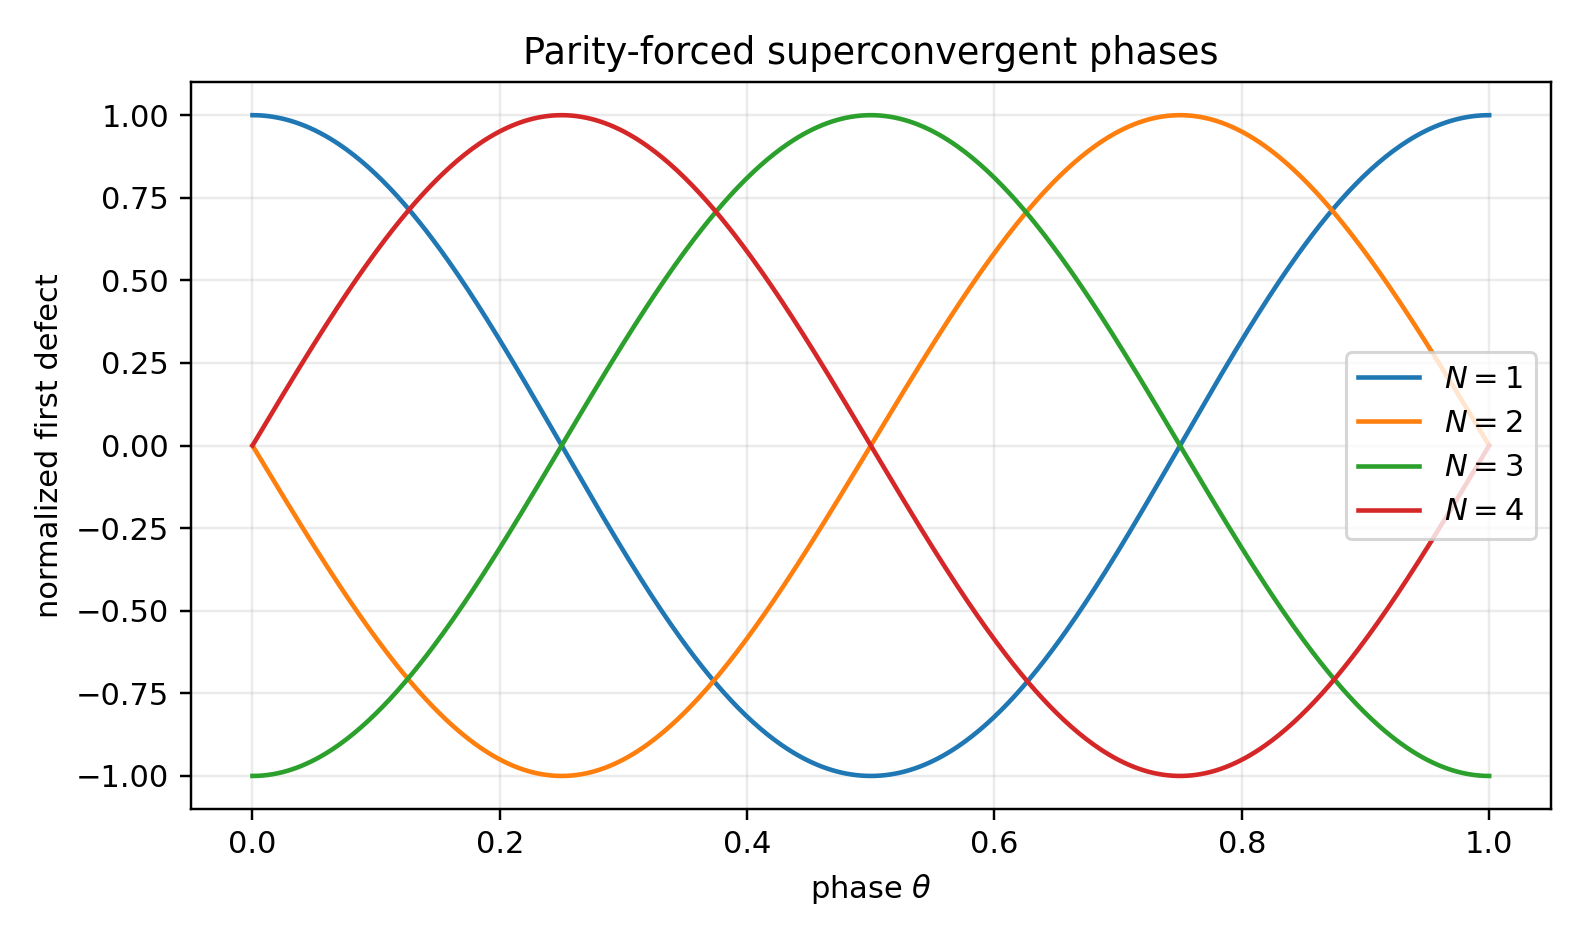
\includegraphics[width=0.88\textwidth]{assets/Fabius_Dyadic_Self_Sampling_Frontier_Package/defect_profiles.png}
\caption{Normalized exact first-defect profiles.  The parity-forced phases are common zeros of every odd harmonic in the corresponding sine or cosine series.}
\label{p3:fig:defect-profiles}
\end{figure}

\subsection{A canonical phase schedule and exact experiments}

Choose
\begin{equation}
 \theta_N=
 \begin{cases}
 0,&N\ \text{even},\\
 1/4,&N\ \text{odd}.
 \end{cases}
 \label{p3:eq:canonical-phase}
\end{equation}
Then $Q_{N,\theta_N}$ is positive, rational, and exact through degree $N+1$.  Its number of positive nodes is $2^{N+1}-1$ at centered levels and $2^{N+1}$ at quarter-shifted levels.

\begin{table}[H]
\centering
\caption{Exact rational checks of the canonical phase schedule.  ``Proved degree'' is the theorem above.  Each next defect is computed as an exact fraction; a decimal display is used here for legibility, while the full fractions are retained in the CSV and exact TeX table in the archive.}
\label{p3:tab:quadrature-exact}
% Generated by experiments.py; exact values are in the CSV
\begin{tabular}{@{}rrrrr@{}}
\toprule
$N$ & phase $\theta_N$ & positive nodes & proved degree & next defect (decimal display)\\
\midrule
0 & $0$ & 1 & 1 & $-0.11111111$\\
1 & $1/4$ & 4 & 2 & $0.011067708$\\
2 & $0$ & 7 & 3 & $0.0002806713$\\
3 & $1/4$ & 16 & 4 & $-2.189698e-6$\\
4 & $0$ & 31 & 5 & $-4.8411566e-9$\\
5 & $1/4$ & 64 & 6 & $3.0609753e-12$\\
6 & $0$ & 127 & 7 & $5.4077218e-16$\\
7 & $1/4$ & 256 & 8 & $-2.6505694e-20$\\
8 & $0$ & 511 & 9 & $-3.5647819e-25$\\
\bottomrule
\end{tabular}

\end{table}

\begin{figure}[H]
\centering
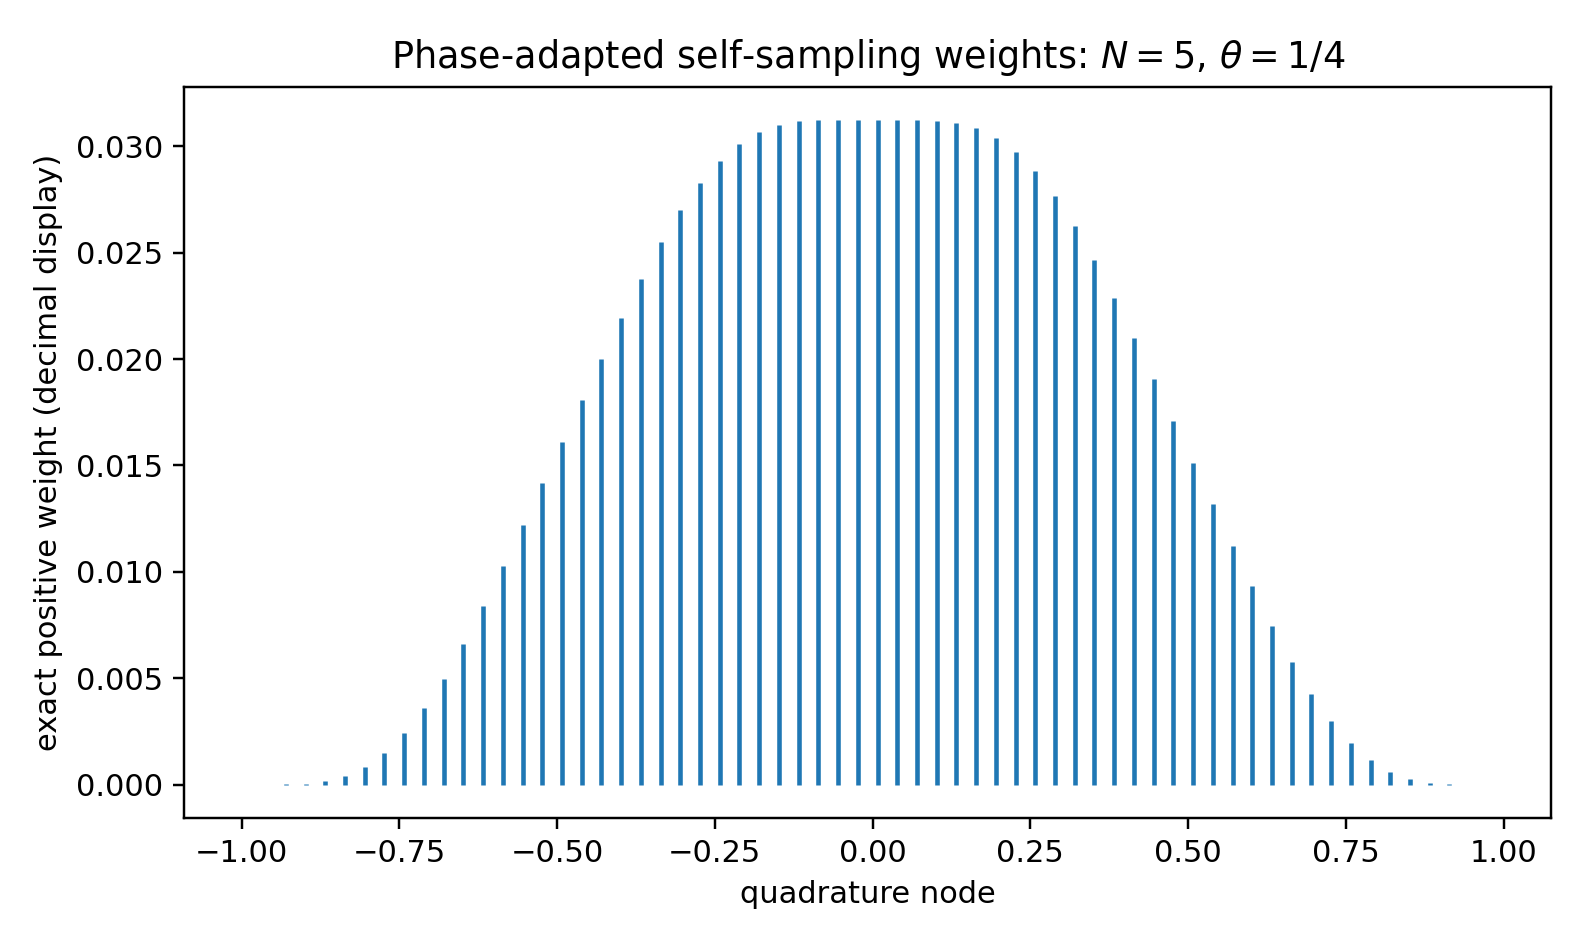
\includegraphics[width=0.88\textwidth]{assets/Fabius_Dyadic_Self_Sampling_Frontier_Package/quadrature_weights.png}
\caption{The positive rational weights at $N=5$, $\theta=1/4$.  The rule integrates every polynomial through degree six exactly.}
\label{p3:fig:quadrature-weights}
\end{figure}

\begin{conjecturebox}[Exact precision conjecture]
For every $N\ge0$, the canonical rule $Q_{N,\theta_N}$ has exact degree $N+1$ and not $N+2$.  Equivalently,
\[
 E_{N,N+2}(\theta_N)\ne0
 \qquad(N\ge0).
\]
The table proves this for $0\le N\le8$ by exact rational arithmetic.  A general proof should use the two-layer decomposition $a=0,1$ in \eqref{p3:eq:valuation-filtration} together with the Bell coefficient $\gamma_1$ in \eqref{p3:eq:gamma1}.
\end{conjecturebox}

\section{Positive alias filters as Richardson extrapolation}
\label{p3:sec:positive-richardson}

\subsection{Coset rules}

For $s\ge0$ and $0\le a<2^s$, define the phase-coset rule
\begin{equation}
 Q_{N;s,a}[f]
 :=2^{-N}\sum_{k\in\Z}
 f\!\left(\frac{2^sk+a}{2^{N+s}}\right)
 u\!\left(\frac{2^sk+a}{2^{N+s}}\right).
 \label{p3:eq:coset-rule}
\end{equation}
This is simply $Q_{N,a/2^s}$, hence is positive and exact through degree $N$.

\begin{theorem}[Positive phase refinement]
\label{p3:thm:positive-phase-refinement}
For every $s\ge0$,
\begin{equation}
 \boxed{\displaystyle
 Q_{N+s,0}[f]
 =2^{-s}\sum_{a=0}^{2^s-1}Q_{N;s,a}[f].}
 \label{p3:eq:positive-phase-refinement}
\end{equation}
Thus averaging all $2^s$ positive phase classes gains exactly $s$ guaranteed degrees of polynomial exactness.
\end{theorem}

\begin{proof}
The integers $2^sk+a$, with $k\in\Z$ and $0\le a<2^s$, partition $\Z$.  Multiplying the outer factor $2^{-N}$ by $2^{-s}$ gives $2^{-(N+s)}$, exactly the fine-grid rule.
\end{proof}

For $s=1$, let
\[
 \nu_N=Q_{N,0},
 \qquad
 \rho_N=Q_{N,1/2}.
\]
Then
\begin{equation}
 \nu_{N+1}=\frac12(\nu_N+\rho_N),
 \qquad
 \boxed{\rho_N=2\nu_{N+1}-\nu_N.}
 \label{p3:eq:midpoint-Richardson}
\end{equation}
The right side is the familiar signed Richardson difference, yet the left side is manifestly a positive quadrature measure.  The cancellation that is hidden in scale space becomes positivity after resolution into even and odd lattice cosets.

\subsection{Uniqueness in alias space}

Suppose coefficients $c_0,\ldots,c_{2^s-1}$ combine the phase classes.  At Fourier alias $\ell$, the multiplier is
\begin{equation}
 C(\ell)=\sum_{a=0}^{2^s-1}c_a\e^{2\pi\iu a\ell/2^s}.
 \label{p3:eq:DFT-filter}
\end{equation}
To gain all $s$ degrees, every residue class $\ell\not\equiv0\pmod{2^s}$ must be annihilated.

\begin{theorem}[Unique full residue-class filter]
\label{p3:thm:unique-phase-filter}
Assume
\begin{equation}
 C(0)=1,
 \qquad
 C(\ell)=0\quad(1\le\ell<2^s).
 \label{p3:eq:DFT-conditions}
\end{equation}
Then
\begin{equation}
 c_0=c_1=\cdots=c_{2^s-1}=2^{-s}.
 \label{p3:eq:unique-uniform-filter}
\end{equation}
Hence the positive average in \eqref{p3:eq:positive-phase-refinement} is the unique filter on all dyadic phases that cancels every nonzero residue class modulo $2^s$.
\end{theorem}

\begin{proof}
The vector $(C(0),\ldots,C(2^s-1))$ is the discrete Fourier transform of $(c_0,\ldots,c_{2^s-1})$.  Inverting the DFT of $(1,0,\ldots,0)$ gives the uniform vector.
\end{proof}

\begin{remark}[Comparison with $q$-Richardson]
The repository's geometric Lagrange/Richardson filters cancel powers of a scale parameter and generally use signed Gaussian-$q$-binomial weights.  The filter above cancels Fourier residue classes and uses equal positive weights.  The two mechanisms act in complementary variables: scale depth versus lattice phase.  Their tensor product is a natural candidate for a stable two-parameter accelerator; see \cref{p3:prob:hybrid-filter}.
\end{remark}

\begin{resultbox}[Third frontier bridge]
Subdividing a self-sampling rule does not merely refine a Riemann sum.  In Fourier space it applies an exact DFT projector to the alias tree.  The usual Richardson difference $2\nu_{N+1}-\nu_N$ is positive because it isolates the odd lattice coset.  This gives a rare instance in which an extrapolation operator has a hidden positive-measure realization.
\end{resultbox}

\section{Inverse-moment Rvachev--Appell polynomials}
\label{p3:sec:appell}

\subsection{The umbral inverse of the moment family}

The frontier volume already uses the forward moment Appell sequence
\begin{equation}
 \Pcal_n(x)=\int_{-1}^{1}(x+y)^n u(y)\dd y,
 \qquad
 \sum_{n\ge0}\Pcal_n(x)\frac{z^n}{n!}=\e^{xz}M(z).
 \label{p3:eq:forward-Appell}
\end{equation}
We now reverse the moment multiplier.

\begin{definition}[Inverse-moment Rvachev--Appell sequence]
\label{p3:def:inverse-Appell}
Define $\Acal_n(x)$ by
\begin{equation}
 \boxed{\displaystyle
 \frac{\e^{xz}}{M(z)}
 =\sum_{n=0}^{\infty}\Acal_n(x)\frac{z^n}{n!}.}
 \label{p3:eq:inverse-Appell-gen}
\end{equation}
\end{definition}

Because $M(0)=1$, this is a well-defined formal power series and an analytic generating function near $z=0$.  Its logarithm is
\begin{equation}
 xz-\sum_{r\ge1}\kappa_{2r}\frac{z^{2r}}{(2r)!}.
 \label{p3:eq:inverse-Appell-log}
\end{equation}

\begin{theorem}[Bell--Bernoulli structure]
\label{p3:thm:Appell-Bell}
The sequence $\Acal_n$ has the following properties.
\begin{enumerate}
\item It is Appell and parity adapted:
\begin{equation}
 \Acal_n'(x)=n\Acal_{n-1}(x),
 \qquad
 \Acal_n(-x)=(-1)^n\Acal_n(x).
 \label{p3:eq:Appell-basic}
\end{equation}
\item It is a complete Bell polynomial in the Bernoulli cumulants:
\begin{equation}
 \boxed{\displaystyle
 \Acal_n(x)=Y_n(x,-\kappa_2,0,-\kappa_4,0,\ldots,-\kappa_n).}
 \label{p3:eq:Appell-Bell}
\end{equation}
\item It satisfies the triangular recurrence
\begin{equation}
 \Acal_{n+1}(x)
 =x\Acal_n(x)
 -\sum_{j=1}^{\floor{(n+1)/2}}
 \binom n{2j-1}\kappa_{2j}\Acal_{n-2j+1}(x).
 \label{p3:eq:Appell-recurrence}
\end{equation}
\item The forward and inverse families are umbral inverses:
\begin{equation}
 M(D)\Acal_n(x)=x^n,
 \qquad
 M(D)^{-1}\Pcal_n(x)=x^n,
 \qquad D=\frac{\dd}{\dd x}.
 \label{p3:eq:umbral-inverse}
\end{equation}
\end{enumerate}
\end{theorem}

\begin{proof}
Differentiate \eqref{p3:eq:inverse-Appell-gen} with respect to $x$ for the Appell law; use the evenness of $M$ for parity.  Equation \eqref{p3:eq:Appell-Bell} is the defining generating identity of complete exponential Bell polynomials applied to \eqref{p3:eq:inverse-Appell-log}.  Differentiating with respect to $z$ gives
\[
 \frac{\partial}{\partial z}\frac{\e^{xz}}{M(z)}
 =\left(x-\frac{M'(z)}{M(z)}\right)\frac{\e^{xz}}{M(z)},
\]
and coefficient comparison gives \eqref{p3:eq:Appell-recurrence}.  Finally, $M(D)$ multiplies an exponential $\e^{xz}$ by $M(z)$, proving \eqref{p3:eq:umbral-inverse} on exponential generating functions.
\end{proof}

The first polynomials are reproduced in \cref{p3:app:Appell-table}.  In compact notation,
\begin{align*}
 \Acal_2(x)&=x^2-\frac19,\\
 \Acal_4(x)&=x^4-\frac23x^2+\frac{31}{675},\\
 \Acal_6(x)&=x^6-\frac53x^4+\frac{31}{45}x^2-\frac{2347}{59535}.
\end{align*}
The constants are the signed complete Bell transforms of the rational cumulants; no transcendental constants remain.

\subsection{Continuous deconvolution}

\begin{theorem}[Exact deconvolution identity]
\label{p3:thm:Appell-deconvolution}
For every $n\ge0$ and $x\in\R$,
\begin{equation}
 \boxed{\displaystyle
 \int_{-1}^{1}\Acal_n(x-y)u(y)\dd y=x^n.}
 \label{p3:eq:Appell-deconvolution}
\end{equation}
Equivalently, the convolution operator by $u$ maps the inverse-moment Appell basis to the monomial basis.
\end{theorem}

\begin{proof}
Multiply generating functions:
\begin{align*}
 \int_{-1}^{1}\frac{\e^{(x-y)z}}{M(z)}u(y)\dd y
 &=\frac{\e^{xz}}{M(z)}M(-z)\\
 &=\e^{xz},
\end{align*}
using the evenness $M(-z)=M(z)$.  Compare coefficients of $z^n/n!$.
\end{proof}

\begin{corollary}[Mean-zero Appell cancellations]
\label{p3:cor:Appell-mean-zero}
For $n\ge1$,
\begin{equation}
 \int_{-1}^{1}\Acal_n(x)u(x)\dd x=0.
 \label{p3:eq:Appell-mean-zero}
\end{equation}
\end{corollary}

\begin{proof}
Set $x=0$ in \eqref{p3:eq:Appell-deconvolution} and use parity.
\end{proof}

\subsection{Finite lattice reproduction}

The self-sampling theorem discretizes the deconvolution identity without loss.

\begin{theorem}[Finite Rvachev--Appell translation formula]
\label{p3:thm:Appell-lattice-reproduction}
Let $N\ge0$, $\theta\in\R$, and $0\le n\le N$.  Then, for every $x\in\R$,
\begin{equation}
 \boxed{\displaystyle
 x^n=2^{-N}\sum_{k\in\Z}
 \Acal_n\!\left(x-\frac{k+\theta}{2^N}\right)
 u\!\left(\frac{k+\theta}{2^N}\right).}
 \label{p3:eq:Appell-lattice-reproduction}
\end{equation}
The sum is finite.  At a superconvergent phase from \cref{p3:cor:forced-superconvergence}, the identity remains valid for $n=N+1$.
\end{theorem}

\begin{proof}
For fixed $x$, the map $y\mapsto\Acal_n(x-y)$ is a polynomial of degree $n$.  Apply \cref{p3:thm:self-sampling} to the integral in \eqref{p3:eq:Appell-deconvolution}.
\end{proof}

More generally, for a polynomial $p$ define its Rvachev deconvolution
\begin{equation}
 \mathscr D_up
 :=M(D)^{-1}p
 =\exp\!\left(-\sum_{r\ge1}\kappa_{2r}
 \frac{D^{2r}}{(2r)!}\right)p.
 \label{p3:eq:polynomial-deconvolution}
\end{equation}
The exponential truncates because $p$ is a polynomial.

\begin{corollary}[Polynomial reproduction by deconvolved translates]
\label{p3:cor:polynomial-deconvolution}
If $\deg p\le N$, then
\begin{equation}
 p(x)=2^{-N}\sum_{k\in\Z}
 (\mathscr D_up)\!\left(x-\frac{k+\theta}{2^N}\right)
 u\!\left(\frac{k+\theta}{2^N}\right).
 \label{p3:eq:general-deconvolution-reproduction}
\end{equation}
\end{corollary}

\begin{resultbox}[Fourth frontier bridge]
The forward moment Appell family packages convolution by the up-law; the reciprocal family $\Acal_n$ packages deconvolution.  The same positive dyadic samples that integrate ordinary polynomials now reproduce ordinary monomials from translates of $\Acal_n$.  This simultaneously connects the Fourier zeros, Bernoulli cumulants, complete Bell polynomials, and finite rational Fabius values.
\end{resultbox}

\subsection{Root geometry: an exact counterexample to real-rootedness}

The first seven polynomials have only real zeros numerically, which makes global real-rootedness a tempting conjecture.  It fails immediately afterward.

\begin{proposition}[First certified nonreal zeros]
\label{p3:prop:A8-roots}
The exact polynomial
\begin{equation}
 \Acal_8(x)
 =x^8-\frac{28}{9}x^6+\frac{434}{135}x^4
 -\frac{9388}{8505}x^2+\frac{1904369}{32531625}
 \label{p3:eq:A8}
\end{equation}
has exactly four real zeros.  Hence its other four zeros are nonreal and form two conjugate pairs.
\end{proposition}

\begin{proof}[Computer-assisted exact proof]
The coefficients lie in $\Q$.  The accompanying script constructs the exact polynomial in $\Q[x]$ from \eqref{p3:eq:Appell-recurrence} and applies a Sturm sequence on $(-\infty,\infty)$.  The exact sign-variation count is four.  No floating-point root classification enters this count.  The certificate and source are included in the archive.
\end{proof}

\begin{figure}[H]
\centering
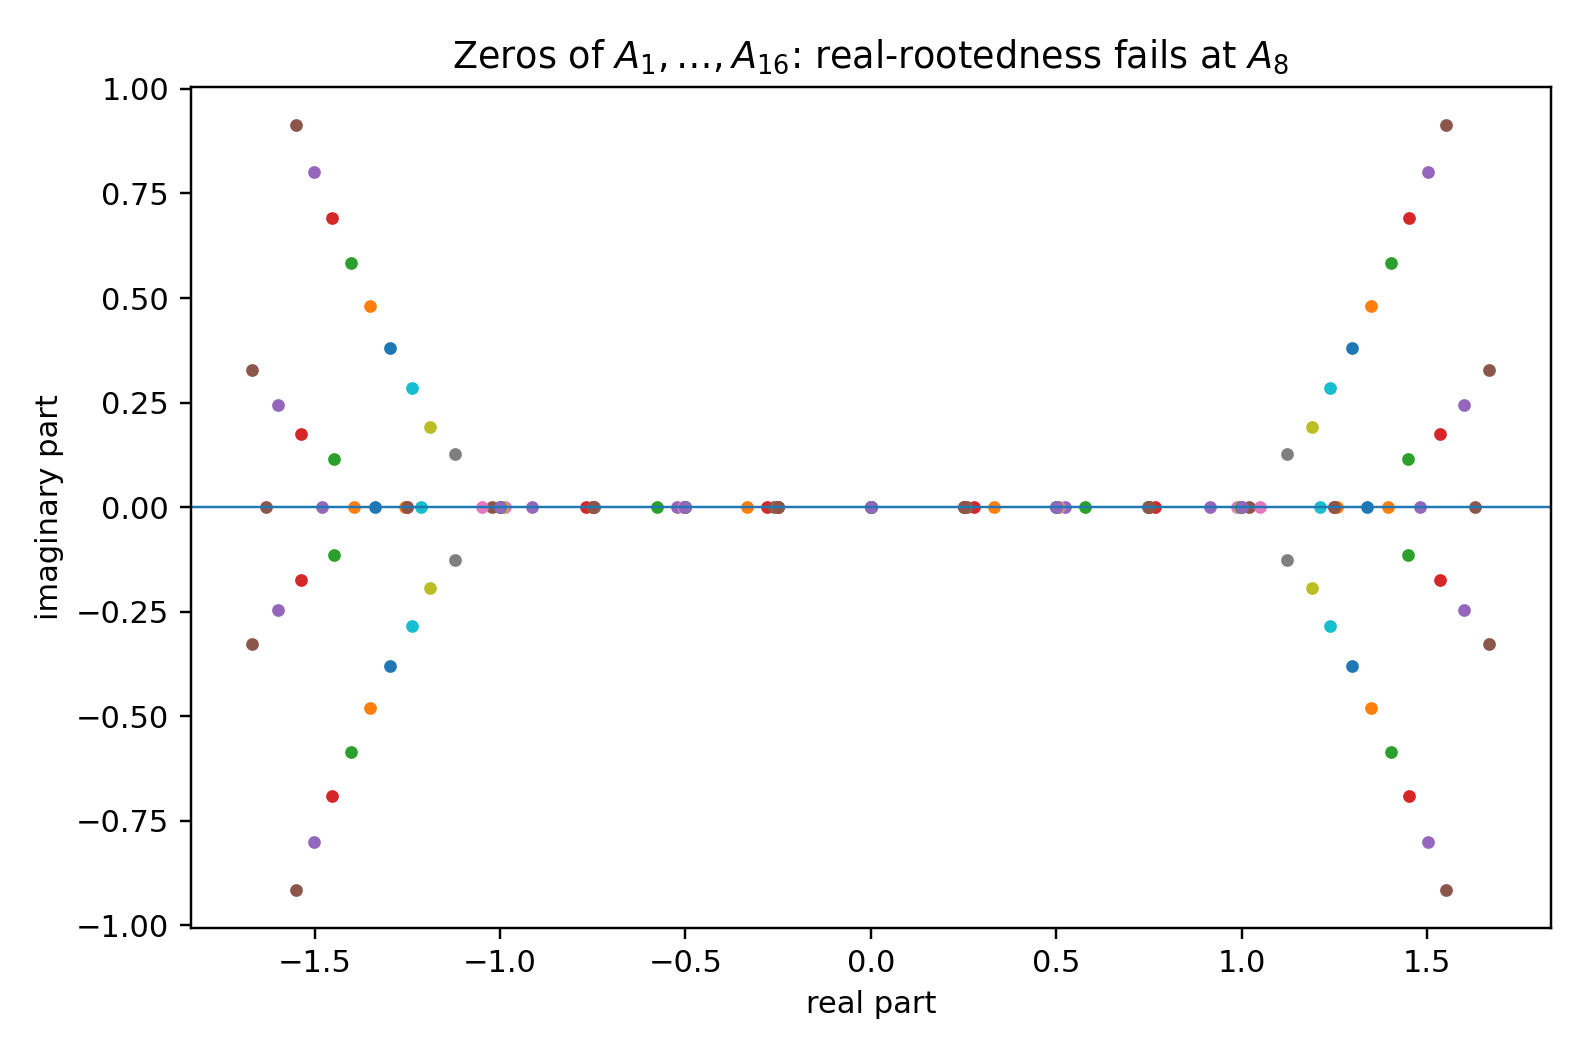
\includegraphics[width=0.86\textwidth]{assets/Fabius_Dyadic_Self_Sampling_Frontier_Package/appell_roots.png}
\caption{Numerical locations of the zeros of $\Acal_1,\ldots,\Acal_{16}$.  The exact Sturm result certifies the first departure from the real axis at degree eight; the later pattern is exploratory.}
\label{p3:fig:Appell-roots}
\end{figure}

The computed nonreal-root counts through degree $30$ are
\begin{center}
\begin{tabular}{@{}lrrrrrr@{}}
\toprule
Degree range & $1$--$7$ & $8$--$12$ & $13$--$17$ & $18$--$22$ & $23$--$28$ & $29$--$30$\\
\midrule
Nonreal roots & $0$ & $4$ & $8$ & $12$ & $16$ & $20$\\
\bottomrule
\end{tabular}
\end{center}
This staircase is not asserted as a theorem; it motivates \cref{p3:conj:Appell-root-staircase}.

\section{Transport through the inverse Fabius function}
\label{p3:sec:inverse-transport}

The centered quantile $q(t)=2F^{-1}(t)-1$ pushes Lebesgue measure on $[0,1]$ to the up-law.  Therefore
\begin{equation}
 \int_0^1g(q(t))\dd t=\int_{-1}^{1}g(x)u(x)\dd x
 \label{p3:eq:quantile-transport}
\end{equation}
for every bounded Borel function $g$.

\begin{theorem}[Rational inverse-Fabius quadrature]
\label{p3:thm:inverse-Fabius-quadrature}
Let $\theta=a/2^s$ and retain the dyadic nodes $x_k=n_k/2^D$ and weights $w_k$ from \cref{p3:cor:rational-rules}.  Define
\begin{equation}
 t_k=F\!\left(\frac{1+x_k}{2}\right)\in\Q.
 \label{p3:eq:inverse-Fabius-nodes}
\end{equation}
Then $q(t_k)=x_k$, and for every polynomial $p$ with $\deg p\le N$,
\begin{equation}
 \boxed{\displaystyle
 \int_0^1p\bigl(2F^{-1}(t)-1\bigr)\dd t
 =\sum_k w_k\,p\bigl(2F^{-1}(t_k)-1\bigr)
 =\sum_k w_kp(x_k).}
 \label{p3:eq:inverse-Fabius-quadrature}
\end{equation}
At a phase-superconvergent level the exactness extends to $\deg p\le N+1$.
\end{theorem}

\begin{proof}
Equation \eqref{p3:eq:centered-CDF} implies $q(t_k)=x_k$.  Apply \eqref{p3:eq:quantile-transport} and then \cref{p3:thm:self-sampling}.  Rationality follows because both $(1+x_k)/2$ and the weight arguments are dyadic.
\end{proof}

\begin{remark}[A nonlinear exactness space]
The rule in \eqref{p3:eq:inverse-Fabius-quadrature} is not claimed to integrate all ordinary polynomials in $t$.  It integrates exactly the non-elementary space
\begin{equation}
 \mathcal V_N
 =\operatorname{span}\{1,q(t),q(t)^2,\ldots,q(t)^N\},
 \qquad q(t)=2F^{-1}(t)-1,
 \label{p3:eq:inverse-exactness-space}
\end{equation}
using rational nodes $t_k$, rational weights $w_k$, and no numerical inversion.  This is an exact finite interface between the inverse Fabius function and dyadic arithmetic.
\end{remark}

\subsection{Endpoint nodes and the Lambert coordinate}

For centered rules, the smallest nonzero endpoint distance is $2^{-N}$ and the corresponding extreme weights are
\begin{equation}
 2^{-N}F(2^{-N}).
 \label{p3:eq:centered-extreme-weight}
\end{equation}
For quarter-shifted rules, the leftmost distance is $2^{-N-2}$, so one extreme weight is
\begin{equation}
 2^{-N}F(2^{-N-2}).
 \label{p3:eq:quarter-extreme-weight}
\end{equation}
The corpus's sharp endpoint theory expresses $F(x)$ through the exact lower-Lambert coordinate
\begin{equation}
 \lambda(x)=-\frac1{\log2}W_{-1}(-x\log2),
 \qquad x=\lambda2^{-\lambda},
 \label{p3:eq:Lambert-coordinate}
\end{equation}
with a nonconstant periodic correction in the dyadic phase of $\lambda$.  Thus the new quadrature rules supply exact rational global moment constraints whose smallest weights lie precisely in the Lambert boundary layer.  Turning these constraints into identities for the endpoint periodic factor is an open program formulated in \cref{p3:prob:Lambert-sum-rules}.

\section{Finite Gaussian-$q$-binomial identities forced by quadrature}
\label{p3:sec:qbinomial}

\subsection{The exact dyadic evaluator}

Let
\begin{equation}
 (q;q)_n=\prod_{j=1}^{n}(1-q^j),
 \qquad
 \qbinom{n}{k}{q}=\frac{(q;q)_n}{(q;q)_k(q;q)_{n-k}}.
 \label{p3:eq:q-notation-report}
\end{equation}
For integers $m,n\ge0$ and $c\in\Q$, define
\begin{equation}
\begin{aligned}
 \mathfrak Q_n(m;c)
 :={}&\frac{1}{2^{n^2}(1/2;1/2)_n}
 \sum_{j=0}^{n}
 \frac{\qbinom{n}{j}{1/2}}
      {2^{j(j-1)}(n+j)!}\\
 &\qquad\times
 \sum_{r=0}^{m2^j-1}\eps_r
 \bigl(r-m2^j+c\bigr)^{n+j}.
 \label{p3:eq:Qfrak-def}
\end{aligned}
\end{equation}
The established arbitrary-numerator theorem states
\begin{equation}
 \mathfrak Q_n(m;c)=F(m/2^n)
 \qquad(0\le m\le2^n),
 \label{p3:eq:Qfrak-F}
\end{equation}
and the right side of \eqref{p3:eq:Qfrak-def} is independent of $c$.  Its Gaussian coefficients arise from Lagrange interpolation on a geometric grid.

\subsection{A $q$-binomial--Thue--Morse--Bell identity}

\begin{theorem}[Finite arithmetic moment identity]
\label{p3:thm:qbinomial-moment-identity}
Let $\theta=a/2^s$, $D=N+s$, $n_k=2^sk+a$, and $b_k=2^D-\abs{n_k}$.  For every $0\le r\le N$ and every $c\in\Q$,
\begin{equation}
 \boxed{\displaystyle
 \mu_r
 =2^{-N-Dr}
 \sum_{\abs{n_k}<2^D}
 n_k^r\,\mathfrak Q_D(b_k;c).}
 \label{p3:eq:qbinomial-moment-identity}
\end{equation}
At the superconvergent phases of \cref{p3:cor:forced-superconvergence}, the identity also holds for $r=N+1$.  Therefore the finite Gaussian-$q$-binomial--Thue--Morse sum on the right equals
\begin{equation}
 Y_r(0,\kappa_2,0,\kappa_4,\ldots,\kappa_r),
 \label{p3:eq:qbinomial-Bell-right}
\end{equation}
where the cumulants are the Bernoulli rationals in \eqref{p3:eq:cumulants}.
\end{theorem}

\begin{proof}
At node $x_k=n_k/2^D$, \eqref{p3:eq:F-up-relation} and \eqref{p3:eq:Qfrak-F} give
\[
 u(x_k)=F(b_k/2^D)=\mathfrak Q_D(b_k;c).
\]
Substitute this into \eqref{p3:eq:self-sampling-main}, then use \eqref{p3:eq:moment-Bell}.
\end{proof}

\begin{remark}[Why this identity is structurally new]
Each ingredient existed separately: the $q$-binomial evaluator, the Bell moment formula, and the zero multiplicities.  The self-sampling theorem forces them into a single positive finite identity.  The common translation $c$ disappears after a double finite summation, giving a family of nontrivial translation-invariance identities among Thue--Morse power sums.
\end{remark}

\begin{corollary}[Finite Appell cancellation in $q$-arithmetic]
\label{p3:cor:q-Appell-cancellation}
For $1\le n\le N$,
\begin{equation}
 \sum_{\abs{n_k}<2^D}
 \Acal_n\!\left(-\frac{n_k}{2^D}\right)
 \mathfrak Q_D(b_k;c)=0.
 \label{p3:eq:q-Appell-cancellation}
\end{equation}
After inserting \eqref{p3:eq:Qfrak-def}, this is a finite identity containing Gaussian $q$-binomial coefficients, Thue--Morse signs, Bernoulli cumulants, and complete Bell polynomials.
\end{corollary}

\begin{proof}
Set $x=0$ in \eqref{p3:eq:Appell-lattice-reproduction} and clear the common factor $2^{-N}$.
\end{proof}

\section{Base-$b$ and multidimensional extensions}
\label{p3:sec:extensions}

\subsection{Integer dilation bases}

Let $b\ge2$ be an integer and define
\begin{equation}
 \Phi_b(\xi)=\prod_{j=0}^{\infty}
 \sincpi\!\left(\frac{\xi}{b^j}\right).
 \label{p3:eq:Phi-b}
\end{equation}
It is the characteristic function of a compactly supported smooth probability density $u_b$, obtained as an infinite convolution of centered uniform laws.  The support radius is $b/(2(b-1))$.

If $m\ne0$ is an integer, then
\begin{equation}
 \ord_{\xi=m}\Phi_b=1+\nu_b(m),
 \label{p3:eq:b-multiplicity}
\end{equation}
where $\nu_b(m)$ is the largest $a$ such that $b^a\mid m$.

\begin{theorem}[Base-$b$ self-sampling]
\label{p3:thm:base-b}
For every $N\ge0$, phase $\theta$, and polynomial $p$ of degree at most $N$,
\begin{equation}
 \int p(x)u_b(x)\dd x
 =b^{-N}\sum_{k\in\Z}
 p\!\left(\frac{k+\theta}{b^N}\right)
 u_b\!\left(\frac{k+\theta}{b^N}\right).
 \label{p3:eq:base-b-self-sampling}
\end{equation}
Moreover, averaging the $b^s$ phases $a/b^s$ gives the level-$N+s$ rule and is the unique full DFT filter annihilating every nonzero residue modulo $b^s$.
\end{theorem}

\begin{proof}
Repeat the Poisson argument.  A nonzero alias $b^N\ell$ has zero order $N+1+\nu_b(\ell)$.  The coset and uniqueness arguments are identical with the $b^s$-point DFT.
\end{proof}

The binary case is distinguished arithmetically because half-integer spectral signs reduce to the classical Thue--Morse sequence and dyadic Fabius values are rational.  For general $b$, the same analytic framework suggests generalized digital sign sequences and $q=b^{-1}$ arithmetic.

\subsection{Tensor-product cubature}

Let
\begin{equation}
 U_d(x_1,\ldots,x_d)=\prod_{j=1}^{d}u(x_j).
 \label{p3:eq:tensor-density}
\end{equation}
Tensoring \cref{p3:thm:self-sampling} gives a positive cubature rule.

\begin{corollary}[Positive tensor cubature]
\label{p3:cor:tensor-cubature}
For a polynomial $p$ whose degree in each coordinate is at most $N$,
\begin{equation}
 \int_{[-1,1]^d}p(\bm x)U_d(\bm x)\dd\bm x
 =2^{-Nd}\sum_{\bm k\in\Z^d}
 p\!\left(\frac{\bm k+\bm\theta}{2^N}\right)
 U_d\!\left(\frac{\bm k+\bm\theta}{2^N}\right).
 \label{p3:eq:tensor-cubature}
\end{equation}
The sum is finite and positive.  Coordinatewise phase superconvergence raises the exactness by one in every selected coordinate.
\end{corollary}

The node count grows exponentially with $d$, so sparse-grid combinations and hyperbolic-cross alias filters are a natural next step; see \cref{p3:prob:sparse-grid}.

\section{Exact and high-precision experiments}
\label{p3:sec:experiments}

The numerical work was designed to test formulas only after they had been derived.  Exact rational arithmetic is used for moments, dyadic Fabius values, quadrature weights, and finite defects.  High-precision floating-point arithmetic is used only for the infinite Fourier products and figures.  Symbolic polynomial arithmetic over $\Q$ is used for the Appell sequence and the Sturm root count.

\subsection{Independent check of the spectral defect}

At the generic dyadic phase $\theta=1/8$, neither parity family is forced to vanish.  For each $0\le N\le7$, the script computes
\[
 Q_{N,1/8}[x^{N+1}]-\mu_{N+1}
\]
exactly from rational Fabius values, and independently evaluates the series in \eqref{p3:eq:first-defect-complex} at 90 decimal digits.

\begin{table}[H]
\centering
\caption{Independent exact-versus-spectral verification at $\theta=1/8$.  The first numerical column is obtained from exact rational arithmetic and displayed decimally; the full fractions are retained in the archive.}
\label{p3:tab:spectral-check}
% Generated by experiments.py at 90 decimal digits
\begin{tabular}{@{}rrrr@{}}
\toprule
$N$ & exact defect (decimal) & spectral series & absolute difference\\
\midrule
0 & $0.121527777778$ & $0.121527777778$ & $2.62e-21$\\
1 & $0.0100171199846$ & $0.0100171199846$ & $2.89e-24$\\
2 & $-0.000295110631872$ & $-0.000295110631872$ & $3.27e-29$\\
3 & $-2.9473755642e-6$ & $-2.9473755642e-6$ & $3.92e-33$\\
4 & $9.14914262587e-9$ & $9.14914262587e-9$ & $5.29e-39$\\
5 & $8.5358933664e-12$ & $8.5358933664e-12$ & $4.92e-44$\\
6 & $-2.32134975825e-15$ & $-2.32134975825e-15$ & $7.03e-51$\\
7 & $-1.80406749858e-19$ & $-1.80406749858e-19$ & $4.21e-57$\\
\bottomrule
\end{tabular}

\end{table}

The residual decreases as more spectral terms become negligible; the displayed discrepancies are truncation errors, not fitted residuals.

\subsection{Exact arithmetic workflow}

The main exact evaluator implements \eqref{p3:eq:finite-F-moment} literally.  A representative excerpt is:

\begin{lstlisting}[style=frontiercode,caption={Exact dyadic Fabius evaluation and shifted moment quadrature.}]
@lru_cache(maxsize=None)
def fabius_dyadic(a: int, n: int) -> Fraction:
    moments = even_moments(n // 2)
    outer = Fraction(0)
    for h in range(a):
        inner = Fraction(0)
        for k in range(n // 2 + 1):
            inner += (Fraction(comb(n, 2*k))
                      * (2*a - 2*h - 1)**(n - 2*k)
                      * moments[k])
        outer += thue_morse_sign(h) * inner
    return outer / (factorial(n) * 2**(n*(n + 1)//2))


def shifted_quadrature_moment(N, degree, a=0, s=0):
    D = N + s
    total = Fraction(0)
    for k in range(-2**N - 2, 2**N + 3):
        numerator = 2**s * k + a
        if abs(numerator) < 2**D:
            x = Fraction(numerator, 2**D)
            total += (Fraction(1, 2**N)
                      * up_dyadic(numerator, D) * x**degree)
    return total
\end{lstlisting}

For every row of \cref{p3:tab:quadrature-exact}, the program first asserts all claimed moment identities exactly and only then writes the next nonzero defect.  The complete, heavily commented script is included in the archive.

\subsection{Reproducibility boundary}

The following distinction is essential:
\begin{itemize}
\item \cref{p3:thm:self-sampling,p3:thm:master-alias,p3:thm:first-defect,p3:thm:Bernoulli-convolution,p3:thm:phase-classification,p3:thm:positive-phase-refinement,p3:thm:Appell-deconvolution,p3:thm:Appell-lattice-reproduction,p3:thm:qbinomial-moment-identity} are proved analytically in the text;
\item the rational tables verify special cases but are not used as proofs of the general identities;
\item \cref{p3:prop:A8-roots} uses an exact computer algebra proof via Sturm's theorem;
\item the root counts beyond degree eight and all plotted root locations are exploratory numerical evidence.
\end{itemize}

\section{Conjectures and frontier research program}
\label{p3:sec:frontier}

\subsection{The next alias layer}

\begin{conjecture}[Exact phase-adapted precision and sign]
\label{p3:conj:next-defect-sign}
Let $\theta_N$ be the canonical phase in \eqref{p3:eq:canonical-phase}.  Then
\begin{equation}
 E_{N,N+2}(\theta_N)\ne0
 \qquad(N\ge0).
 \label{p3:eq:next-defect-nonzero}
\end{equation}
Moreover, for $N\ge1$, the experimental sign law is
\begin{equation}
 \sgn E_{N,N+2}(\theta_N)
 =(-1)^{\floor{(N-1)/2}}.
 \label{p3:eq:next-defect-sign-conj}
\end{equation}
\end{conjecture}

The exact two-layer formula is given in \cref{p3:app:next-defect}.  A proof should combine:
\begin{enumerate}
\item the odd-alias contribution with one Bell correction $\gamma_1$;
\item the twice-odd contribution with its leading zero jet;
\item the parity-specific phase factors;
\item a first-frequency dominance estimate sharp enough to control the logarithmic derivative $\Phi'/\Phi$ at half-integers.
\end{enumerate}
A successful argument would determine the exact degree of every positive phase-adapted rule.

\begin{problem}[All higher phase gains]
\label{p3:prob:higher-phase-gains}
For fixed excess $s\ge2$, classify all phases $\theta$ for which
\[
 E_{N,N+1}(\theta)=\cdots=E_{N,N+s}(\theta)=0.
\]
The valuation filtration makes this a finite hierarchy of trigonometric equations built from alias layers $0,\ldots,s-1$.  Determine whether any single positive phase can gain more than one degree for infinitely many $N$.
\end{problem}

\subsection{Optimal phase and scale filters}

\begin{problem}[Hybrid DFT--Gaussian-$q$ filter]
\label{p3:prob:hybrid-filter}
Combine the positive DFT projector in \eqref{p3:eq:positive-phase-refinement} with the repository's geometric Gaussian-$q$-binomial Richardson filters in the scale variable.  For a prescribed exactness order, minimize:
\begin{enumerate}
\item total variation of the combined coefficients;
\item number of distinct dyadic Fabius evaluations;
\item largest denominator of an exact rational coefficient;
\item sensitivity near the flat endpoints.
\end{enumerate}
A two-stage construction may first remove low $2$-adic alias classes by positive phase averaging and then remove the remaining scale modes by a short signed $q$-Richardson filter.
\end{problem}

\begin{conjecture}[Positive extremality]
\label{p3:conj:positive-extremality}
Among combinations of all $2^s$ dyadic phase classes that gain $s$ degrees uniformly for every level $N$, the uniform average is not only unique under exact residue annihilation, as proved in \cref{p3:thm:unique-phase-filter}, but also minimizes every convex coefficient cost, including $\ell^p$ norms and entropy penalties.
\end{conjecture}

The uniqueness theorem makes this plausible for the full filter.  A subtler variant allows only selected residue classes or allows level-dependent approximate cancellation; then nonuniform positive designs may exist.

\subsection{Denominators and arithmetic geometry}

\begin{problem}[Exact valuations of self-sampling weights]
\label{p3:prob:weight-valuations}
For dyadic $\theta=a/2^s$, determine the exact prime valuations of
\[
 w_{N,\theta,k}=2^{-N}F\!\left(1-\frac{\abs{2^sk+a}}{2^{N+s}}\right)
\]
in lowest terms.  Natural targets are:
\begin{enumerate}
\item exact $2$-adic valuations of the extreme weights;
\item odd-prime divisibility controlled by Mersenne factors $2^{2j}-1$;
\item the least common denominator of the complete rule;
\item cancellation in the rational next defect $E_{N,N+2}(\theta_N)$.
\end{enumerate}
The q-binomial identity \eqref{p3:eq:qbinomial-moment-identity} supplies a second route to the same valuations and may reveal cancellations invisible in the moment formula.
\end{problem}

\begin{conjecture}[Primitive normalized phase rules]
\label{p3:conj:primitive-rules}
After clearing the established common denominator at level $D=N+s$, the integer weight vector of a primitive dyadic phase has greatest common divisor one, except for explicitly classifiable symmetries caused by dyadic refinement.
\end{conjecture}

\subsection{Rvachev--Appell zero geometry}

\begin{conjecture}[Unbounded nonreal root count]
\label{p3:conj:Appell-root-staircase}
The number of nonreal zeros of $\Acal_n$ tends to infinity with $n$.  After scaling $x=n\zeta/(2\pi)$, the zero counting measures converge to a deterministic compact set governed by the nearest poles $z=\pm2\pi\iu$ of $1/M(z)$ and by the dyadic multiplicity hierarchy at $z=\pm2^{j+1}\pi\iu$.
\end{conjecture}

This conjecture is more cautious than extrapolating the short staircase in the data.  General asymptotic theory for Appell polynomials with meromorphic generating functions suggests that the nearest singularities control the zero attractor, but the repeated dyadic pole multiplicities should create nonstandard transitions.

\begin{problem}[A spectral asymptotic for $\Acal_n$]
\label{p3:prob:Appell-spectral-asymptotic}
Use residues of $\e^{xz}/M(z)$ to derive an expansion for $\Acal_n(x)/n!$ that is uniform in the zero-scaling regime.  Determine:
\begin{enumerate}
\item the first curve on which the contributions from $\pm2\pi\iu$ balance;
\item how the next dyadic poles perturb that curve;
\item whether the observed root-count plateaus have an exact spectral explanation;
\item whether a Jensen-polynomial or multiplier-sequence normalization restores real-rootedness.
\end{enumerate}
\end{problem}

\subsection{Lambert endpoint sum rules}

\begin{problem}[Exact quadrature constraints on the periodic endpoint factor]
\label{p3:prob:Lambert-sum-rules}
Insert the repository's all-orders endpoint expansion for $F(x)$, written in the lower-Lambert coordinate \eqref{p3:eq:Lambert-coordinate}, into the exact identities \eqref{p3:eq:centered-moment-F} and \eqref{p3:eq:qbinomial-moment-identity}.  After separating the bulk from a shrinking endpoint boundary layer, derive explicit linear or nonlinear sum rules for the periodic coefficient functions.
\end{problem}

The principal difficulty is uniformity: the number of dyadic samples grows with $N$, while the Lambert expansion is strongest only near the endpoints.  A viable strategy is to choose a cutoff $j\le J(N)$, use the endpoint transseries on that range, and control the remaining samples by smooth quadrature estimates.  Exactness of the full moment identity should force cancellation between the two endpoint layers and the bulk.

\begin{conjecture}[Phase locking of extreme quantile nodes]
\label{p3:conj:quantile-phase-locking}
For the inverse-Fabius quadrature in \eqref{p3:eq:inverse-Fabius-quadrature}, the extreme rational nodes $t_k$ admit a lower-Lambert expansion whose log-periodic phase is locked to the parity schedule \eqref{p3:eq:canonical-phase}.  After the leading endpoint terms are removed, a two-level phase-Richardson combination has an error smaller by a full inverse-Lambert order.
\end{conjecture}

This is deliberately stated as a research conjecture.  The repository already develops inverse-Fabius Lambert--Bell asymptotics; the new question is how those expansions interact with the exact positive moment designs.

\subsection{Digital generalizations and higher dimensions}

\begin{problem}[Base-$b$ spectral signs]
\label{p3:prob:base-b-signs}
For the product \eqref{p3:eq:Phi-b}, determine the sign and phase of $\Phi_b((bk+r)/b)$ on each nonzero residue class $r$.  Identify the resulting automatic sequence and its analogues of Prouhet cancellation, Mahler equations, and $q$-binomial arithmetic.
\end{problem}

\begin{problem}[Sparse-grid Rvachev cubature]
\label{p3:prob:sparse-grid}
Construct Smolyak or hyperbolic-cross combinations of the tensor rules \eqref{p3:eq:tensor-cubature} that preserve as much positivity as possible.  The alias description suggests indexing components by $2$-adic valuation vectors rather than by total scale alone.  Determine optimal node counts for coordinatewise or total-degree exactness.
\end{problem}

\begin{problem}[Nonproduct Rvachev laws]
\label{p3:prob:nonproduct-laws}
Replace the tensor product by compactly supported refinable densities associated with a dilation matrix.  Characterize when Fourier zero multiplicities on the dual lattice make the density's own samples into a positive polynomial cubature rule.
\end{problem}

\section{Lean formalization roadmap}
\label{p3:sec:lean}

The new results divide naturally into four tiers.

\subsection{Tier I: finite arithmetic and Appell algebra}

This tier avoids Fourier analysis and can begin immediately from the existing exact evaluator.
\begin{enumerate}[label=\textbf{I.\arabic*}]
\item Define $\Acal_n$ by the recurrence \eqref{p3:eq:Appell-recurrence} over $\Q[x]$.
\item Prove parity, derivative, and the Bell-polynomial coefficient formula.
\item Verify the explicit polynomials through a chosen degree by reflection.
\item Formalize the exact rational tables in \cref{p3:tab:quadrature-exact} as executable examples, not as substitutes for the analytic theorem.
\item Prove the finite q-binomial substitution identity once self-sampling is available.
\end{enumerate}
Candidate theorem names include
\begin{center}
\begin{minipage}{0.86\textwidth}\small\ttfamily
rvachevAppell\_deriv\\
rvachevAppell\_parity\\
rvachevAppell\_eq\_bell\\
rvachevAppell\_recurrence
\end{minipage}
\end{center}

\subsection{Tier II: Fourier zeros and Poisson summation}

The core analytic theorem requires reusable infrastructure:
\begin{enumerate}[label=\textbf{II.\arabic*}]
\item the infinite sinc product as the Fourier transform of the up density;
\item exact order of the zero at every nonzero integer;
\item shifted Poisson summation for $C_c^\infty$ functions;
\item the derivative-transform identity for $x^ru(x)$;
\item termwise differentiation of the master alias series.
\end{enumerate}
Items II.1 and II.2 are now delivered by \path{FourierProduct.lean},
\path{IntegerZeroLocalFactorization.lean}, and
\path{IntegerZeroAnalyticOrder.lean}.  Items II.3--II.5 remain the analytic
bridge needed for the report-specific self-sampling theorem.
The target statements are
\begin{center}
\begin{minipage}{0.86\textwidth}\small\ttfamily
upSelfSampling\_monomial\\
upSelfSampling\_polynomial\\
upAliasGeneratingFunction\\
upMomentDefect\_valuationSupport
\end{minipage}
\end{center}

\subsection{Tier III: first defect and superconvergence}

Once the analytic layer is in place, formalize:
\begin{enumerate}[label=\textbf{III.\arabic*}]
\item the exact local factorization \eqref{p3:eq:local-factorization};
\item the leading zero jet \eqref{p3:eq:first-zero-jet};
\item the half-integer Thue--Morse sign law;
\item the periodic Bernoulli convolution identity;
\item the elementary lower bound $\Phi(1/2)>4/9$;
\item the trigonometric factor bounds and exact phase classification.
\end{enumerate}
Items III.1 and III.2 are now delivered, and the signed-value identity
underlying III.3 is already in \path{ThueMorseLobeSign.lean}.  Items
III.4--III.6 remain open as formalization tasks.
The Bernoulli convolution may be postponed if periodic distributions are expensive; the sine/cosine series already suffices for superconvergence.

\subsection{Tier IV: probability transport and positive filters}

The final tier is largely algebraic once self-sampling is proved:
\begin{enumerate}[label=\textbf{IV.\arabic*}]
\item positivity and rationality of dyadic weights;
\item phase-coset refinement and DFT uniqueness;
\item Appell deconvolution by formal generating functions;
\item finite Appell translation reproduction;
\item inverse-Fabius transport using the quantile pushforward;
\item base-$b$ and tensor-product generalizations.
\end{enumerate}

\begin{statusbox}[Current compact formalization target]
The integer-zero foundation is now delivered.  The next compact chain is
\[
 \begin{gathered}
 \texttt{shifted Poisson and derivative transform}\\
 \Downarrow\\
 \texttt{self-sampling monomials}\\
 \Downarrow\\
 \texttt{phase superconvergence}.
 \end{gathered}
\]
The exact complex order and leading alias derivative may now be reused
directly rather than reproved inside the quadrature development.
\end{statusbox}

\section{Conclusion}
\label{p3:sec:conclusion}

The dyadic sinc product contains a quadrature rule that is easy to overlook because its nodes and weights are made from the same function.  At mesh $2^{-N}$, every shifted lattice samples the up density into a positive probability measure matching the first $N$ moments exactly.  The proof is one line after the right normalization is chosen: the nonzero Poisson aliases land at integer zeros of multiplicity at least $N+1$.

The first failure is considerably richer.  It is simultaneously
\begin{enumerate}
\item a derivative of the infinite sinc product at its integer zero divisor;
\item a half-integer spectral Dirichlet series with Thue--Morse signs;
\item an exact periodic convolution of a Bernoulli polynomial with a rescaled up-kernel;
\item a parity-sensitive trigonometric function whose only zeros, from level two onward, give the unique phase-superconvergent positive rules.
\end{enumerate}
This four-way identity turns Fourier arithmetic into a practical design principle: centered phases are optimal at even levels, quarter phases at odd levels, and full phase averages implement positive Richardson extrapolation by projecting away alias residue classes.

The reciprocal moment generating function contributes a second new structure.  Its Appell polynomials have rational Bell--Bernoulli coefficients, deconvolve the up-law, and are reproduced exactly by the finite self-sampling measures.  Their root geometry is already nonclassical: exact Sturm arithmetic proves that real-rootedness fails at degree eight.  Substitution of the Gaussian-$q$-binomial dyadic evaluator then converts the analytic quadrature theorem into finite identities involving Lagrange weights, $q$-Pochhammer factors, Thue--Morse power sums, Bernoulli cumulants, and Bell polynomials.

The most promising next steps are now sharply posed: prove the exact next-defect sign, determine denominator valuations, develop the meromorphic zero asymptotics of the inverse Appell family, combine phase DFT filters with scale $q$-Richardson filters, and use the exact moment constraints to interrogate the Lambert-periodic endpoint factor and inverse-Fabius quantiles.  The finite arithmetic and Appell pieces are ready for immediate formalization; the Bernoulli convolution and Poisson layers offer reusable analytic infrastructure for the broader \repoPartl{} project.

\appendix

\section{Complete grouped corpus ledger}
\label{p3:app:corpus}

\subsection{Living documentation treated as authoritative}

\begin{longtable}{@{}p{0.42\textwidth}p{0.52\textwidth}@{}}
\toprule
Path or group & Role in the audit\\
\midrule
\endfirsthead
\toprule
Path or group & Role in the audit\\
\midrule
\endhead
\path{Fabius_Function_and_Rvachev_Up/Fabius_Function_and_Rvachev_Up.tex}
& Primary synthesis: normalization, probability, Fourier theory, exact dyadic values, moment arithmetic, and corrected endpoint asymptotics.\\
\path{FabiusFunction_Mathematical_Glossary/FabiusFunction_Mathematical_Glossary.tex}
& Terminology, notation, and cross-reference check.\\
\path{Non_Elementarity_of_the_Fabius_Function/Non_Elementarity_of_the_Fabius_Function.tex}
& Differential-algebraic and non-elementarity context.\\
\path{fabius_lean_walkthrough/fabius_lean_walkthrough.tex}
& Map between human statements, Lean files, dependencies, and theorem status.\\
\path{non-formalized-research-frontiers/non-formalized-research-frontiers.tex}
& Consolidated gap register and non-formalized frontier synthesis.\\
\path{non-formalized-research-frontiers/drafts/Thue_Morse_Formula_Atlas/Thue_Morse_Formula_Atlas.tex}
& Current formula atlas: digital identities, Prouhet cancellation, Mahler structure, Bell/Bernoulli formulas, and shifted Dirichlet series.\\
\path{non-formalized-research-frontiers/drafts/rvachev_up_fourier_decay/}
& Twelve active manuscripts: initial wave, comparative and second-wave audits, a gentle guide, the asymptotic-product problem statement, successive waves, and final resolution.\\
\path{papers/AIF_76_21-38/}
& Original and corrected TeX transcriptions of Arias de Reyna's compact-support paper.\\
\path{papers/arXiv-1502.06738/}
& Aistleitner--Hofer--Larcher on parametric Thue--Morse sequences and lacunary trigonometric products.\\
\path{papers/arXiv-1702.05442/}
& English translation of Arias de Reyna's 1982 up-function article.\\
\path{papers/arXiv-1702.06487/}
& Arithmetic of dyadic Fabius values.\\
\path{papers/arXiv-2211.13570/}
& Shifted and combined Thue--Morse Dirichlet series.\\
\path{papers/ubiq15/ubiq15-corrected.tex}
& Corrected automatic-sequence background.\\
\bottomrule
\end{longtable}

Within the Fourier-decay family, the inspected subdirectories include
\path{Rvachev_Up_Fourier_Decay-2},
\path{Rvachev_Up_Fourier_Decay-3},
\path{Comparative_Audit},
\path{Gentle_Guide},
\path{Second_Wave_Audit},
\path{asymptotic-decay-rate-of-an-infinite-product-of-sinc-functions},
\path{rvachev_up_fourier_decay-1}, and
\path{rvachev_up_fourier_decay-4} through
\path{rvachev_up_fourier_decay-8}.

\subsection{Frozen archive represented through provenance}

The archive preserves first-introduced historical documents, prunes byte-identical living copies, and retains unique superseded variants.  The following categories were used as a negative-control map.

\begin{longtable}{@{}p{0.20\textwidth}p{0.74\textwidth}@{}}
\toprule
Archive category & Frozen entries\\
\midrule
\endfirsthead
\toprule
Archive category & Frozen entries\\
\midrule
\endhead
Early notes
& \path{Fabius Asymptotic}; \path{K-fold summation over the signed Thue-Morse sequence}.\\
Standalone studies
& \path{Non_Elementarity_of_the_Fabius_Function}; \path{Small_Argument_Asymptotics}; \path{fabius-inverse-dyadic-closed-form}.\\
Primary exposition
& \path{Fabius_Function_and_Rvachev_Up}; \path{Fabius_Function_and_Rvachev_Up-2}; \path{Fabius_Function_and_Rvachev_Up-3}; \path{Fabius_and_Rvachev_Up-2}; \path{Fabius_and_Rvachev_up}; \path{Fabius_function_and_up_function}.\\
Primary supplements
& \path{Fabius_Function_Missing_Parts}; \path{Fabius_Function_Missing_Parts-2}.\\
$q$-calculus
& \path{Fabius_q_Special_Functions}; \path{fabius-q-special-functions}.\\
Lean walkthrough
& Two frozen walkthrough variants recorded under the archive's \path{lean-walkthrough} category.\\
Glossary
& Two frozen glossary variants recorded under the archive's \path{glossary} category.\\
Research frontiers
& \path{Fabius_Dyadic_Asymptotic_Bridge}; \path{Fabius_Dyadic_Formulae_and_Alternative_Representations}; \path{Fabius_Dyadic_Formulae_to_Asymptotics}; \path{Fabius_Dyadic_q_Connections}; \path{Fabius_Thue_Morse_Convergence_Rate}; \path{Fabius_Thue_Morse_Convergence_Rates}; \path{Primary_Exposition_Gap_Register}; \path{Repeated_Integration_and_Rvachev_Up}; \path{Rvachev_Up_from_Repeated_Integration}; \path{non-formalized-research-frontiers}; \path{Thue_Morse_Formula_Atlas-1}; \path{Thue_Morse_Formula_Atlas-2}; \path{Thue_Morse_Formula_Atlas-3}.\\
\bottomrule
\end{longtable}

The archived frontier reports created during the same research program were also treated as negative controls for this report: spectral determinant/zero-zeta results, Pascal--Rvachev hierarchies, rational arithmetic rays, half-integer spectral formulas, logarithmic $q$-Richardson acceleration, positive tail quadrature, and inverse-Fabius Lambert--Bell analysis were not recycled as new claims.

\section{First inverse-moment Appell polynomials}
\label{p3:app:Appell-table}

For compactness the generated table writes $A_n$ in place of $\Acal_n$.
% Generated exactly by experiments.py
\begin{align*}
A_{0}(x)&=1\\
A_{1}(x)&=x\\
A_{2}(x)&=x^{2} - \frac{1}{9}\\
A_{3}(x)&=x^{3} - \frac{x}{3}\\
A_{4}(x)&=x^{4} - \frac{2 x^{2}}{3} + \frac{31}{675}\\
A_{5}(x)&=x^{5} - \frac{10 x^{3}}{9} + \frac{31 x}{135}\\
A_{6}(x)&=x^{6} - \frac{5 x^{4}}{3} + \frac{31 x^{2}}{45} - \frac{2347}{59535}\\
A_{7}(x)&=x^{7} - \frac{7 x^{5}}{3} + \frac{217 x^{3}}{135} - \frac{2347 x}{8505}\\
A_{8}(x)&=x^{8} - \frac{28 x^{6}}{9} + \frac{434 x^{4}}{135} - \frac{9388 x^{2}}{8505} + \frac{1904369}{32531625}\\
A_{9}(x)&=x^{9} - 4 x^{7} + \frac{434 x^{5}}{75} - \frac{9388 x^{3}}{2835} + \frac{1904369 x}{3614625}\\
A_{10}(x)&=x^{10} - 5 x^{8} + \frac{434 x^{6}}{45} - \frac{4694 x^{4}}{567} + \frac{1904369 x^{2}}{722925} - \frac{3309760579}{24405225075}
\end{align*}


\section{Exact two-layer formula for the next defect}
\label{p3:app:next-defect}

Put $R=N+2$.  The valuation filtration \eqref{p3:eq:valuation-filtration} contains only $a=0$ and $a=1$.  For odd $q$, define
\begin{align}
 m_0&=2^Nq,&d_0&=N+1,\\
 m_1&=2^{N+1}q,&d_1&=N+2=R.
\end{align}
Then \cref{p3:cor:Bell-zero-jets} gives
\begin{align}
 \Phi^{(R)}(m_0)
 &=-\frac{R!\Phi(q/2)}{m_0^{N+1}}\gamma_1(m_0),
 \label{p3:eq:next-defect-layer0}\\
 \Phi^{(R)}(m_1)
 &=-\frac{R!\Phi(q/2)}{m_1^R}.
 \label{p3:eq:next-defect-layer1}
\end{align}
Consequently
\begin{equation}
\boxed{
\begin{aligned}
 E_{N,N+2}(\theta)
 =-\frac{R!}{(-2\pi\iu)^R}
 \sum_{\substack{q\in\Z\setminus\{0\}\\q\ \mathrm{odd}}}
 \Phi(q/2)\Bigg[&
 \frac{\gamma_1(2^Nq)}{(2^Nq)^{N+1}}
 \e^{2\pi\iu q\theta}\\
 &+\frac{1}{(2^{N+1}q)^R}
 \e^{4\pi\iu q\theta}\Bigg].
\end{aligned}}
\label{p3:eq:next-defect-exact}
\end{equation}
Here
\begin{equation}
 \gamma_1(2^Nq)
 =-\frac{N+1}{2^Nq}
 +2^{-N-1}\frac{\Phi'(q/2)}{\Phi(q/2)}.
 \label{p3:eq:next-defect-gamma1}
\end{equation}
This formula is the proposed starting point for \cref{p3:conj:next-defect-sign}.  It isolates exactly what is new beyond the first defect: a half-integer logarithmic derivative and one newly activated $2$-adic alias layer.

\section{Reproducibility manifest}
\label{p3:app:repro}

The archive accompanying this report contains:
\begin{longtable}{@{}p{0.38\textwidth}p{0.56\textwidth}@{}}
\toprule
File & Purpose\\
\midrule
\endfirsthead
\toprule
File & Purpose\\
\midrule
\endhead
\path{Fabius_Dyadic_Self_Sampling_Frontier_Report.tex}
& Complete LaTeX source.\\
\path{Fabius_Dyadic_Self_Sampling_Frontier_Report.pdf}
& Rendered report.\\
\path{experiments.py}
& Commented exact rational, high-precision spectral, symbolic Appell, Sturm, table, and figure generator.\\
\path{quadrature_table.csv}, \path{quadrature_table.tex}, \path{quadrature_table_display.tex}
& Exact canonical-phase defects, archival exact table, and compact report table.\\
\path{spectral_check.tex}, \path{spectral_check_display.tex}
& Exact rational versus independent half-integer spectral evaluations, in archival and compact display forms.\\
\path{harmonic_tail_table.tex}
& High-precision first-harmonic tail ratios.\\
\path{appell_polynomials.tex}
& Exact polynomials $\Acal_0,\ldots,\Acal_{10}$.\\
\path{appell_root_counts.csv}
& Exploratory nonreal-root counts through degree $30$.\\
\path{appell_root_certificate.txt}
& Exact polynomial and Sturm root count for $\Acal_8$.\\
\path{defect_profiles.png}
& Normalized first-defect phase profiles.\\
\path{quadrature_weights.png}
& Positive weights of a representative superconvergent rule.\\
\path{appell_roots.png}
& Numerical complex roots through degree $16$.\\
\path{README.txt}
& Commands, dependencies, and file descriptions.\\
\bottomrule
\end{longtable}

The exact checks can be rerun with
\begin{lstlisting}[style=frontiercode]
python experiments.py --no-plots
\end{lstlisting}
and all outputs, including the figures, with
\begin{lstlisting}[style=frontiercode]
python experiments.py
\end{lstlisting}
The script depends only on the Python standard library plus \texttt{mpmath}, \texttt{sympy}, and \texttt{matplotlib}.

\begin{thebibliography}{99}

\bibitem{p3:ProveItPrimary}
V.~Reshetnikov,
\emph{The Fabius Function and Rvachev's Up-Function: Exact arithmetic, probability, Fourier analysis, and corrected sharp asymptotics},
living repository manuscript, 2026.
\url{https://github.com/VladimirReshetnikov/ProveIt/blob/main/Analysis/FabiusFunction/docs/Fabius_Function_and_Rvachev_Up/Fabius_Function_and_Rvachev_Up.tex}

\bibitem{p3:ProveItFrontiers}
V.~Reshetnikov,
\emph{Non-Formalized Research Frontiers for the Fabius Function},
living repository manuscript, 2026.
\url{https://github.com/VladimirReshetnikov/ProveIt/blob/main/Analysis/FabiusFunction/docs/non-formalized-research-frontiers/non-formalized-research-frontiers.tex}

\bibitem{p3:ProveItAtlas}
V.~Reshetnikov,
\emph{A Unified Formula Atlas for the Thue--Morse Sequence},
living repository manuscript, 2026.
\url{https://github.com/VladimirReshetnikov/ProveIt/blob/main/Analysis/FabiusFunction/docs/non-formalized-research-frontiers/drafts/Thue_Morse_Formula_Atlas/Thue_Morse_Formula_Atlas.tex}

\bibitem{p3:AriasUp}
J.~Arias de Reyna,
\emph{An infinitely differentiable function with compact support: definition and properties},
Revista de la Real Academia de Ciencias Exactas, F\'isicas y Naturales de Madrid
\textbf{76} (1982), 21--38; English translation, arXiv:1702.05442.

\bibitem{p3:AriasArithmetic}
J.~Arias de Reyna,
\emph{Arithmetic of the Fabius function},
Integers \textbf{18} (2018), Article A51; arXiv:1702.06487.

\bibitem{p3:Fabius1966}
J.~Fabius,
\emph{A probabilistic example of a nowhere analytic $C^\infty$-function},
Zeitschrift f\"ur Wahrscheinlichkeitstheorie und Verwandte Gebiete
\textbf{5} (1966), 173--174.

\bibitem{p3:Rvachev1990}
V.~A.~Rvach\"ev,
\emph{Compactly-supported solutions of functional-differential equations and their applications},
Uspekhi Matematicheskikh Nauk \textbf{45}, no.~1(271) (1990), 77--103, 222 (in Russian).

\bibitem{p3:StrangFix1973}
G.~Strang and G.~Fix,
\emph{A Fourier analysis of the finite element variational method},
in \emph{Constructive Aspects of Functional Analysis}, Edizioni Cremonese, Rome, 1973, pp.~793--840.

\bibitem{p3:AlloucheShallit}
J.-P.~Allouche and J.~Shallit,
\emph{Automatic Sequences: Theory, Applications, Generalizations},
Cambridge University Press, 2003.

\bibitem{p3:RomanUmbral}
S.~Roman,
\emph{The Umbral Calculus},
Academic Press, 1984.

\bibitem{p3:Comtet}
L.~Comtet,
\emph{Advanced Combinatorics: The Art of Finite and Infinite Expansions},
Reidel, 1974.

\bibitem{p3:CorlessLambertW}
R.~M.~Corless, G.~H.~Gonnet, D.~E.~G.~Hare, D.~J.~Jeffrey, and D.~E.~Knuth,
\emph{On the Lambert $W$ function},
Advances in Computational Mathematics \textbf{5} (1996), 329--359.

\bibitem{p3:FlajoletMellin}
P.~Flajolet, X.~Gourdon, and P.~Dumas,
\emph{Mellin transforms and asymptotics: harmonic sums},
Theoretical Computer Science \textbf{144} (1995), 3--58.

\end{thebibliography}


\end{document}
